%% (Master) Thesis template
% Template version used: v1.4
%
% Largely adapted from Adrian Nievergelt's template for the ADPS
% (lecture notes) project.


%% We use the memoir class because it offers a many easy to use features.
\documentclass[11pt,a4paper,titlepage,oneside]{memoir}

%% Packages
%% ========

%% LaTeX Font encoding -- DO NOT CHANGE
\usepackage[OT1]{fontenc}

%% Babel provides support for languages.  'english' uses British
%% English hyphenation and text snippets like "Figure" and
%% "Theorem". Use the option 'ngerman' if your document is in German.
%% Use 'american' for American English.  Note that if you change this,
%% the next LaTeX run may show spurious errors.  Simply run it again.
%% If they persist, remove the .aux file and try again.
\usepackage[english]{babel}

%% Input encoding 'utf8'. In some cases you might need 'utf8x' for
%% extra symbols. Not all editors, especially on Windows, are UTF-8
%% capable, so you may want to use 'latin1' instead.
\usepackage[utf8]{inputenc}

\usepackage{color,soul}

%% This changes default fonts for both text and math mode to use Herman Zapfs
%% excellent Palatino font.  Do not change this.
\usepackage[sc]{mathpazo}

%% The AMS-LaTeX extensions for mathematical typesetting.  Do not
%% remove.
\usepackage{amsmath,amssymb,amsfonts,mathrsfs}

%% NTheorem is a reimplementation of the AMS Theorem package. This
%% will allow us to typeset theorems like examples, proofs and
%% similar.  Do not remove.
%% NOTE: Must be loaded AFTER amsmath, or the \qed placement will
%% break
\usepackage[amsmath,thmmarks]{ntheorem}

%% LaTeX' own graphics handling
\usepackage{graphicx}

%% We unfortunately need this for the Rules chapter.  Remove it
%% afterwards; or at least NEVER use its underlining features.
% \usepackage{soul}

%% This allows you to add .pdf files. It is used to add the
%% declaration of originality.
\usepackage{pdfpages}

%% URL package
\usepackage{url}

%% Graphics
\usepackage{graphicx}
\usepackage{float}

%% Some more packages that you may want to use.  Have a look at the
%% file, and consult the package docs for each.
%% See the TeXed file for more explanations

%% [OPT] Multi-rowed cells in tabulars
%\usepackage{multirow}

%% [REC] Intelligent cross reference package. This allows for nice
%% combined references that include the reference and a hint to where
%% to look for it.
\usepackage{varioref}

%% [OPT] Easily changeable quotes with \enquote{Text}
%\usepackage[german=swiss]{csquotes}

%% [REC] Format dates and time depending on locale
\usepackage{datetime}

%% [OPT] Provides a \cancel{} command to stroke through mathematics.
%\usepackage{cancel}

%% [NEED] This allows for additional typesetting tools in mathmode.
%% See its excellent documentation.
\usepackage{mathtools}

%% [ADV] Conditional commands
%\usepackage{ifthen}

%% [OPT] Manual large braces or other delimiters.
%\usepackage{bigdelim, bigstrut}

%% [REC] Alternate vector arrows. Use the command \vv{} to get scaled
%% vector arrows.
\usepackage[h]{esvect}

%% [NEED] Some extensions to tabulars and array environments.
\usepackage{array}

%% [OPT] Postscript support via pstricks graphics package. Very
%% diverse applications.
%\usepackage{pstricks,pst-all}

%% [?] This seems to allow us to define some additional counters.
%\usepackage{etex}

%% [ADV] XY-Pic to typeset some matrix-style graphics
%\usepackage[all]{xy}

%% [OPT] This is needed to generate an index at the end of the
%% document.
%\usepackage{makeidx}

%% [OPT] Fancy package for source code listings.  The template text
%% needs it for some LaTeX snippets; remove/adapt the \lstset when you
%% remove the template content.
\usepackage{listings}
\lstset{language=TeX,basicstyle={\normalfont\ttfamily}}

%% [REC] Fancy character protrusion.  Must be loaded after all fonts.
\usepackage{microtype}

%% [REC] Nicer tables.  Read the excellent documentation.
\usepackage{booktabs}


%% Our layout configuration.  DO NOT CHANGE.
%% Memoir layout setup

%% NOTE: You are strongly advised not to change any of them unless you
%% know what you are doing.  These settings strongly interact in the
%% final look of the document.

% Dependencies
\usepackage{ETHlogo}

% Turn extra space before chapter headings off.
\setlength{\beforechapskip}{0pt}

\nonzeroparskip
\parindent=0pt
\defaultlists

% Chapter style redefinition
\makeatletter

\if@twoside
  \pagestyle{Ruled}
  \copypagestyle{chapter}{Ruled}
\else
  \pagestyle{ruled}
  \copypagestyle{chapter}{ruled}
\fi
\makeoddhead{chapter}{}{}{}
\makeevenhead{chapter}{}{}{}
\makeheadrule{chapter}{\textwidth}{0pt}
\copypagestyle{abstract}{empty}

\makechapterstyle{bianchimod}{%
  \chapterstyle{default}
  \renewcommand*{\chapnamefont}{\normalfont\Large\sffamily}
  \renewcommand*{\chapnumfont}{\normalfont\Large\sffamily}
  \renewcommand*{\printchaptername}{%
    \chapnamefont\centering\@chapapp}
  \renewcommand*{\printchapternum}{\chapnumfont {\thechapter}}
  \renewcommand*{\chaptitlefont}{\normalfont\huge\sffamily}
  \renewcommand*{\printchaptertitle}[1]{%
    \hrule\vskip\onelineskip \centering \chaptitlefont\textbf{\vphantom{gyM}##1}\par}
  \renewcommand*{\afterchaptertitle}{\vskip\onelineskip \hrule\vskip
    \afterchapskip}
  \renewcommand*{\printchapternonum}{%
    \vphantom{\chapnumfont {9}}\afterchapternum}}

% Use the newly defined style
\chapterstyle{bianchimod}

\setsecheadstyle{\Large\bfseries\sffamily}
\setsubsecheadstyle{\large\bfseries\sffamily}
\setsubsubsecheadstyle{\bfseries\sffamily}
\setparaheadstyle{\normalsize\bfseries\sffamily}
\setsubparaheadstyle{\normalsize\itshape\sffamily}
\setsubparaindent{0pt}

% Set captions to a more separated style for clearness
\captionnamefont{\sffamily\bfseries\footnotesize}
\captiontitlefont{\sffamily\footnotesize}
\setlength{\intextsep}{16pt}
\setlength{\belowcaptionskip}{1pt}

% Set section and TOC numbering depth to subsection
\setsecnumdepth{subsection}
\settocdepth{subsection}

%% Titlepage adjustments
\pretitle{\vspace{0pt plus 0.7fill}\begin{center}\HUGE\sffamily\bfseries}
\posttitle{\end{center}\par}
\preauthor{\par\begin{center}\let\and\\\Large\sffamily}
\postauthor{\end{center}}
\predate{\par\begin{center}\Large\sffamily}
\postdate{\end{center}}

\def\@advisors{}
\newcommand{\advisors}[1]{\def\@advisors{#1}}
\def\@department{}
\newcommand{\department}[1]{\def\@department{#1}}
\def\@thesistype{}
\newcommand{\thesistype}[1]{\def\@thesistype{#1}}

\renewcommand{\maketitlehooka}{\noindent\ETHlogo[2in]}

\renewcommand{\maketitlehookb}{\vspace{1in}%
  \par\begin{center}\Large\sffamily\@thesistype\end{center}}

\renewcommand{\maketitlehookd}{%
  \vfill\par
  \begin{flushright}
    \sffamily
    \@advisors\par
    \@department, ETH Z\"urich
  \end{flushright}
}

\checkandfixthelayout

\setlength{\droptitle}{-48pt}

\makeatother

% This defines how theorems should look. Best leave as is.
\theoremstyle{plain}
\setlength\theorempostskipamount{0pt}

%%% Local Variables:
%%% mode: latex
%%% TeX-master: "thesis"
%%% End:


%% Theorem environments.  You will have to adapt this for a German
%% thesis.
%% Theorem-like environments

%% This can be changed according to language. You can comment out the ones you
%% don't need.

\numberwithin{equation}{chapter}

%% German theorems
%\newtheorem{satz}{Satz}[chapter]
%\newtheorem{beispiel}[satz]{Beispiel}
%\newtheorem{bemerkung}[satz]{Bemerkung}
%\newtheorem{korrolar}[satz]{Korrolar}
%\newtheorem{definition}[satz]{Definition}
%\newtheorem{lemma}[satz]{Lemma}
%\newtheorem{proposition}[satz]{Proposition}

%% English variants
\newtheorem{theorem}{Theorem}[chapter]
\newtheorem{example}[theorem]{Example}
\newtheorem{remark}[theorem]{Remark}
\newtheorem{corollary}[theorem]{Corollary}
\newtheorem{definition}[theorem]{Definition}
\newtheorem{lemma}[theorem]{Lemma}
\newtheorem{proposition}[theorem]{Proposition}

%% Proof environment with a small square as a "qed" symbol
\theoremstyle{nonumberplain}
\theorembodyfont{\normalfont}
\theoremsymbol{\ensuremath{\square}}
\newtheorem{proof}{Proof}
%\newtheorem{beweis}{Beweis}


%% Helpful macros.
%% Custom commands
%% ===============

%% Special characters for number sets, e.g. real or complex numbers.
\newcommand{\C}{\mathbb{C}}
\newcommand{\K}{\mathbb{K}}
\newcommand{\N}{\mathbb{N}}
\newcommand{\Q}{\mathbb{Q}}
\newcommand{\R}{\mathbb{R}}
\newcommand{\Z}{\mathbb{Z}}
\newcommand{\X}{\mathbb{X}}

%% Fixed/scaling delimiter examples (see mathtools documentation)
\DeclarePairedDelimiter\abs{\lvert}{\rvert}
\DeclarePairedDelimiter\norm{\lVert}{\rVert}

%% Use the alternative epsilon per default and define the old one as \oldepsilon
\let\oldepsilon\epsilon
\renewcommand{\epsilon}{\ensuremath\varepsilon}

%% Also set the alternate phi as default.
\let\oldphi\phi
\renewcommand{\phi}{\ensuremath{\varphi}}


%% Make document internal hyperlinks wherever possible. (TOC, references)
%% This MUST be loaded after varioref, which is loaded in 'extrapackages'
%% above.  We just load it last to be safe.
\usepackage[linkcolor=black,colorlinks=true,citecolor=blue,filecolor=black]{hyperref}


%% Document information
%% ====================

\title{Privacy-Preserving Machine Learning for Cyber Insurance}
\author{T. Giovanna}
\thesistype{Master Thesis}
\advisors{Supervisor: Prof.\ Dr.\ S. Čapkun \\ Advisors: Prof.\ E. Mohammadi, Dr.\ K. Kostiainen}
\department{Department of Computer Science}
\date{February 23, 2021}


%% Make margins the same instead of odd page numbers being indented differently
\setlrmarginsandblock{2.5cm}{2.5cm}{*}
\setulmarginsandblock{2.5cm}{2.5cm}{*}
\checkandfixthelayout

\begin{document}

\frontmatter

%% Title page is autogenerated from document information above.  DO
%% NOT CHANGE.
\begin{titlingpage}
  \calccentering{\unitlength}
  \begin{adjustwidth*}{\unitlength-24pt}{-\unitlength-24pt}
    \maketitle
  \end{adjustwidth*}
\end{titlingpage}

\leavevmode\thispagestyle{empty}\newpage

%% The abstract of your thesis.  Edit the file as needed.
\begin{abstract}
  Cyber risk assessment is an emerging field, in particular for insurance companies, that offer cyber insurance packages to their clients. However, understanding cyber risk is not easy, especially due to the lack of historical data. While machine learning can help, reconciling accuracy, explainability and privacy when data is lacking is challenging. Some machine learning techniques are better than others at addressing these challenges. For instance, ensemble methods such as gradient boosted decision trees (GBDT) are easily explainable, due to their tree structure. This is not the case of other methods such as deep neural networks, which are much more complex to interpret. GBDT models can also provide privacy through differential privacy. However, current state of the arts on differentially private GBDT models suffers from low accuracy when there are limited training data. In this thesis, we propose a new decision tree induction algorithm, \textit{2-nodes}, that enhances accuracy over small datasets while satisfying $\epsilon$-differential privacy. Further, we propose an algorithm based on Bayesian networks to generate synthetic data for cyber risk assessment. Finally, we evaluate our model on various real and synthetic datasets and show that our new induction method is able to improve accuracy on small datasets.
  \end{abstract}


%% TOC with the proper setup, do not change.
\cleartorecto
\tableofcontents
\mainmatter

%% Your real content!
\chapter{Introduction}

\section{Motivation}

In many scenarios where machine learning (ML) is involved, the responsible developing team strives to have an accurate, explainable model. Accurate, because the end goal of an ML model is to help the team in understanding a problem better. Inaccurate outputs would not be helpful. Explainable, because if the team cannot understand the decisions made by the model, in particular the steps involved in these decisions, the problem would remain as complex as it was. Any machine learning model needs a starting point. This starting point usually takes the form of a \textit{training set}. 

The training set contains data about the problem to be learned about, and sometimes data about the solution to be found (\textit{unsupervised} vs. \textit{supervised} learning). In some cases, leakage of the training data creates serious privacy issues, which for some applications is unacceptable. This leads the model to not only require being accurate and explainable, but also to prevent such privacy leaks. One way to prevent these leaks is to train the model in a privacy preserving fashion. Privacy preserving machine learning models can offer guarantees that prevent information about the training data to be extracted. An example application where privacy of the training data is important can be found in assessing \textit{cyber risk}, which we focus on in this thesis.

In recent years, cyber attacks and data breaches have surged, as outlined by recent reports (\cite{verizon_report}, \cite{ibm_report}, \cite{cisco_report}). Companies, large and small, have an increasing need for protection. Such protection not only extends to their technical infrastructure and ability to respond to incidents, but also to potential financial losses that they may face. To cover the latter, insurance companies have come up with cyber insurance products. From the insurer perspective's however, assessing the cyber risk that a particular customer is exposed to is highly challenging. The understanding of cyber risk, i.e. how to describe or model the risk, is not yet as understood as other risks, such as the ones covered by car insurance products.

One major issue that insurers face is trustworthiness when it comes to data provided by their customers. Indeed, customers are often unwilling to disclose their true security practices, fearing that such information could be used to discriminate against them, should they not be complying with or implementing these practices according to the latest industry standards. Currently, these information are collected by insurers through questionnaires that the customers need to fill in. These questionnaires will typically include questions about their security management practices, e.g. details about their software patching process or remote access policy.

\section{Example setting}

One way to address above problems is for insurers to give customers access to an interface allowing them to answer their questionnaires, within a protected space (such as an Intel SGX enclave). This protected space:

\begin{itemize}
	\item can be used to collect sensitive data, while reassuring both the insurers and the customers that no party has direct access to the data.
	\item can be leveraged by customers through remote attestation to verify the correctness of the protected space (i.e. the integrity of any code running within the enclave).
	\item can give customers privacy guarantees with respect to the data they provide.
\end{itemize}

This is represented on the left hand side of Figure ~\ref{fig:big_picture}. In this thesis, we focus on enabling a trustworthy evaluation of the data collected within the protected space. The goal of this evaluation is to train a machine learning model that can be used by insurers to help them evaluate the risk and potential losses associated to the onboarding of a new customer, while providing customers peace of mind about their data. This is represented on the right hand side of Figure ~\ref{fig:big_picture}.

\begin{figure}[h!]
	\center
	\includegraphics[scale=0.75]{images/introduction/big_picture}
	\caption{\label{fig:big_picture} The SGX application on the left hand side, and the privacy preserving machine learning operating within the SGX enclave, zoomed in on the right hand side. SGX application schematic adapted from \cite{sgx_fig}.}
\end{figure}

The insurance company hosts the enclave. The data that the customers send are sent encrypted to the enclave, and never leave it. The data cannot be queried directly, be it by the customers or the insurance company. The SGX enclave can then release the trained model to the insurance company, which can leverage it to learn various kinds of information about the customers. However, due to the privacy preserving properties of the model, the insurance company cannot retrieve information about any single customer.



\section{Chosen approach}

Gradient Boosted Decision Tree (GBDT) models have attracted a lot of attention in recent years and have successfully been used as a winning model in various machine learning competitions\footnote{\href{https://github.com/dmlc/xgboost/tree/master/demo\#machine-learning-challenge-winning-solutions}{https://github.com/dmlc/xgboost/tree/master/demo\#machine-learning-challenge-winning-solutions}}. GBDT models have been shown to be performant, and easily explainable due to their tree structure. In addition, research work (e.g. of Qinbin et al. (2020) \cite{dpgbdt} or Liu et al. (2018) \cite{liu}) has pushed GBDT models towards becoming privacy preserving by leveraging differential privacy. While differential privacy is not the only way to provide privacy (see Chapter ~\ref{chap:related_work}), its strong mathematical foundations and provable properties have made it a de-facto choice in many research work. Although our example setting justifies the attack model that we consider in Chapter ~\ref{chap:security_analysis}, this thesis focuses on the improvement and evaluation of the algorithmic parts: differential privacy applied to gradient boosted decision trees.

\section{Contributions}

While recent work shows encouraging results, developing gradient boosted decision tree models that satisfy $\epsilon$-differential privacy while remaining as accurate as non-private models is still an open challenge, especially when the training data is small, such as in the case of cyber risk evaluation. This thesis aims at addressing the current shortcomings of previous approachs, with the following contributions:

\begin{enumerate} 
	\item We propose a new decision tree induction method, called \textit{2-nodes}, that enhances accuracy over low-populated datasets, while satisfying $\epsilon$-differential privacy. In particular, we propose to make use of extra data in the tree induction process, by finding the optimal splitting point over a node and its sibling's data rather than just the node itself. We use this induction method in an implementation of DP-GBDT that we implement from the literature. This is covered in Chapter ~\ref{chap:2-nodes}.

	\item In Chapter ~\ref{chap:synthetic_data}, and since real data is lacking, we propose a way to generate synthetic datasets that mimic cyber insurance questionnaire answers. To achieve this, we collect figures from cyber security reports written by different vendors in the security and insurance sector, and derive a Bayesian network that we use to compute the dataset's features and targets.

	\item We show in Chapter ~\ref{sec:evaluation} that our model can successfully be used to accurately evaluate cyber risk on 4 different synthetic datasets, as well as improve predictions over low-populated datasets. 
	
	\item We explore privacy attacks on machine learning models in Chapter ~\ref{chap:security_analysis} and apply them to our DP-GBDT model, and show that in some cases it can reduce attack accuracy under strong privacy constraints.
\end{enumerate}


\chapter{Background}

\section{Gradient boosted decision trees (GBDT)}

Dummy text.

\section{Differential privacy}

Dummy text.

\section{Differentially private gradient boosted decision trees (DP-GBDT)}

Dummy text.

\section{Intel SGX}

Dummy text.

\section{Side channels}

Dummy text.
\chapter{Differentially Private Decision Trees}

Differentially private decision tree learning methods aim at preventing information leakage at two levels: when splitting internal nodes, and when querying leaf nodes for prediction results. In \cite{fletcher_survey}, Fletcher et al. (2020) survey differential privacy methods for decision tree learning. They identify the main factors that need to be considered when designing such algorithms: 

\begin{itemize}
	\item \textbf{The privacy budget $\epsilon$}.
	\item \textbf{The number of times the data needs to be queried}. This directly impacts budget consumption. If the data needs to be queried multiple times, then we must apply the sequential composition theorem (Theorem ~\ref{theorem:sequential_composition}). It is clear from the theorem that the more queries there are, the faster the privacy budget will be consumed. The querying strategy of a differentially private model is therefore crucial.
	\item \textbf{The sensitivity $\Delta$ of the queries}. For a fixed privacy objective, tighter sensitivity bounds lead to less added noise, as shown in Theorem ~\ref{theorem:lap} and ~\ref{theorem:exp}: in the Laplace mechanism, reducing the sensitivity $\Delta f$ will reduce the scale of the associated Laplace distribution, hence decreasing the amount of added noise. Equally, in the exponential mechanism, reducing the sensitivity $\Delta u$ will make sure that the chosen attribute's value has a high probability of being amongst the best possible choices.
	\item \textbf{The size of the dataset}. The larger the dataset is, the easier it is for the trees to learn the underlying data structure (since they have access to more data to make better splits), and the least sensitive to noise the trees will be (since a large amount of data will make sure that best splits are chosen with high probability).
\end{itemize}

\section{Related work}

In this section, we explore current and past related work.

\subsection{Privacy budget allocation}\label{sec:budget_allocation}

Jagannathan et al. (2009) \cite{jagannathan} are amongst the first ones to propose a practical differentially private implementation of decision trees for classification problems. They propose a differentially private version of the ID3 algorithm, and show that a naive implementation where counting queries are noised lead to very poor utility under realistic privacy budget constraints. In fact, splitting a privacy budget of $\epsilon=1$ evenly across all queries achieves a classification error rate as high as $81.27\%$ on the nursery dataset\footnote{\href{https://archive.ics.uci.edu/ml/datasets/nursery}{https://archive.ics.uci.edu/ml/datasets/nursery}}. To address this shortcoming, they propose a new approach based on \textit{Random Forest} ensemble methods. Instead of adding noise to each of the queries made during the ID3 algorithm, the decision trees are computed at random and noise is only added to the leaf nodes. This leads to tremendous improvements, with the previously reported error rate dropping to approximately $10.5\%$ for the same dataset and under similar privacy constraints. For comparison, the non-private version of the ID3 algorithm achieves an error rate of $1.81\%$ on the same dataset.

In \cite{mohammed}, Mohammed et al. (2011) split the privacy budget $\epsilon$ into two halves, where each is used for the internal nodes and the leaf nodes respectively ($\epsilon_{node} = \epsilon_{leaf} = \frac{\epsilon}{2}$). Rather than selecting the splitting attribute using noisy counts as in \cite{jagannathan}, Mohammed et al. (2011) propose to use the exponential mechanism (as defined by Theorem ~\ref{theorem:exp}). The main advantage of using the exponential mechanism to select the splitting attribute is that it exponentially favours candidates with a high information gain, hence building more accurate decision trees. In \cite{liu}, Liu et al. (2018) propose to split $\epsilon$ into $s_i$ shares for the selection of internal nodes, based on the $k^{th}$ harmonic number: $s_i = \frac{1}{k} + \frac{1}{k-1} + \dots + 1$. Denoting the budget share for leaf nodes by $s_l = 1$, the total number of shares is $s_t = s_i + s_l$. With $k$ being a fixed, pre-defined number of attributes, Liu et al. (2018) assign $\epsilon_{node} = \frac{\epsilon}{s_t} * \frac{1}{k^2}$ and $\epsilon_{leaf} = \frac{\epsilon}{s_t}.$ Under these constraints, the decision tree satisfies $\epsilon$-differential privacy. We refer the reader to \cite{liu} for a formal analysis of the budget allocation. With the above budget allocation strategies and under Theorem ~\ref{theorem:sequential_composition}, building an ensemble of $T$ decision trees requires a total privacy budget of $\epsilon T$. This means that if the privacy target is $\epsilon$, and because of the data overlap amongst the trees, each tree only receives  a privacy budget of $\epsilon_{t} = \frac{\epsilon}{T}$. As $T$ grows bigger, trees therefore only receive a very small privacy budget, leading to high noise addition and poor accuracy.

Fletcher et al. (2017) \cite{fletcher_smooth} and Li et al. (2020) \cite{dpgbdt} address this shortcoming by proposing an ensemble of trees where each tree operates on a distinct subset of the data. Under these new constraints, each tree within the ensemble can use the full privacy budget: $\epsilon_{t} = \epsilon$. However, this approach doesn't work well on small datasets. Indeed, since every tree operates on its own subset of data, the total number of instances that each tree receives becomes smaller as the number of trees grows bigger. Consider a dataset of $n$ instances $\textbf{X} = X_1,\dots,X_n$ and an ensemble of $T$ trees. Each tree gets roughly $n_{tree} = \ceil{\frac{n}{T}}$ instances. If $T$ is too small, then the learning algorithm suffers from the pitfalls outlined in Section ~\ref{section:decision_trees}. If $T$ is too high, then $n_{tree}$ is small and the decision trees might not have enough instances to learn the underlying structure of the dataset.

In \cite{wen_wang} and \cite{nazanin}, the authors mention an adaptive budget allocation method. Rather than fixing an equal privacy budget used at each depth of the tree, the authors propose to compute this quantity during the tree induction algorithm. In the former case, the budget at each depth $d$ is computed as $\epsilon_{node} = \frac{1}{2^d}\epsilon_{t}$. This exponentially decaying budgeting is motivated by the intuition that early splits in the tree are more important than subsequent splits, hence why they get a higher portion of the privacy budget. However, such an allocation method might not be ideal when the tree gets very deep, as lower levels in the tree will receive a really small budget, which in turn creates too much noise and penalizes the quality of the tree. In the latter, the author proposes a new induction algorithm, \textit{ADiffP-$\phi$}, that computes each split's privacy budget dynamically and uses it as a termination criteria when the budget gets too small. Thus, the total number of nodes in the tree is not controlled by the maximum depth (or any other usual termination criteria), but by the total privacy budget available to the tree.

\subsection{Query sensitivity}\label{sec:query_sensitivity}

Fletcher and Islam (2015) \cite{fletcher_local} explore reducing the sensitivity of the splitting functions, hopping to reduce the amount of noise added in the tree-building process. Rather than computing the global sensitivity of a function, they propose to compute the local sensitivity of the Gini index in the node being split as $\Delta = 1 - (\frac{n_i}{n_i + 1})^2 - (\frac{1}{n_i + 1})^2$ where $n_i$ is the support of node $i$ (the support is equal to the number of instances in the node). This sensitivity reduction directly improves the Laplace and exponential mechanisms, as a tighter sensitivity bound allows for lower added noise. However, in its current form, this sensitivity derivation might be too noisy in some cases and incorrectly providing differential privacy. The same authors later proposed additional work (\cite{fletcher_signal}, \cite{fletcher_smooth}) based on Nissim et al. (2007) \cite{nissim}'s smooth sensitivity definition to enhance their model.

In \cite{dpgbdt}, Quinbin et al. (2020) propose a new way to bound the sensitivity of both the leaf nodes and the splitting function. Using new procedures (\textit{Geometric Leaf Clipping} and \textit{Gradient-based Data Filtering)}, they proved that the sensitivity of the leaf nodes could be bound by $\Delta V \leq \min(\frac{g_l^*}{1 + \lambda},2g_l^*(1-\eta)^{t-1})$ and that the sensitivity of the splitting function could be bound by $\Delta G \leq 3g_l^{*2}$, where $g_l^*$ is the maximum possible 1-norm gradient, $\lambda$ is a regularisation parameter, $\eta$ is the learning rate and $t$ is the index of the tree being constructed. These new bounds offer better accuracy in the differentially private settings.

Wang et al. (2020) \cite{wen_wang} introduce the first provably accurate privacy preserving, top-down decision tree learning algorithm in the distributed setting. More information about top-down algorithms can be found in \cite{kearns}. They propose a new splitting function, \texttt{PrivateSplit}, that approximates the optimal split chosen by the top-down algorithm, while providing differential privacy and proving boosting-based utility guarantees. In fact, they show that their algorithm only needs $(1/\epsilon)^{O(\log(1/\epsilon)/\gamma^2)}$ splits to achieve a training error $\leq \epsilon$ with probability $\geq 1-\delta$ (provided that the dataset has a certain size). On the adult dataset\footnote{\href{https://archive.ics.uci.edu/ml/datasets/adult}{https://archive.ics.uci.edu/ml/datasets/adult}}, their algorithm achieves roughly $79\%$ accuracy, which is a little over Quibin et al. (2020) \cite{dpgbdt}'s accuracy (roughly $74\%$) over the same dataset and under the same privacy budget constraints $\epsilon = 1$.

\subsection{Termination criteria and post-processing}

When building a decision tree, one must choose some criteria as to when to stop growing the tree. The simplest criterion is to stop growing the tree once it reaches a certain depth $d$. Other termination criteria include defining a maximum number of leaf nodes that a tree can have, or defining a minimum number of samples that a node must have before being split (i.e. a minimum node support). However, there is no optimal value for any of these criteria that works for every dataset. Rather, it is left to the user to find appropriate values that work best for their use case. In some cases, these parameters may be estimated based on the dataset. In \cite{fan}, the authors limit the tree depth to $d = \frac{k}{2}$ where $k$ is the number of features in the dataset. In \cite{jagannathan}, the tree depth is set to $d = \min(k/2, \log_b(n) - 1)$ where $n$ is the size of the dataset, and $b$ is the branching factor.

Once the tree has reached its termination criteria, one can apply post-processing methods, such as \textit{pruning}, to the tree. Pruning consists in removing untrustworthy leaf nodes from the tree. A leaf node can be considered untrustworthy if its support or purity (homogeneity of the class labels in the node) is too low. In the differentially private settings, pruning cannot be applied as it is in traditional decision trees, as the modifications to the tree induction algorithm induced by differential privacy need to be accounted for. Friedman and Schuster (2010) \cite{friedman_schuster} adapt classical pruning mechanisms by normalising the support of each node in the tree, so that that sum of all counts in all nodes matches the size of the dataset (which is not initially the case due to the noise introduced by differential privacy). In random forests, Fletcher and Islam (2015) \cite{fletcher_signal} observe that in some cases, an additional split worsens the decision tree rather than help it, since the split is chosen at random. They therefore propose to prune leaf nodes where the added noise is greater than the class count signal.

\subsection{Depth-first and best-leaf first decision tree induction}\label{sec:growth}

There are several ways to grow a decision tree during its induction process. While most algorithms grow trees by level, i.e. depth-wise, some implementations (like XGBoost \cite{xgboost}) grow decision trees with a best-leaf first approach. This approach was first described by Haijian S. (2007) \cite{shi} in his doctoral thesis. Figure ~\ref{fig:tree_dfs} and ~\ref{fig:tree_bfs} show the differences between a depth-first and a best-leaf first tree induction algorithm (the figures are adapted from XGboost documentation\footnote{\href{https://github.com/Microsoft/LightGBM/blob/master/docs/Features.rst}{https://github.com/Microsoft/LightGBM/blob/master/docs/Features.rst}}).

\begin{figure}[h!]
	\center
	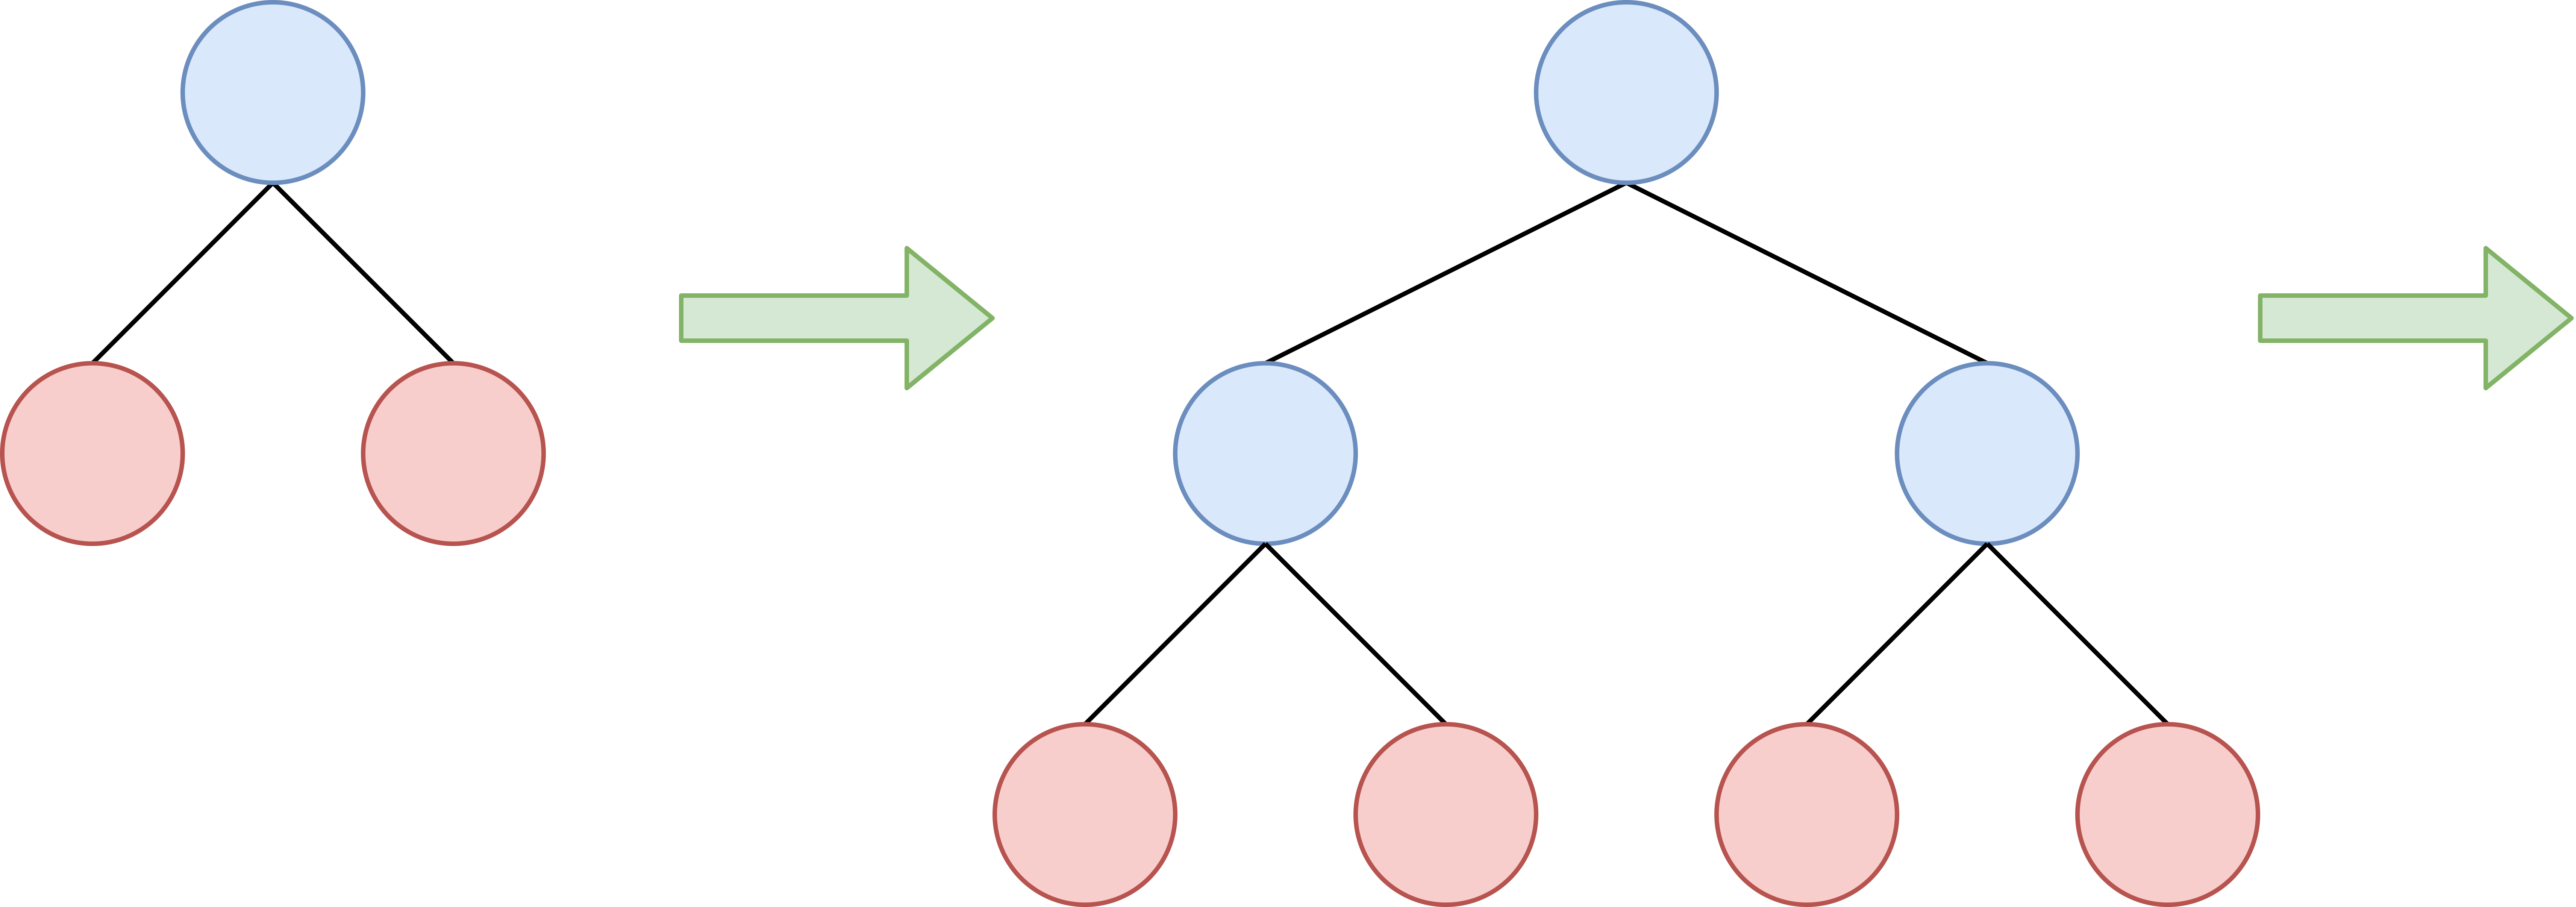
\includegraphics[scale=0.7]{images/dpgbdt/dfs}
	\caption{\label{fig:tree_dfs} A depth-first decision tree induction algorithm.}
\end{figure}

\begin{figure}[h!]
	\center
	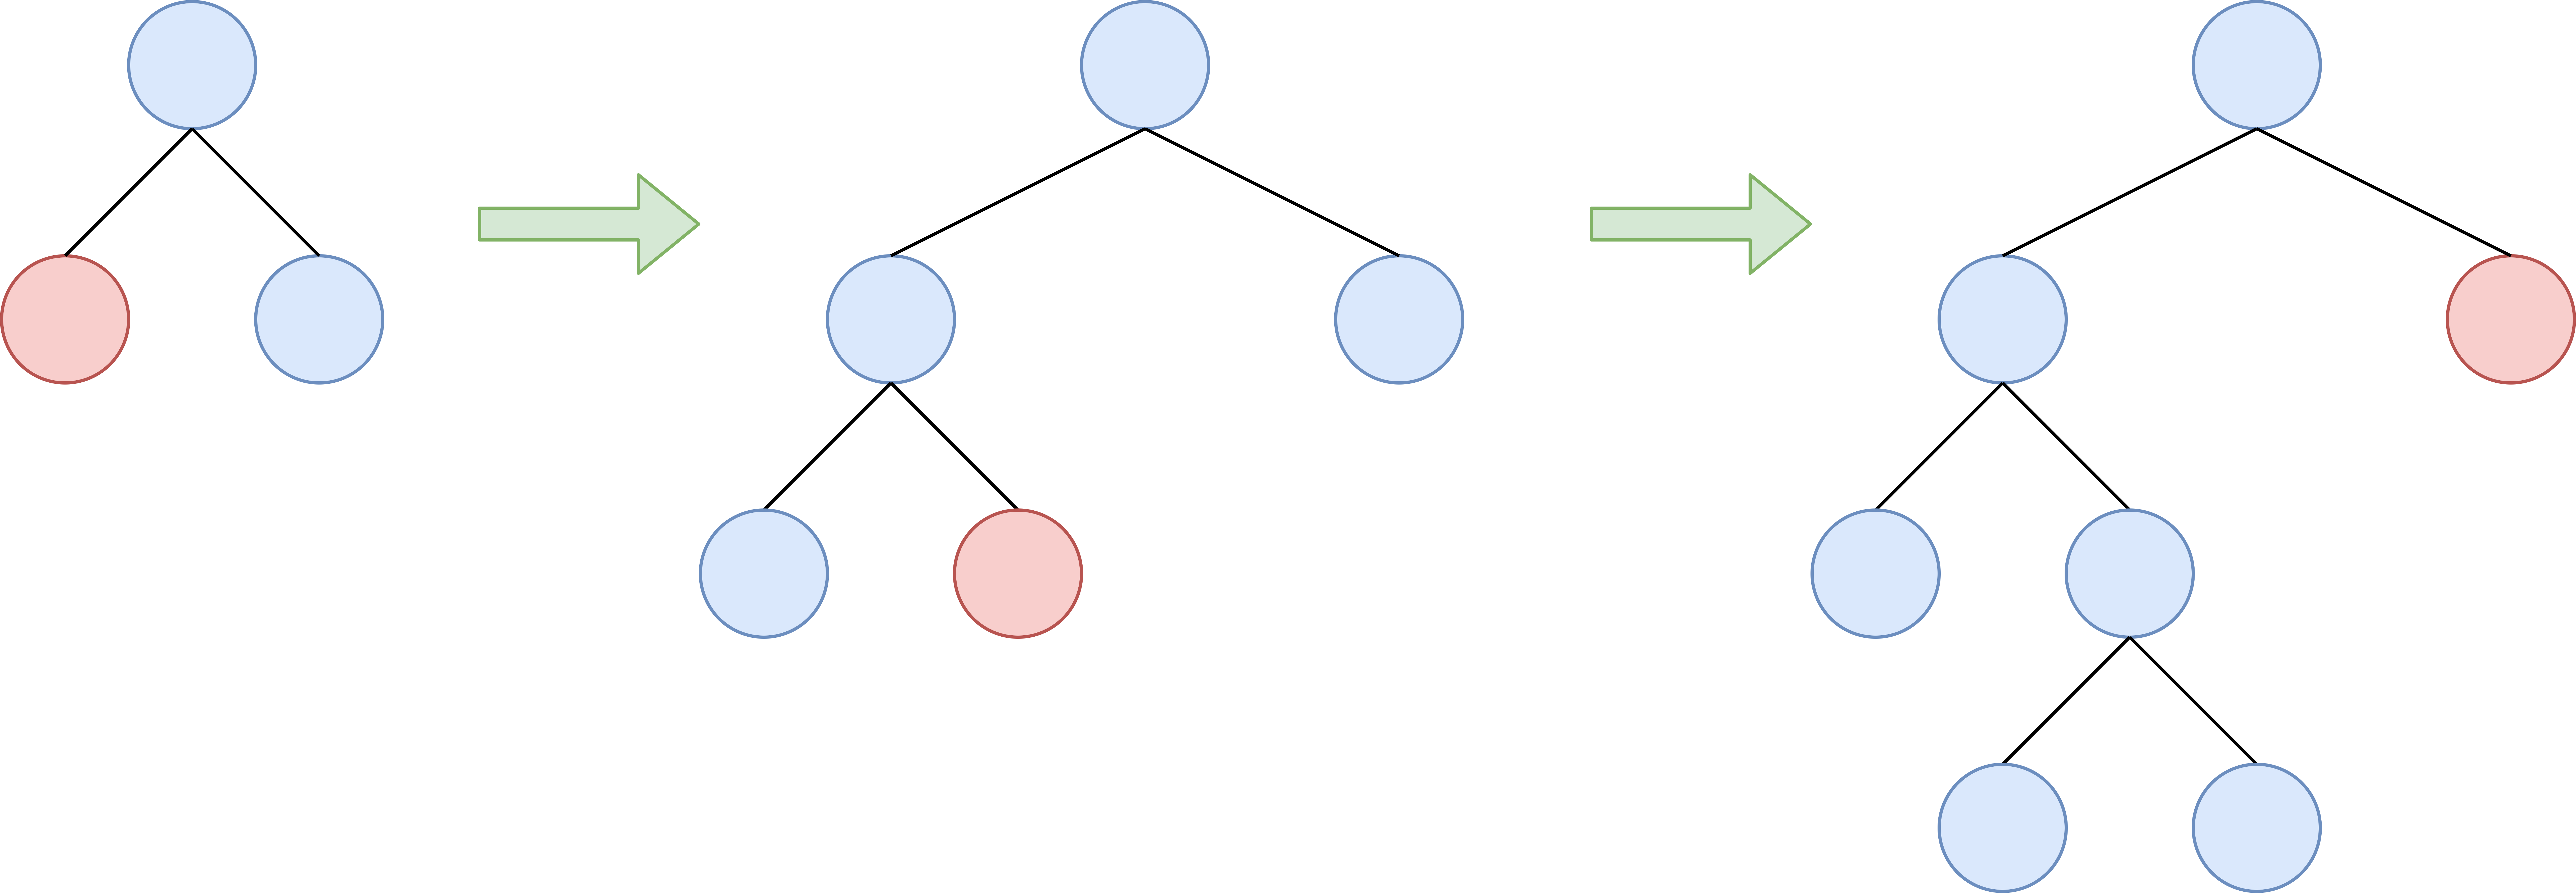
\includegraphics[scale=0.7]{images/dpgbdt/bfs}
	\caption{\label{fig:tree_bfs} A best-leaf first decision tree induction algorithm.}
\end{figure}

Depending on the dataset, a best-leaf first induction might achieve a lower loss. However, when the number of data is small, a best-leaf first approach may over-fit the dataset. 

In the next section, we choose to explore in more details the work of Quibin et al. (2020) \cite{dpgbdt}. This choice is motivated by the tight sensitivity bounds that the authors were able to derive, along with the good prediction accuracy that their model showed.


\section{Differentially private gradient boosted decision trees (DP-GBDT)}

To make decision trees differentially private with the definitions provided in Section ~\ref{sec:dp}, the literature (\cite{inprivate}, \cite{mohammed}, \cite{dpgbdt}) proposes two changes to Algorithm ~\ref{algo:gbdt}:
\begin{itemize}
	\item For each node, the attribute and the attribute's value on which the node is split must be chosen through the exponential mechanism. The information gain $G$ is used as the utility function, and the exponential mechanism guarantees that the attributes and attributes' value with higher gain have a higher probability of being chosen.
	\item For each leaf node, the leaf value must be noised through the Laplace mechanism.
\end{itemize}

Qinbin et al. (2020) \cite{dpgbdt} suggests that each tree $t$'s privacy budget $\epsilon_t$ gets split into two parts: $\epsilon_{leaf} = \frac{\epsilon_t}{2}$ for the leaf nodes and $\epsilon_{node} = \frac{\epsilon_t}{2d_{max}}$ for the internal nodes, where $d_{max}$ is the maximum depth for the tree $t$. Since the nodes in one depth have disjoint inputs, Theorem ~\ref{theorem:parallel_composition} can be applied and the privacy budget in one depth needs to be counted only once. Thus, the total privacy budget consumption is no more than $\epsilon_{node} * d_{max} + \epsilon_{leaf} = \epsilon_t$. Once a tree is trained, the gradients of all instances are updated. This allows the next tree to converge towards a minimum for the objective function defined in Equation ~\ref{eq:gbdt_obj}. The authors propose Algorithm ~\ref{algo:dp_gbdt}.

\begin{algorithm}
	\DontPrintSemicolon
	\SetKwComment{Comment}{$\triangleright$\ }{}
	\SetCommentSty{itshape}
	\caption{Differentially private GBDTs training process \cite{dpgbdt}}\label{algo:dp_gbdt}
	\KwIn{$\textbf{X} = X_1,\dots,X_n$: instances, $\textbf{y} = y_1, \dots, y_n$: labels}
	\KwIn{$\lambda$: regularisation parameter, $d_{max}$: maximum depth, $\eta$: learning rate}
	\KwIn{$T$: total number of trees, $l$: loss function, $\epsilon$: privacy budget}
	\KwOut{An ensemble of trained differentially private decision trees.}
	$\epsilon_t$ = $\epsilon$ \ \Comment*[r]{\textcolor{blue}{Each tree is trained on a disjoint subset of the dataset, so we can apply Theorem ~\ref{theorem:parallel_composition}}}
	\For{$t=1$ \textbf{to} $T$}{
		Update gradients of all training instances on loss $l$ \;
		$\epsilon_{leaf} = \frac{\epsilon_t}{2}, \; \epsilon_{node} = \frac{\epsilon_t}{2d_{max}} $ \;
		\For{d = 1 \textbf{to} $d_{max}$}{
			\For{\textit{each node in current depth}}{
				\For{\textit{each split value i}}{
					$G_i \gets \frac{(\sum_{i \in I_L}g_i)^2}{|I_L| + \lambda} + \frac{(\sum_{i \in I_R}g_i)^2}{|I_R| + \lambda}$ \Comment*[r]{\textcolor{blue}{Equation ~\ref{eq:gbdt_gain_simplified}}}
					$P_i \gets \exp(\frac{\epsilon_{node} \cdot G_i}{2 \Delta G})$ \Comment*[r]{\textcolor{blue}{Theorem ~\ref{theorem:exp}}}
				}
				Split node on split value $i$, where $i$ is chosen with probability $P_i / \sum_j P_j $
			}
		}
		\For{\textit{each leaf node i}}{
			$V_i \gets \eta \left(-\frac{\sum_{i \in I}g_i}{|I| + \lambda} + Lap(0, \Delta V/\epsilon_{leaf}) \right)$ \Comment*[r]{\textcolor{blue}{Equation ~\ref{eq:gbdt_leaf_value} and Theorem ~\ref{theorem:lap}}}
		}
	}
\end{algorithm}

The authors use the parallel composition theorem (Theorem ~\ref{theorem:parallel_composition}) to lower the privacy budget consumption by training each decision tree on a disjoint set of data. However, when the training dataset is small and the number of trees is large, each tree only gets very few samples to learn from. This low number of samples available to the trees results in bad splits, which damages the quality of the trees and their predictions. To address this limitation, we propose in the next chapter a new induction algorithm, \textit{2-nodes}.

\chapter{2-nodes Algorithm}\label{chap:2-nodes}

Our model was implemented in Python 3, and is available on GitHub\footnote{\href{https://github.com/giovannt0/dpgbdt}{https://github.com/giovannt0/dpgbdt}}. Our base implementation follows \cite{dpgbdt}, with their own implementation (based on XGBoost \cite{xgboost}) available on GitHub as well\footnote{\href{https://github.com/QinbinLi/DPBoost}{https://github.com/QinbinLi/DPBoost}}. We implemented the following features:

\begin{itemize}
	\item Gradient based data filtering and geometric leaf clipping (from \cite{dpgbdt}, described in Section ~\ref{sec:query_sensitivity}). This can be enabled or disabled.
	\item Depth-first, best-leaf first and 2-nodes tree induction, outlined in Section ~\ref{sec:growth} and in this chapter.
	\item Decaying privacy budget (from \cite{wen_wang}, described in Section ~\ref{sec:budget_allocation}). This can be enabled or disabled.
\end{itemize}

\section{Design}

The 2-nodes induction method (Figure ~\ref{fig:tree_2-nodes}) is a modified version of the classical depth-first tree growth algorithm outlined in Figure ~\ref{fig:tree_dfs}. At each depth $d$ of the tree, for a given node $n_{d_i}$, $0 \leq d < d_{max}$ and $0 \leq i < 2^d$, we consider the data-points of the sibling node $n_{d_j}$ ($j$ being the index of the node that shares the same parent node as $n_{d_i}$) while computing the optimal splitting point.
The reason we opted for this design is that the exponential mechanism (used to select the splitting point) performs better the more instances there are within a node, as the gain and associated probabilities will be higher (see Equation ~\ref{eq:gbdt_gain_simplified}). By combining instances in the nodes and their siblings, we can make sure that the chosen splits will fit the data better.

\begin{figure}[h!]
	\center
	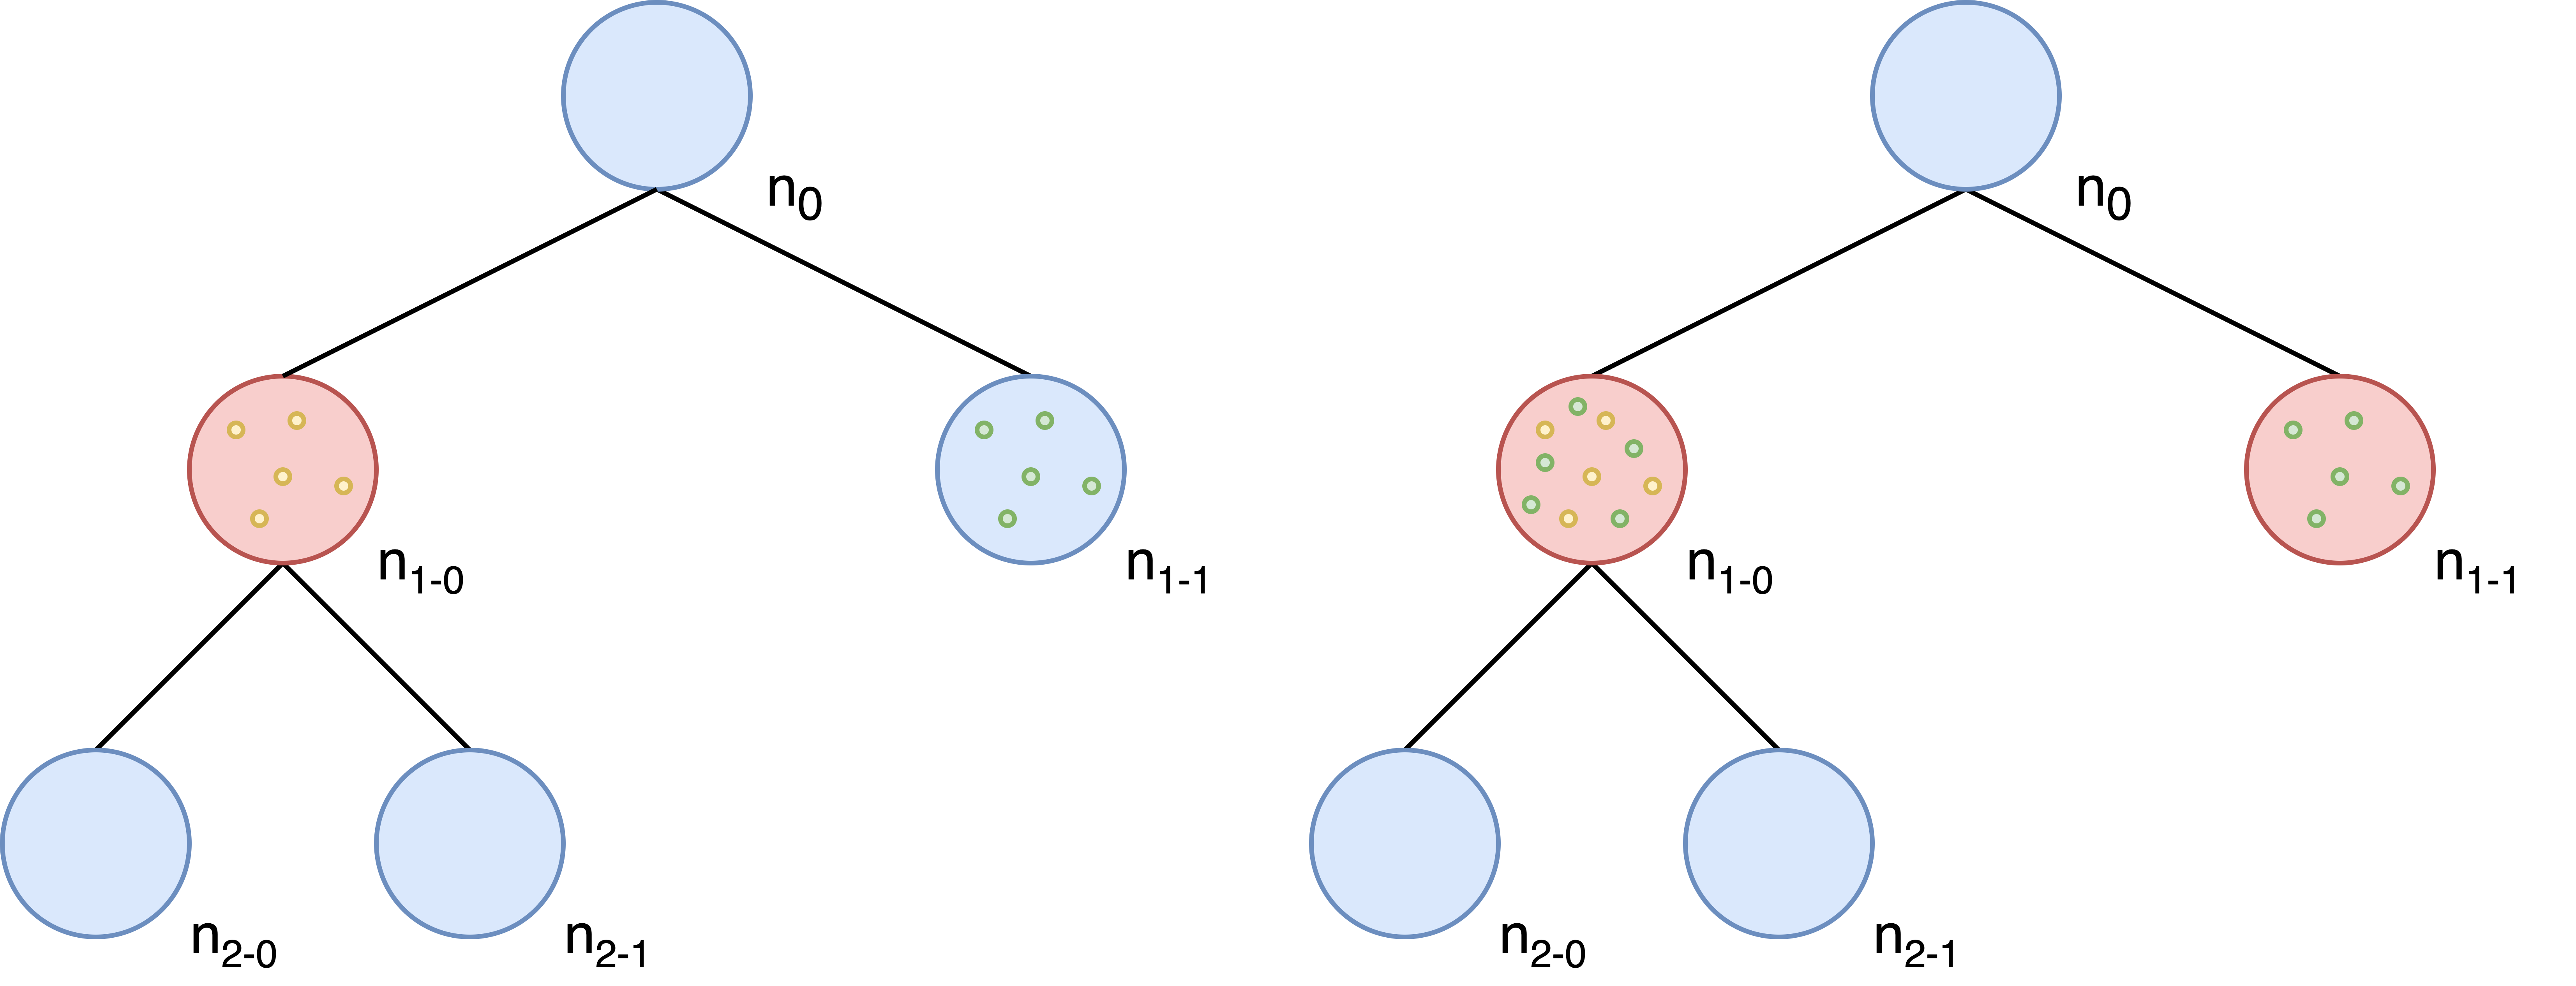
\includegraphics[scale=0.66]{images/dpgbdt/2-nodes.png}
	\caption{\label{fig:tree_2-nodes} Data-points (red nodes) being considered while splitting a node for the depth-first (left) vs. 2-nodes (right) algorithms. In the depth-first case, node $n_{1_0}$'s best split is computed over the instances of the node itself. In the 2-nodes case, node $n_{1_0}$'s best split is computed on the instances of the node itself, and the instances of its sibling node $n_{1_1}$.}
\end{figure}

\section{Properties}

In a differentially private scenario, the data-points in each node (except the root node) at every level will be queried twice (once when splitting the node, and once when splitting its sibling node). We can therefore adapt Algorithm ~\ref{algo:dp_gbdt} into Algorithm ~\ref{algo:2_nodes_dpgbdt}.

\begin{algorithm}
	\DontPrintSemicolon
	\SetKwComment{Comment}{$\triangleright$\ }{}
	\SetCommentSty{itshape}
	\caption{2-nodes DPGBDT training process}\label{algo:2_nodes_dpgbdt}
	\KwIn{$\textbf{X} = X_1,\dots,X_n$: instances, $\textbf{y} = y_1, \dots, y_n$: labels}
	\KwIn{$\lambda$: regularisation parameter, $d_{max}$: maximum depth, $\eta$: learning rate}
	\KwIn{$T$: total number of trees, $l$: loss function, $\epsilon$: privacy budget}
	\KwOut{An ensemble of trained differentially private decision trees.}
	$\epsilon_t$ = $\epsilon$ \ \Comment*[r]{\textcolor{blue}{Each tree is trained on a disjoint subset of the dataset, so we can apply Theorem ~\ref{theorem:parallel_composition}}}
	\For{$t=1$ \textbf{to} $T$}{
		Update gradients of all training instances on loss $l$ \;
		$\epsilon_{leaf} = \frac{\epsilon_t}{2}, \; \epsilon_{node} = \frac{\epsilon_t}{4d_{max}} $ \Comment*[r]{\textcolor{blue}{The budget for internal nodes is half of that in Algorithm ~\ref{algo:dp_gbdt}}}
		\For{d = 1 \textbf{to} $d_{max}$}{
			\For{\textit{each node in current depth}}{
				$g = concat(g_{node}, g_{node\_sibling})$ \Comment*[r]{\textcolor{blue}{Concat the gradients of the node and its sibling}}
				\For{\textit{each split value i}}{
					$G_i \gets \frac{(\sum_{i \in I_L}g_i)^2}{|I_L| + \lambda} + \frac{(\sum_{i \in I_R}g_i)^2}{|I_R| + \lambda}$ \Comment*[r]{\textcolor{blue}{Equation ~\ref{eq:gbdt_gain_simplified}}}
					$P_i \gets \exp(\frac{\epsilon_{node} \cdot G_i}{2 \Delta G})$ \Comment*[r]{\textcolor{blue}{Theorem ~\ref{theorem:exp}}}
				}
				Split node on split value $i$, where $i$ is chosen with probability $P_i / \sum_j P_j $
			}
		}
		\For{\textit{each leaf node i}}{
			$V_i \gets \eta \left(-\frac{\sum_{i \in I}g_i}{|I| + \lambda} + Lap(0, \Delta V/\epsilon_{leaf}) \right)$ \Comment*[r]{\textcolor{blue}{Equation ~\ref{eq:gbdt_leaf_value} and Theorem ~\ref{theorem:lap}}}
		}
	}
\end{algorithm}

\begin{theorem}
	The output of Algorithm ~\ref{algo:2_nodes_dpgbdt} satisfies \epsilon-differential privacy.
\end{theorem}
\begin{proof}
	Let $\epsilon$ be the total privacy budget for a gradient boosted decision tree model of $T$ trees. Since the trees receive a disjoint subset of the dataset, each tree receives a budget of $\epsilon_t = \epsilon$. Let $\epsilon_{leaf} = \frac{\epsilon_t}{2}$ and $\epsilon_{node} = \frac{\epsilon_t}{4d_{max}} $ be the budgets for tree $t$'s leaf nodes and its internal nodes. At each depth of the tree $t$, the inputs are disjoints and are queried exactly twice. 
	
	Per Theorem ~\ref{theorem:sequential_composition} and ~\ref{theorem:parallel_composition}, the privacy budget consumption for a single tree $t$ of depth $d_{max}$ does not exceed $\epsilon_{leaf} + 2 * d_{max} * \epsilon_{node} = \frac{\epsilon_t}{2} + 2 * d_{max} * \frac{\epsilon_t}{4*d_{max}} = \epsilon_t$. This holds for all $T$ trees, as per Theorem ~\ref{theorem:parallel_composition}. The budget consumption therefore never exceeds $\epsilon$.     
\end{proof}


Legitimately, the above algorithm raises questions regarding choosing 2 nodes to compute the gains and not a greater number. There are two main reasons for not choosing a number that is greater than 2:

\begin{enumerate}
	\item Since we query the instances $n$ times, $n$ being the number of nodes taken into account during node splitting, the privacy budget needs to be divided by $n$ as per Theorem ~\ref{theorem:sequential_composition}. For a small $\epsilon$ and a large $n$, the resulting privacy budget that is left for the nodes would be so small that there would be too much added noise in the resulting tree. This would lead to bad splits, itself leading to bad predictions.
	\item In 2-nodes, we consider the direct sibling node. The node being split and its sibling share the same parent node. This means that, up to this point in the tree, instances in both nodes are very similar, thus they can be worked on together and lead to good results. If we were to take other nodes into account, in other sub-trees that are at the same depth as the node being split, then the instances in these nodes might differ significantly. This is the case when an earlier split in the tree happens on a very distinctive attribute of the dataset. 
\end{enumerate} 

A detailed evaluation of the performances of the 2-nodes induction algorithm for both real life and synthetic datasets is given in Section ~\ref{sec:evaluation}.

\chapter{Synthetic Data}\label{chap:synthetic_data}

There are many scenarios where privacy preserving machine learning is desirable. For instance, consider a dataset which contains patient data, such as their health history. A leak of this dataset would be very bad for the patient's privacy, as the disclosed information could be used to discriminate against them (e.g. higher health insurance premiums). This risk can make patients more hesitant to share their data. This in turn causes the problem of having small datasets. 

In the cyber risk scenario, historical data is lacking. This is because many insurance companies have just started to offer this line of product. While we were able to get a few anonymised cyber insurance questionnaires from our industry partner\footnote{\href{https://zisc.ethz.ch/research/projects/privacy-preserving-machine-learning-for-cyber-insurance/}{https://zisc.ethz.ch/research/projects/privacy-preserving-machine-learning-for-cyber-insurance/}}, it is not enough to properly evaluate our model. This is the motivation of this chapter, in which we generate our own synthetic datasets. For our purpose, we introduce two distinct targets: \textit{loss}, which is a probability $p \in [0, 1]$ that a company suffers a loss, and \textit{cost}, which is a positive number $cost \in \R^+$ that quantifies the losses of the company following a security incident. While the process tries to mimic real data as much as possible, there is no ground truth for the type of data that we are generating. As such, we acknowledge that we cannot verify the quality or truthfulness of the generated datasets. Figure ~\ref{fig:data_gen} describes the overall process of data generation.

\begin{figure}[h!]
	\center
	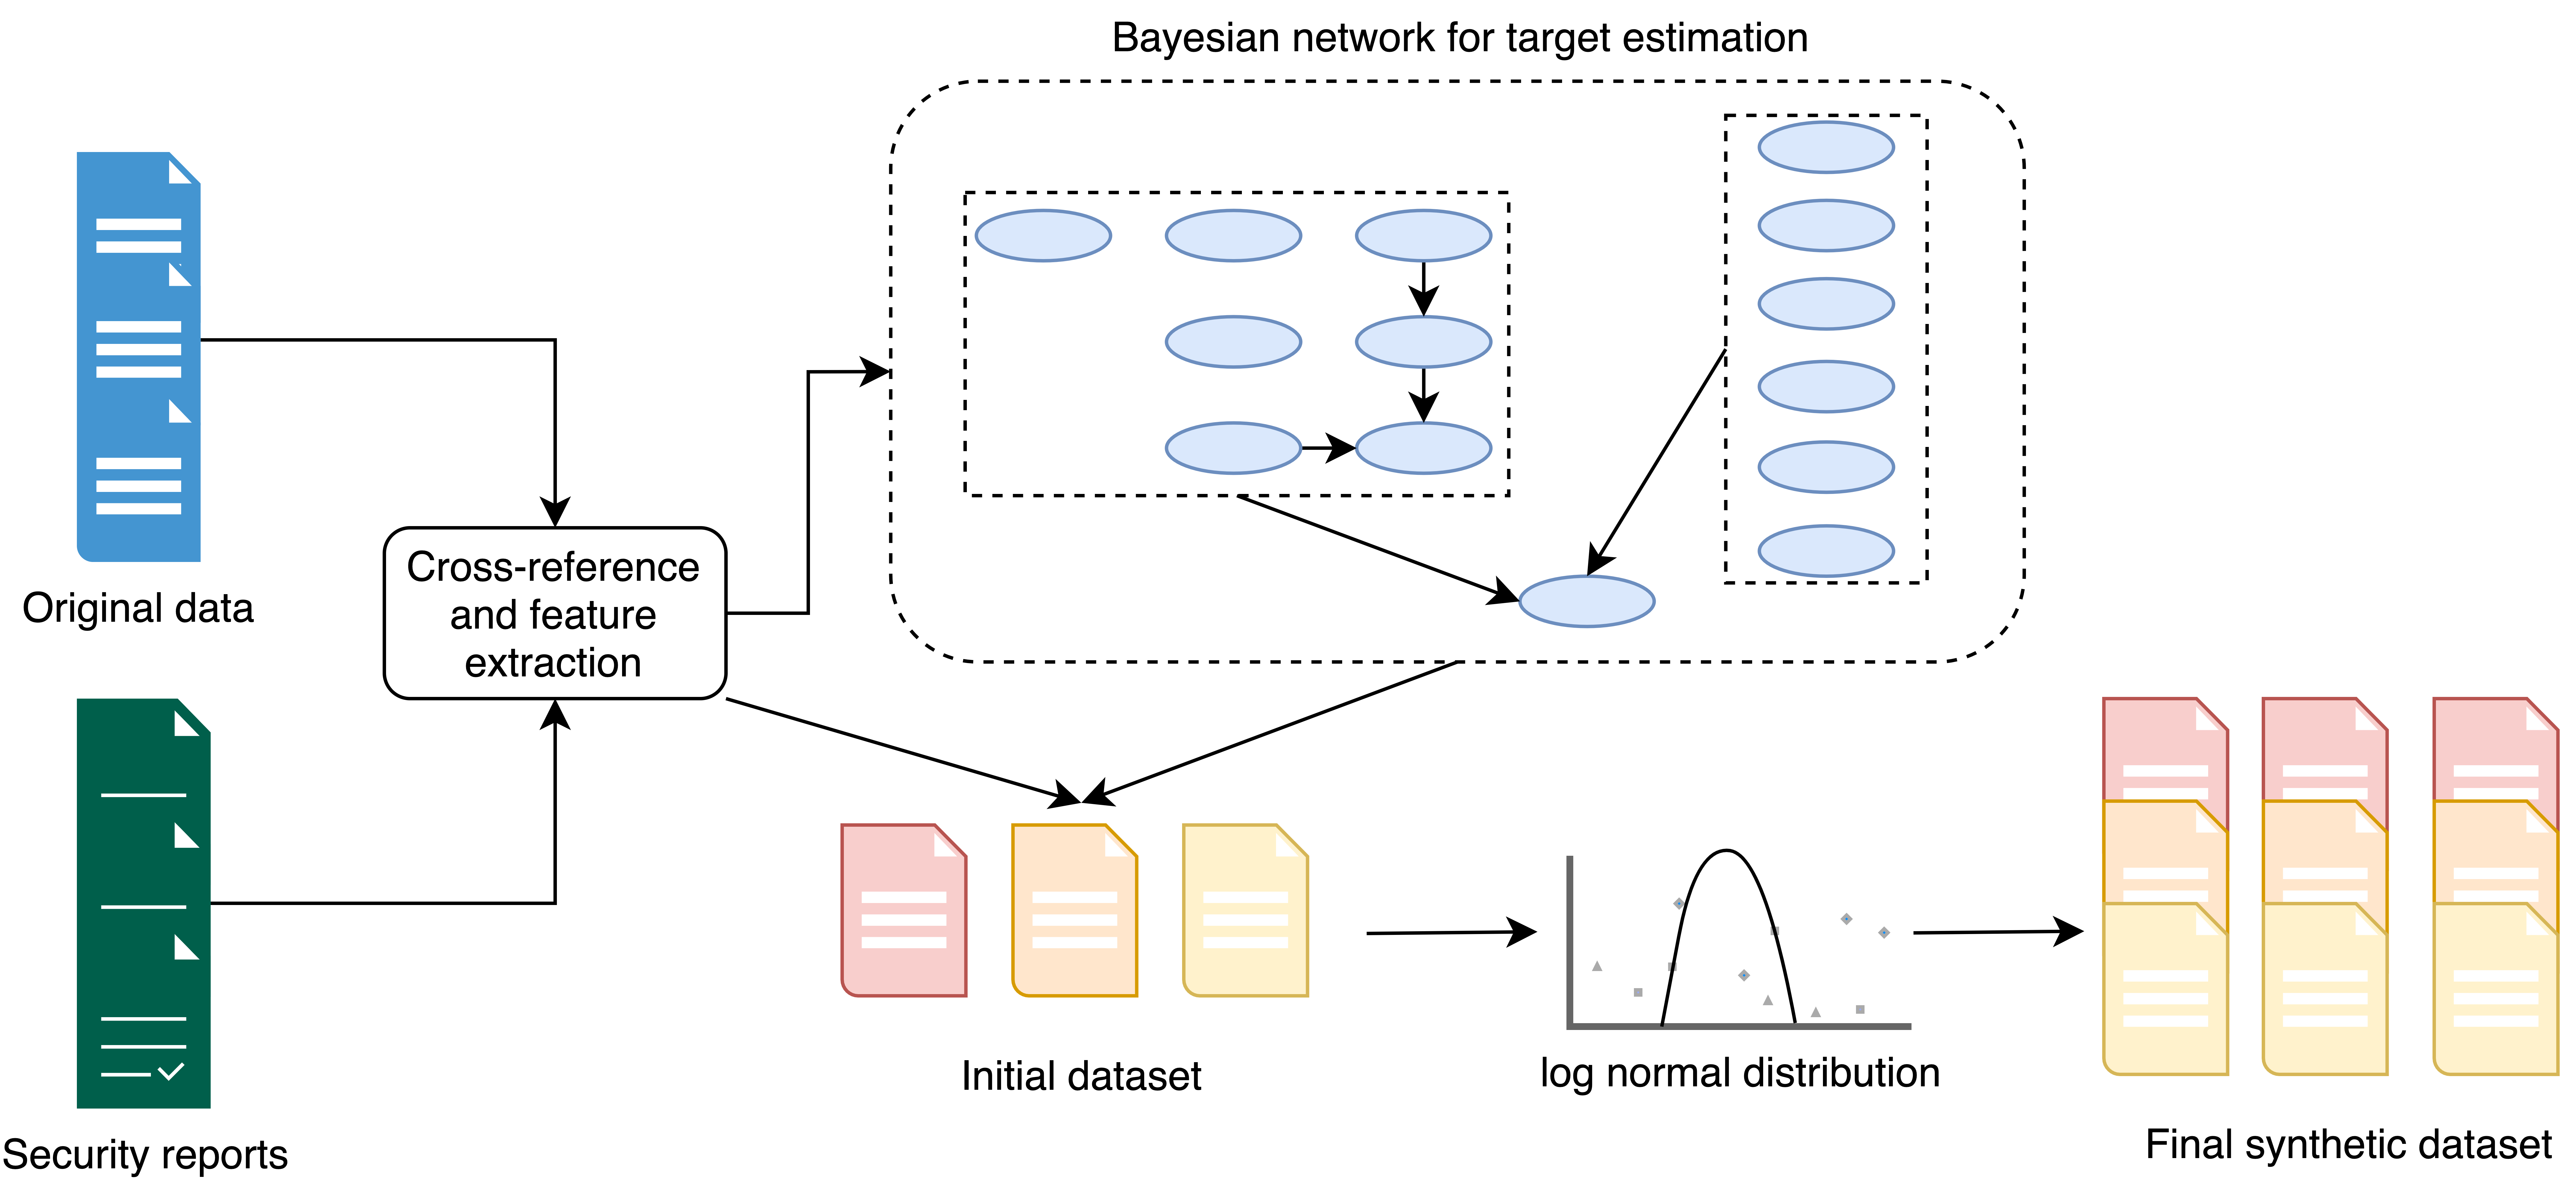
\includegraphics[scale=0.82]{images/synthetic/synthetic_data_complete}
	\caption{\label{fig:data_gen} Synthetic data generation process.}
\end{figure}

In a first part, we cross-reference the few questionnaires we were given with various security reports, and extract our dataset's features. This is presented in Section ~\ref{section:identify_feature}. In a second part, we build a Bayesian network based on the extracted features to estimate our dataset's targets. This is described in Section ~\ref{sec:target_estimation}. Finally, we use a log normal distribution to generate samples that share the same features but that have different target values. This is covered in Section ~\ref{section:generation}.  

\section{Features extraction}\label{section:identify_feature}

There are two components to any dataset: a set of features and a set of targets. The former describes attributes of the dataset's instances, while the latter captures the goal of the prediction task. The set of features and the set of targets should be closely related, otherwise the learning task becomes quite meaningless. Consider for instance the adult\footnote{\url{https://archive.ics.uci.edu/ml/datasets/adult}} dataset, where the prediction task is to determine whether or not a person makes over $50k$\$ a year. The set of features is composed of various attributes about the persons: their age, education, work-class, etc. These features are directly relevant to the prediction task, since they will influence the target value: a person that graduated high school versus a person that graduated from a Doctorate degree are likely to have a measurable income gap.


To identify our features, we need to understand how companies handle security, i.e. what are their security practices, and what are the implications on the \textit{loss} and \textit{cost} targets. These security practices can be technical (e.g. firewall configuration) or operational (e.g. does the company have a security and privacy policy that their employees must adhere to). Unfortunately, companies are likely to be concerned that honest answers indicating poor IT security practices could be used to discriminate against them. Hence, they are not very keen on releasing such information.

To shed some light on this, we went through annually released security reports from various vendors: Verizon \cite{verizon_report}, NetDiligence \cite{netdiligence_report}, IBM \cite{ibm_report}, Cisco \cite{cisco_report}, Checkpoint \cite{checkpoint_report}, and AIG \cite{aig_report}. These reports highlight current security practices that company follow (or, fail to follow) and provide insights about the threat landscape they face, in an anonymised fashion. Of particular relevance to our business problem, the NetDiligence \cite{netdiligence_report} and AIG \cite{aig_report} reports provide data from the insurer's perspective, highlighting common causes and consequences about cyber attacks that their clients suffered.

Using these reports, we can derive useful probabilities. NetDiligence \cite{netdiligence_report} shows that in the $2014-2018$ period, social engineering (act of tricking someone into divulging information or taking action) was responsible for 28\% of the claims they received from companies. Since this number is post-incident, we can transform it into a conditional probability between the event \textit{social engineering} and the event \textit{the company suffers a loss}: $Pr(social\_engineering | loss) = 0.28$. To benefit our synthetic data generation problem, we can tweak this a little and create a new feature, \textit{$f_1$ = company\_trains\_employees\_against\_social\_engineering}. We can now artificially derive: $Pr(f_1 | loss) = 1 - Pr(social\_engineering | loss) = 1 - 0.28 = 0.72$. It could be argued that for some companies, training was delivered but improperly, thus raising questions about the probability that was derived. For this thesis and for the sake of simplicity, we will assume an ideal scenario.

Following a similar approach, we derive multiple such features and probabilities across all the reports, which we summarise in Table ~\ref{table:probs}. If multiple vendors report about the same incident (e.g. social engineering), we take the mean value that was reported across all reports. As these reports do not provide pre-incident figures (e.g., $Pr(f_1)$), we manually assign a probability to such events, where relevant. We additionally create the following features for which the reports did not provide any information: \textit{company\_uses\_3rd\_party}, \textit{company\_has\_ids\_ips}, \textit{company\_has\_recovery\_plan}, \textit{company\_has\_firewalls}. For the company sector, we create a single feature \textit{sector} which can be one of $[hospitality, \; manufacturing, \; energy, \; \dots]$. We let the reader refer to Table ~\ref{table:features_meaning} for more information about the features and their meaning.

While the companies' security practices will likely influence the \textit{loss} target, not all features influence the \textit{cost} target. Typically, \textit{$f_1$ = social\_engineering} is not expected to contribute to the \textit{cost} target, as this target is post-incident: employees being trained against social engineering is not expected to influence how much the company will lose once an incident has happened. To make up the \textit{cost} target, we need to position ourselves on the attacker's side. Once an initial foothold inside the company has been established, the kind of data they may be able to find is likely to be relevant, as it will allow them to progress their attack further.

The Verizon report \cite{verizon_report} gives us a breakdown of the type of data that each industry is likely to possess: PII (personal identifiable information), PCI (payment card industry), PHI (protected health information), credentials (passwords), or 'other'. This is reported in Table ~\ref{table:probs-data}. This allows us to derive further features: \textit{company\_has\_pii, company\_has\_pci, company\_has\_phi, etc}.

\begin{center}\begin{table}[h!]
	\center
	\noindent\makebox[0pt]{}{
		\begin{tabular}{|c|c|c|c|c| } 
 		\hline
 		Feature ($F$) & $Pr(F)$ & $Pr(F | loss)$ & $Pr(F|SME)$ & $Pr(F| large)$ \\ [0.5ex] \hline\hline
 		$company\_is\_in\_hospitality$ & & & 0.03 & 0.04 \\ \hline
 		$company\_is\_a\_public\_entity$ & & & 0.03 & \\ \hline
 		$company\_is\_in\_other$ & & & 0.11 & 0.09 \\ \hline
 		$company\_is\_a\_nonprofit$ & & & 0.05 & \\ \hline
 		$company\_is\_in\_education$ & & & 0.05 & 0.08 \\ \hline
 		$company\_is\_in\_technology$ & & & 0.06 & 0.03\\ \hline
 		$company\_is\_in\_manufacturing$ & & & 0.08 & 0.03 \\ \hline
 		$company\_is\_in\_financial\_services$ & & & 0.09 & 0.15\\ \hline
 		$company\_is\_in\_energy$ & & & & 0.04 \\ \hline
 		$company\_is\_in\_retail$ & & & 0.09 & 0.24\\ \hline
 		$company\_is\_in\_healthcare$ & & & 0.19 & 0.26\\ \hline
 		$company\_is\_in\_professional\_services$ & & & 0.22 & 0.04 \\ \hline
 		\makecell{$company\_trains\_employees\_$\\$against\_social\_engineering$} & 0.70 & 0.8025 & & \\ \hline
 		$company\_has\_patching\_process$ & 0.60 & 0.828 & & \\ \hline
 		$company\_has\_antivirus$ & 0.95 & 0.81 & & \\ \hline
 		$company\_uses\_3rd\_party$ & 0.87 & & & \\ \hline
 		$company\_has\_ids\_ips$ & 0.94 & & & \\ \hline
 		$company\_has\_recovery\_plan$ & 0.33 & & & \\ \hline
 		$company\_has\_firewalls$ & 0.83 & & & \\ \hline
	\end{tabular}
	\caption{\label{table:probs} Potential features for the synthetic dataset and their respective probabilities. We separate small and medium sized businesses (SME) from large businesses.}}
\end{table}\end{center}

\begin{center}\begin{table}[h!]
	\center
	\noindent\makebox[0pt]{}{
		\begin{tabular}{|c|c|c|c|c|c|} 
 		\hline
 		Sector ($S$) & $Pr(PII | S)$ & $Pr(PCI|S)$ & $Pr(PHI|S)$ & $Pr(credentials|S)$ & $Pr(other|S)$ \\ [0.5ex] \hline\hline
 		$Hospitality$ & 0.44 & & & 0.34 & 0.23 \\ \hline
 		$Public \; Entity$ & 0.51 & & & 0.33 & 0.34\\ \hline
 		$Other$ & 0.81 & & & 0.36 & 0.42 \\ \hline
 		$Education$ & 0.75 & & & 0.30 & 0.23 \\ \hline
 		$Technology$ & 0.69 & & & 0.41 & 0.34 \\ \hline
 		$Manufacturing$ & 0.49 & 0.20 & & 0.55 & 0.25 \\ \hline
 		$Financial \; Services$ & 0.77 & 0.32 & & 0.35 & 0.35 \\ \hline
 		$Energy$ & 0.41 & 0.68 & & 0.41 & 0.35 \\ \hline
 		$Retail$ & 0.49 & 0.47 & & 0.27 & 0.25 \\ \hline
 		$Healthcare$ & 0.77 & & 0.67 & 0.18 & 0.18 \\ \hline
 		$Professional \; Services$ & 0.75 & & & 0.45 & 0.32 \\ \hline
	\end{tabular}
	\caption{\label{table:probs-data} Probabilities for companies within a specific sector to store a certain type of data}}
\end{table}\end{center}

\section{Targets estimation}\label{sec:target_estimation}

Section ~\ref{section:identify_feature} introduced a way to identify the set of features for our synthetic dataset, and their corresponding probabilities for feature selection. Feature selection consists in deciding if a feature is \textit{True} or \textit{False} for a given company. For instance, the social engineering feature $f_1$ has a probability of $Pr(f_1) = 0.70$ according to Table ~\ref{table:probs}. During the data generation process, each instance will see this feature set to \textit{True} with probability 0.70, and to \textit{False} with probability 0.30. This process of feature selection is repeated across all features. Once this is done, we must use the results of the feature selection process to compute fictive values for our targets \textit{loss} and \textit{cost}. This section presents two approaches, both using Bayesian networks, that vary in complexity.


\begin{definition}[Graphical model \cite{bayes}]
	A graphical model is a tool that is used to visually illustrate and work with conditional independencies among variables in a given problem.
\end{definition}

A graph is composed of a set of nodes (which represent the variables) and a set of edges. Each edge connects two nodes, and an edge can have an optional direction associated to it. Two variables are conditionally independent if they have no direct impact on each other's value. Figure ~\ref{fig:graph_model} shows an example of a graphical model.

\begin{figure}[h!]
	\center
	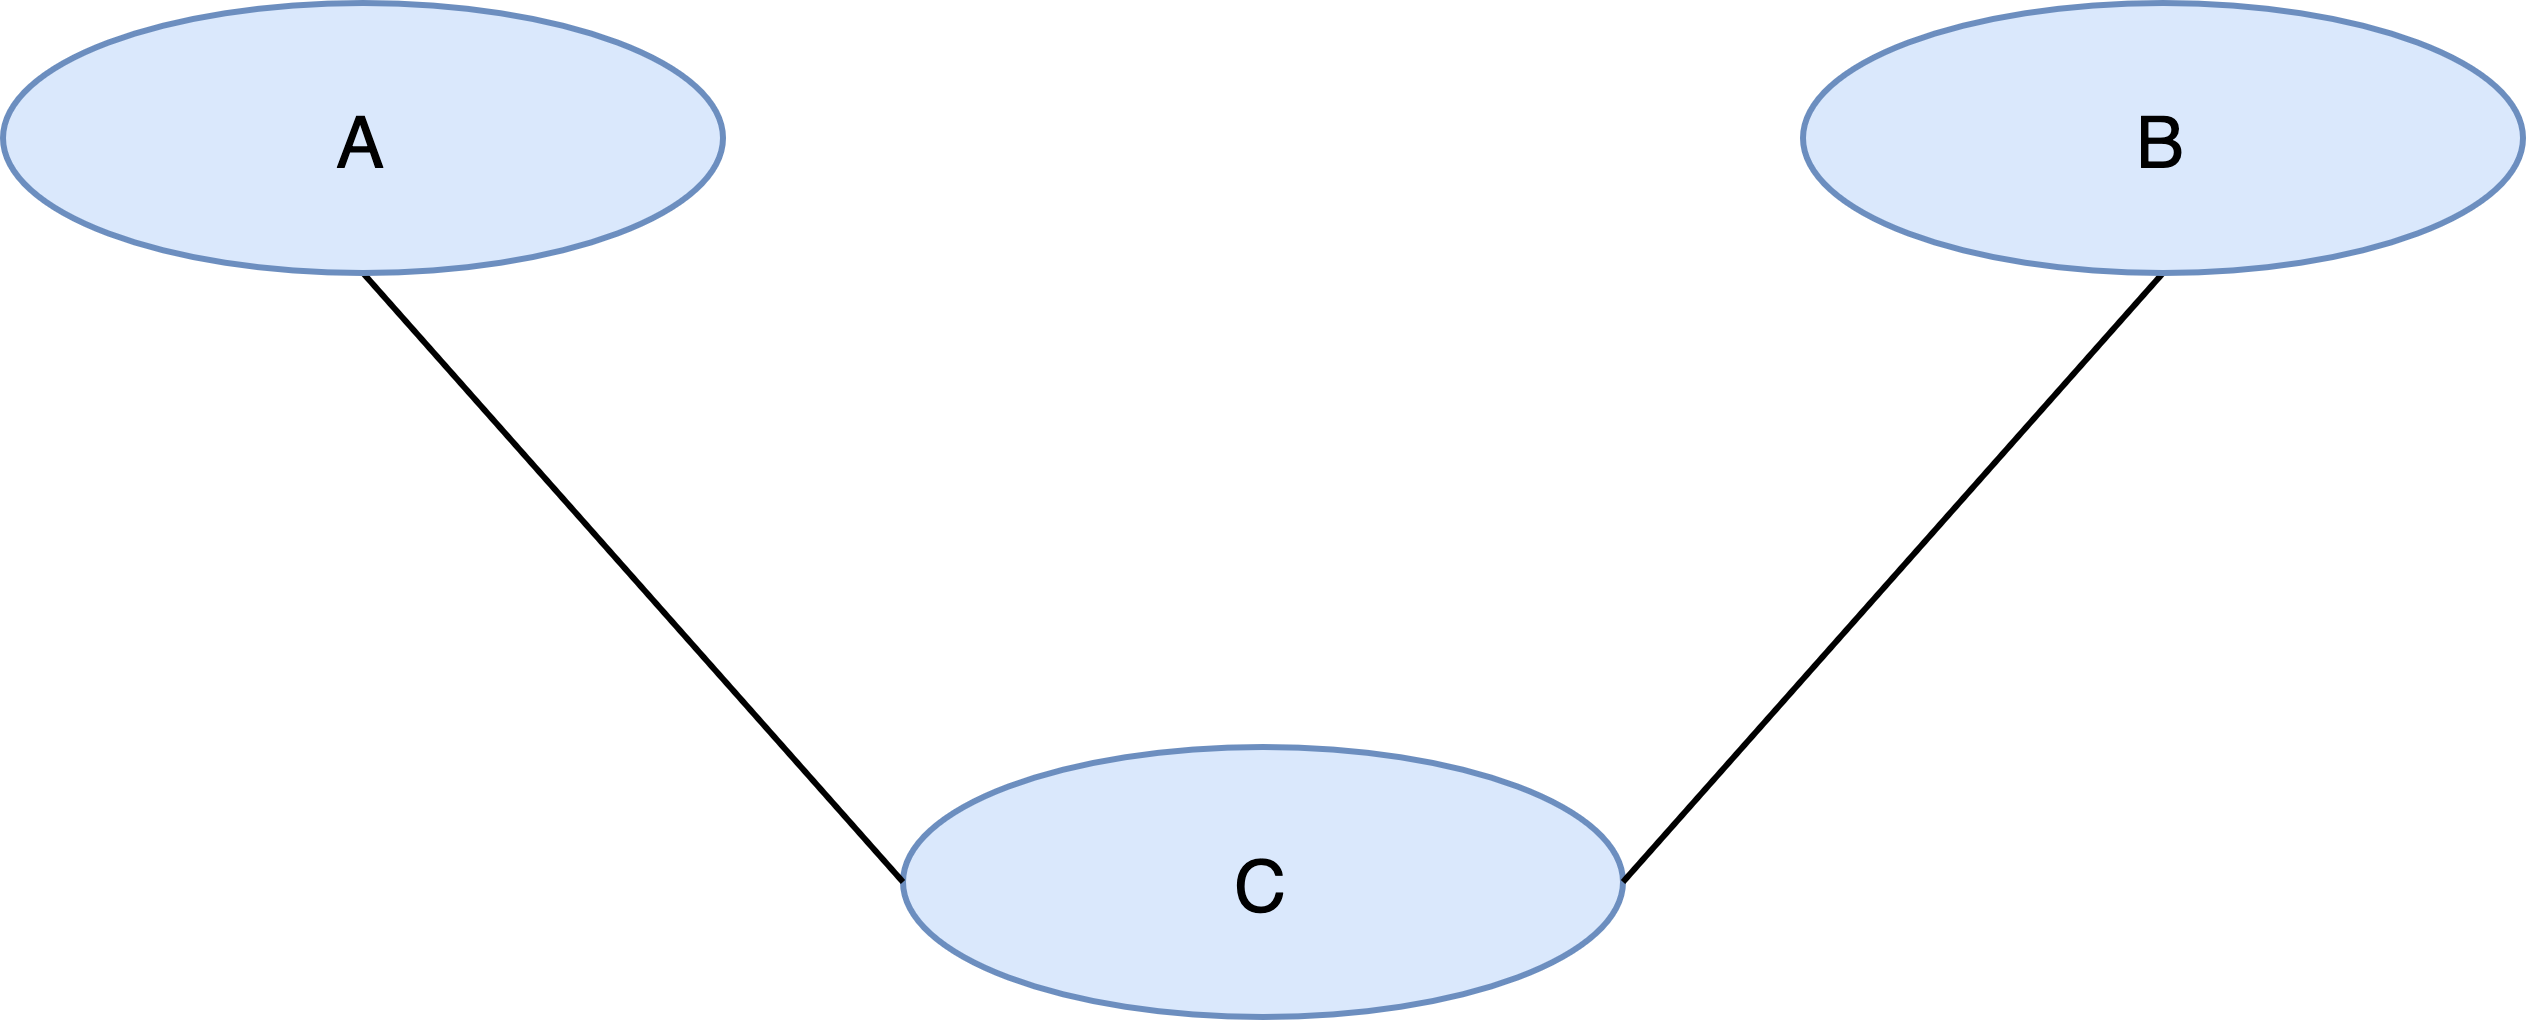
\includegraphics[scale=0.63]{images/synthetic/graphical_model.png}
	\caption{\label{fig:graph_model} A graphical mode,  in which A and B are conditionally independent given C.}
\end{figure}

\begin{definition}[Bayesian network \cite{bayes}]
	Bayesian networks are a particular instance of graphical models. They are directed acyclic graphs (DAG): all edges in the graph are directed (i.e. they point in a particular direction) and there are no cycles (i.e. there is no way to start from a node, travel along a set of directed edges and arrive back at the starting node).
\end{definition}

Figure ~\ref{fig:bayesian} illustrates a Bayesian network. Given nodes $\textbf{X} = X_1, \dots, X_n$, the joint probability function for any Bayesian network is $Pr(\textbf{X}) = \prod_{i=1}^nPr(X_i | parents(X_i))$. This means that the joint probability of all the variables is the product of the probabilities of each variable given its parents' value. In Figure ~\ref{fig:bayesian}, we have $Pr(A,B,C) = Pr(A)Pr(B)Pr(C|A,B)$.

\begin{figure}[h!]
	\center
	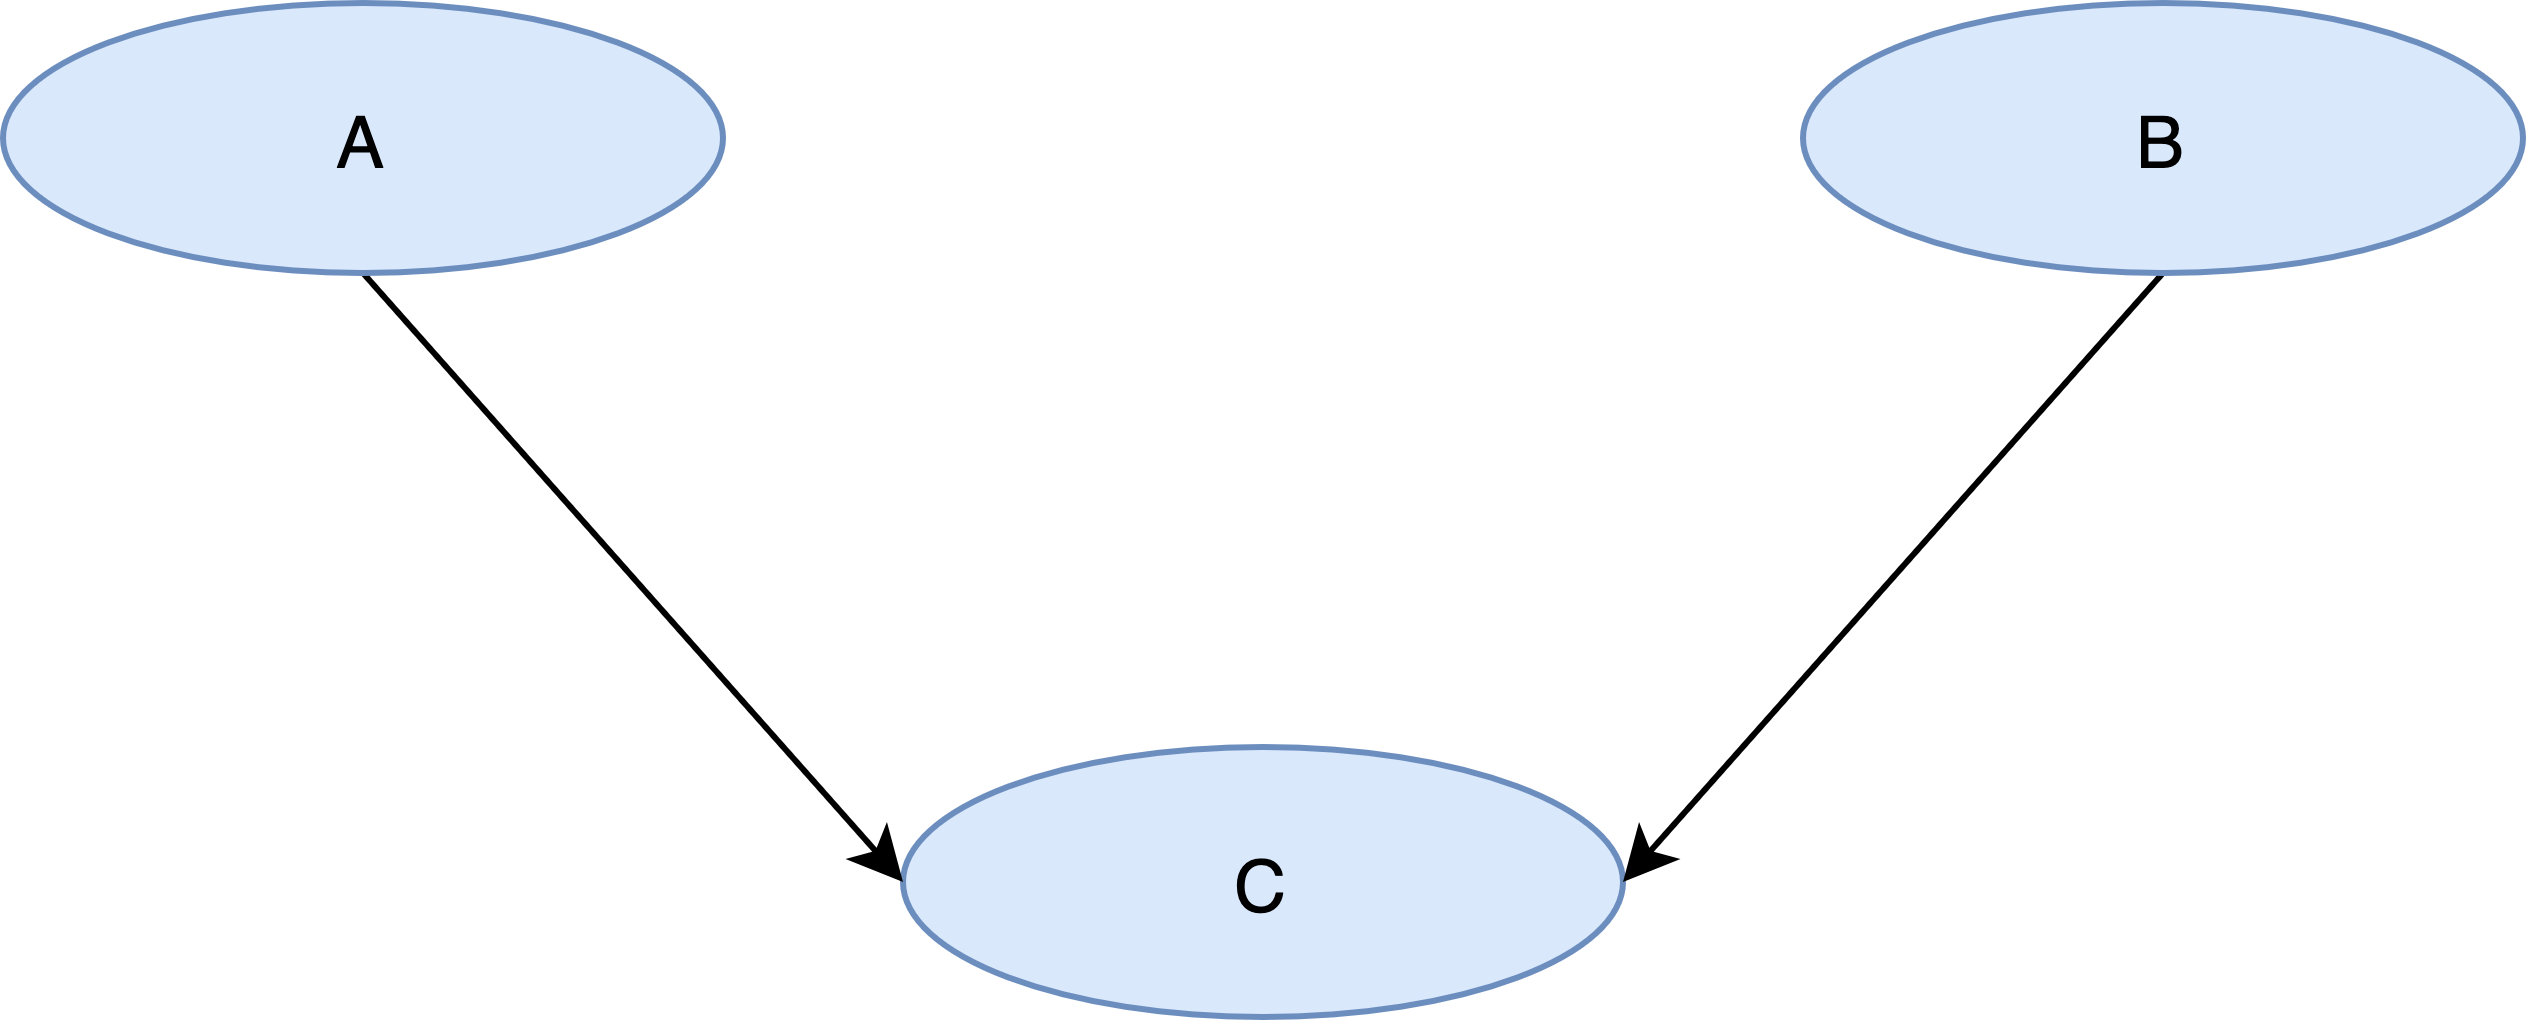
\includegraphics[scale=0.63]{images/synthetic/bayesian.png}
	\caption{\label{fig:bayesian} A simple Bayesian network.}
\end{figure}

\subsection{Approach 1}

\subsubsection{Loss target}

For the \textit{loss} target, we propose the Bayesian network outlined in Figure ~\ref{fig:bayesian-easy}. We make the \textit{loss} target depend on a subset of the features: \textit{social engineering training}, \textit{antivirus}, and \textit{outdated software patching process}. Since the reports do not mention any correlations between these features, we assume that they are conditionally independent with respect to \textit{loss}.

\begin{figure}[h!]
	\center
	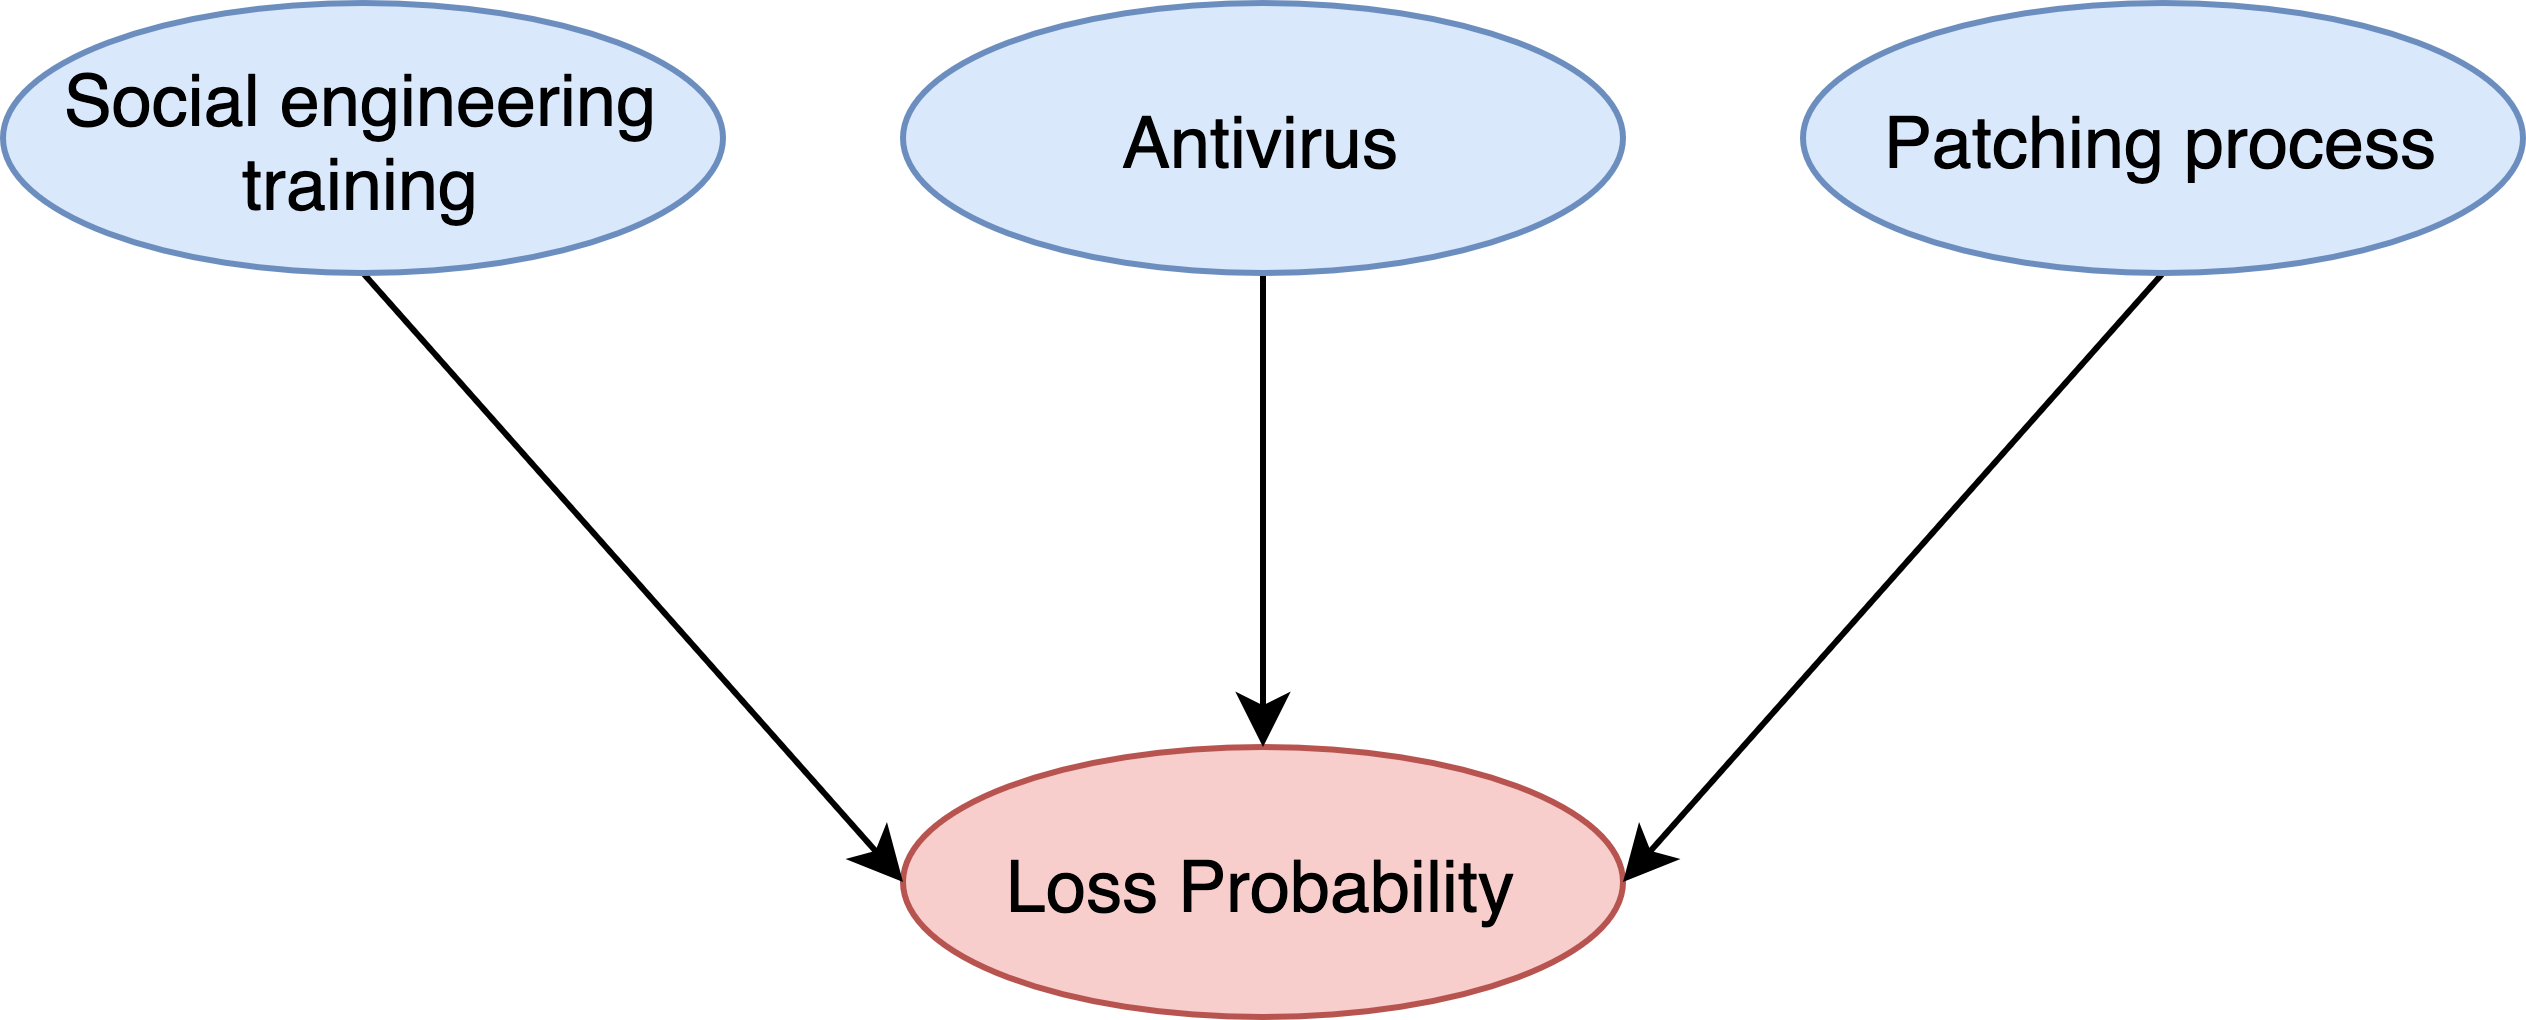
\includegraphics[scale=0.63]{images/synthetic/bayesian_easy}
	\caption{\label{fig:bayesian-easy} Bayesian network for the \textit{loss} target.}
\end{figure}

We can then derive: 

\begin{equation} \label{eq1}
\begin{split}
Pr(loss | social, antivirus, patching) & = \frac{Pr(loss, social, antivirus, patching)}{Pr(social)Pr(antivirus)Pr(patching)} \\
 & = \frac{Pr(social, antivirus, patching | loss)Pr(loss)}{Pr(social)Pr(antivirus)Pr(patching)} \\
 & = \frac{Pr(social|loss)Pr(antivirus|loss)Pr(patching|loss)}{Pr(social)Pr(antivirus)Pr(patching)}
\end{split}
\end{equation}

Fixing $Pr(loss) = 0.10$ and plugging in the data provided in Table ~\ref{table:probs}, we can compute the \textit{loss} target.

\subsubsection{Cost target}

To derive a number for the target \textit{cost}, we exclusively rely on data provided in the NetDiligence \cite{netdiligence_report} report:

\begin{itemize}
	\item The \texttt{min}, \texttt{max} and \texttt{mean} cost of a breach in a particular industry: $min(cost_{breach})$, $max(cost_{breach})$, $mean(cost_{breach})$
	\item The \texttt{mean} post-incident (crisis) cost, i.e. the breach remediation cost $cost_{remediation}$
	\item The \texttt{mean} cost per type of data that was potentially exposed, $cost_{data}$. This cost directly depends on the features of a given instance: if the instance is in healthcare, then as per Table ~\ref{table:probs-data}, we will add together the costs for leaked PII, PHI, credentials and others if these attributes are \textit{True} for that instance.
\end{itemize}

In particular, we derive the cost as per the following formula: $cost = triangular(min(cost_{breach}),$ $max(cost_{breach}), mean(cost_{breach})) + cost_{remediation} + \sum_{data}{cost_{data}}$ where $triangular()$ is the triangular distribution. Fig. ~\ref{fig:distribution-easy} shows the distribution of values for the targets over 1 million generated samples. The method used to generate the samples is detailed in Section ~\ref{section:generation}.

\begin{figure}[h!]
	\center
	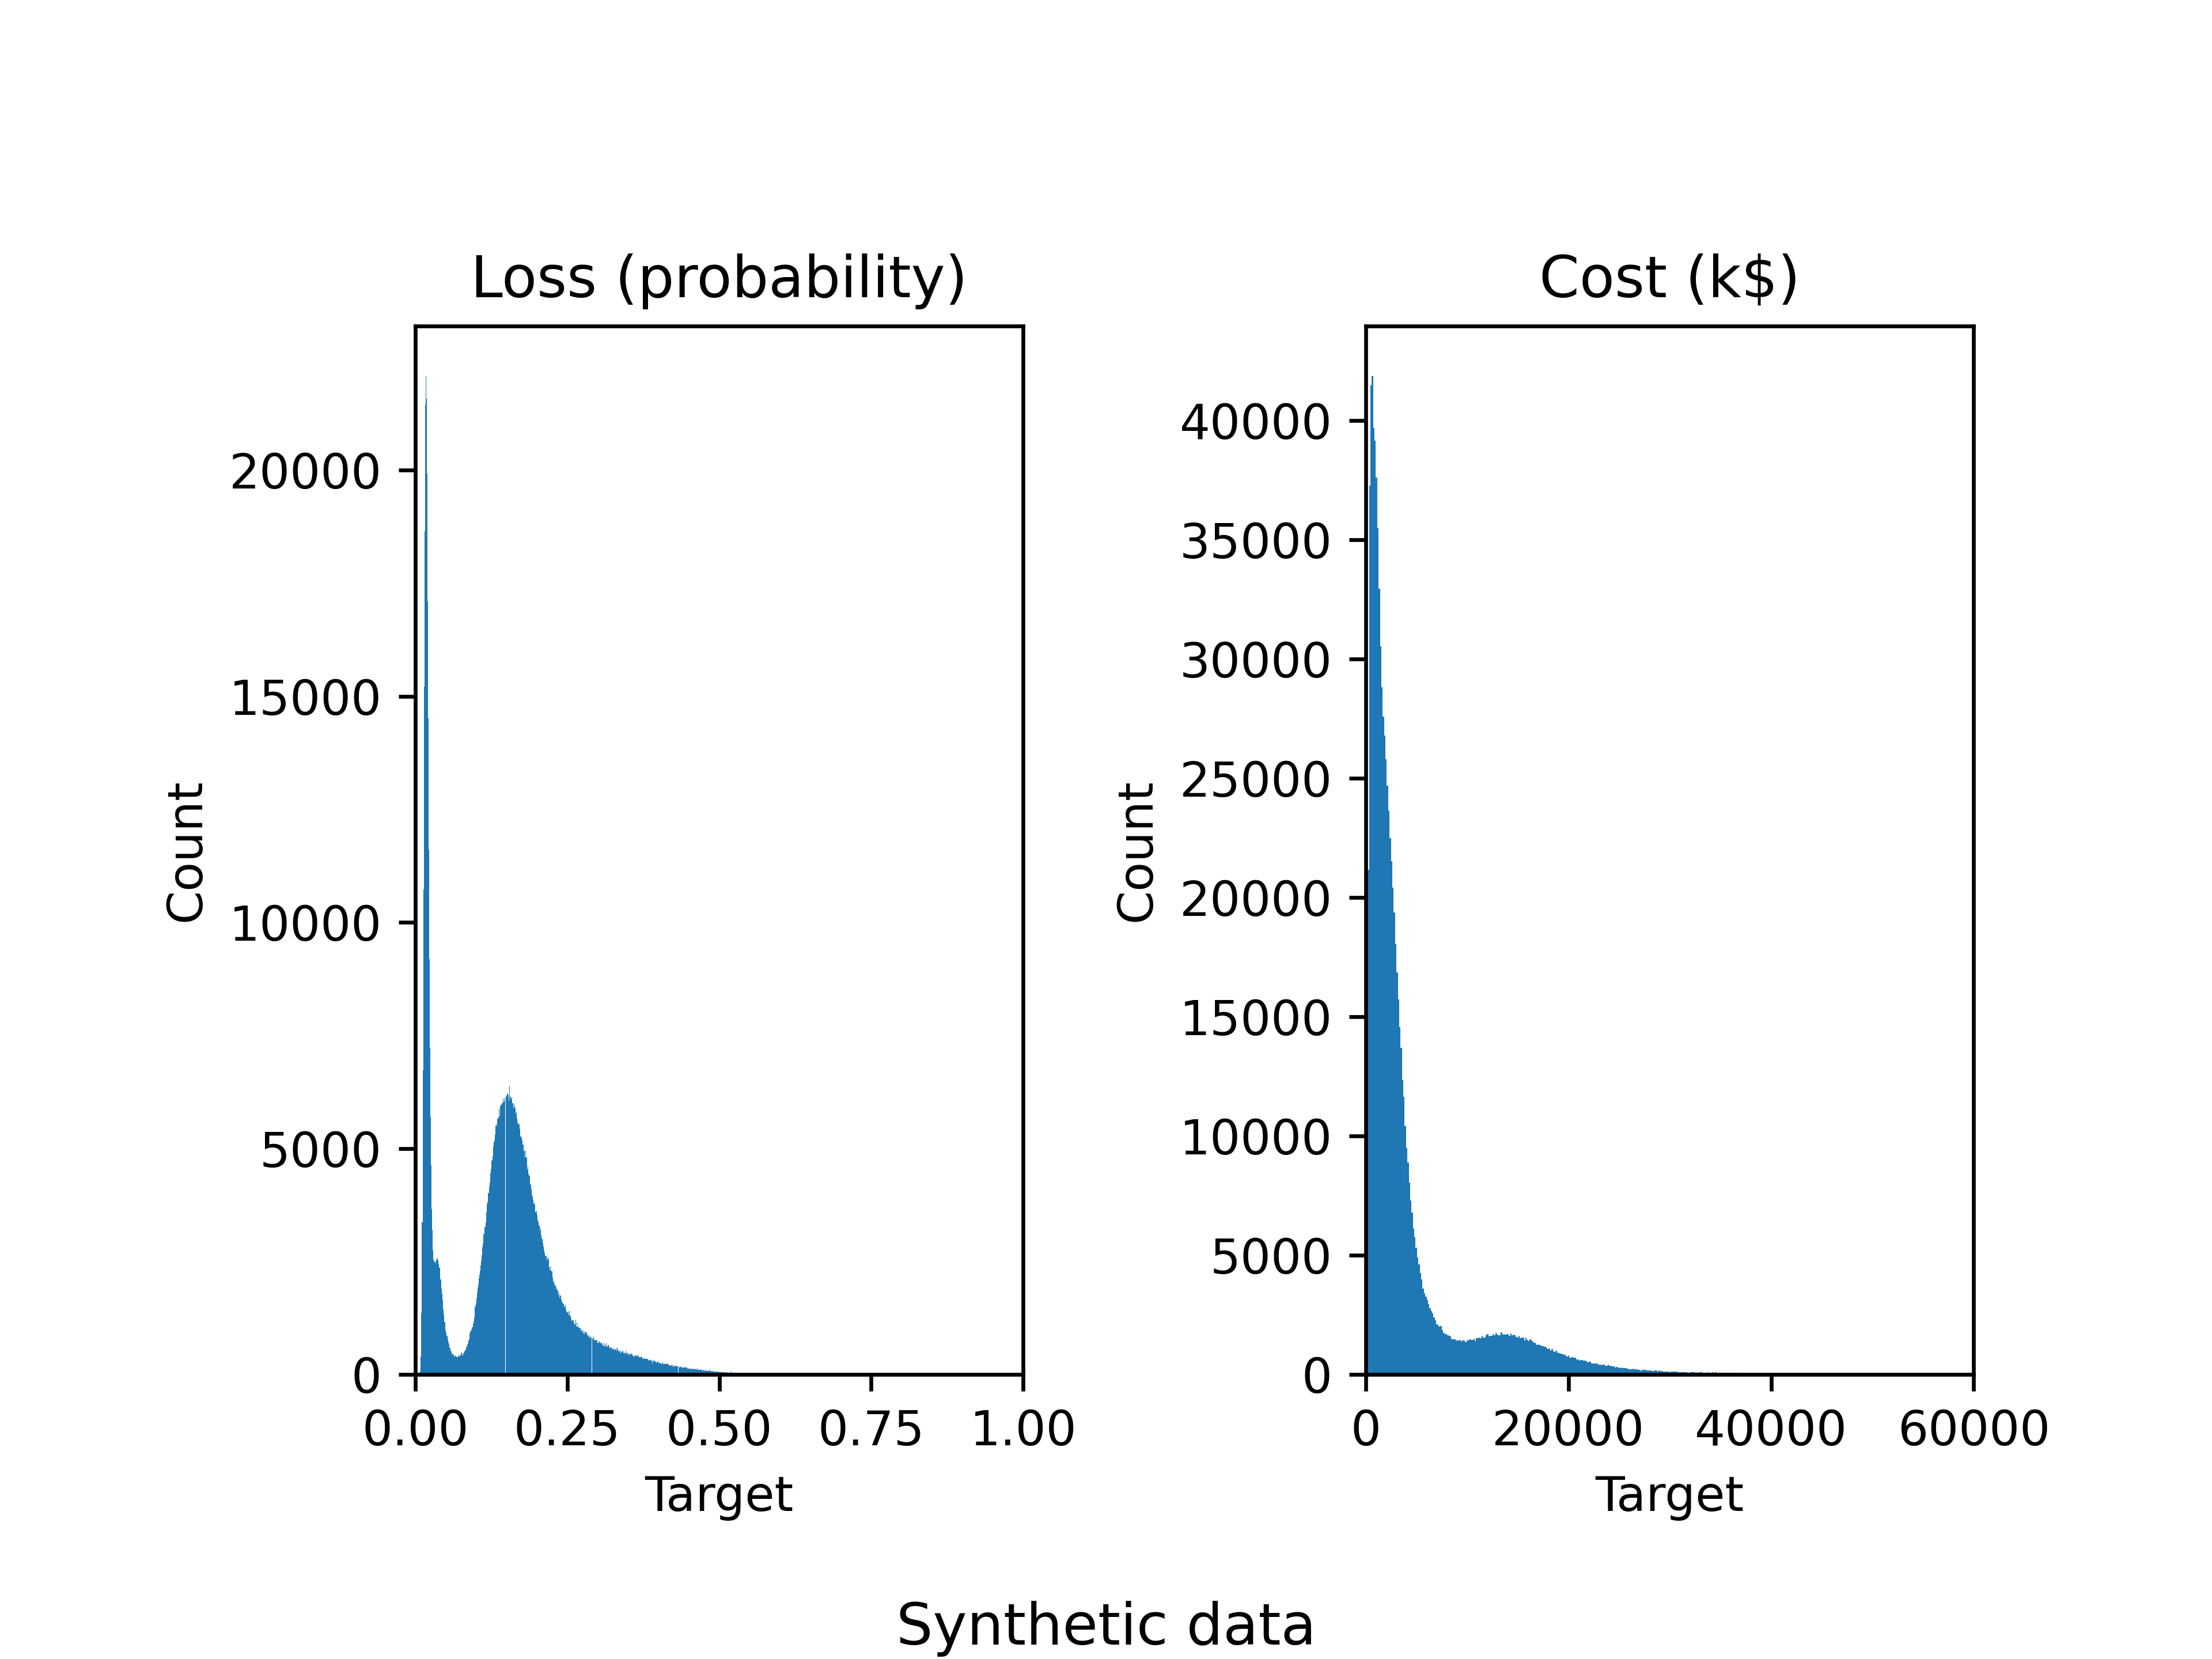
\includegraphics[scale=0.51]{images/synthetic/easy_distribution.png}
	\caption{\label{fig:distribution-easy} Target distribution for the synthetic dataset.}
\end{figure}

Unfortunately, our testing demonstrated that the problem was rendered hard through too much randomness / noise addition, rather than by the intricacies of the features and the targets themselves. This is why we now propose a second approach to the problem.

\subsection{Approach 2}

\subsubsection{Loss target}\label{subsubsection:prob_loss}

For the \textit{loss} target, we propose a more complex Bayesian network, as depicted in Figure ~\ref{fig:bayesian-hard}. Table ~\ref{table:all_probs} summarises the probabilities that we used in this model. Following the logic of Equation ~\ref{eq1}, we can derive:

\begin{figure}[h!]
	\center
	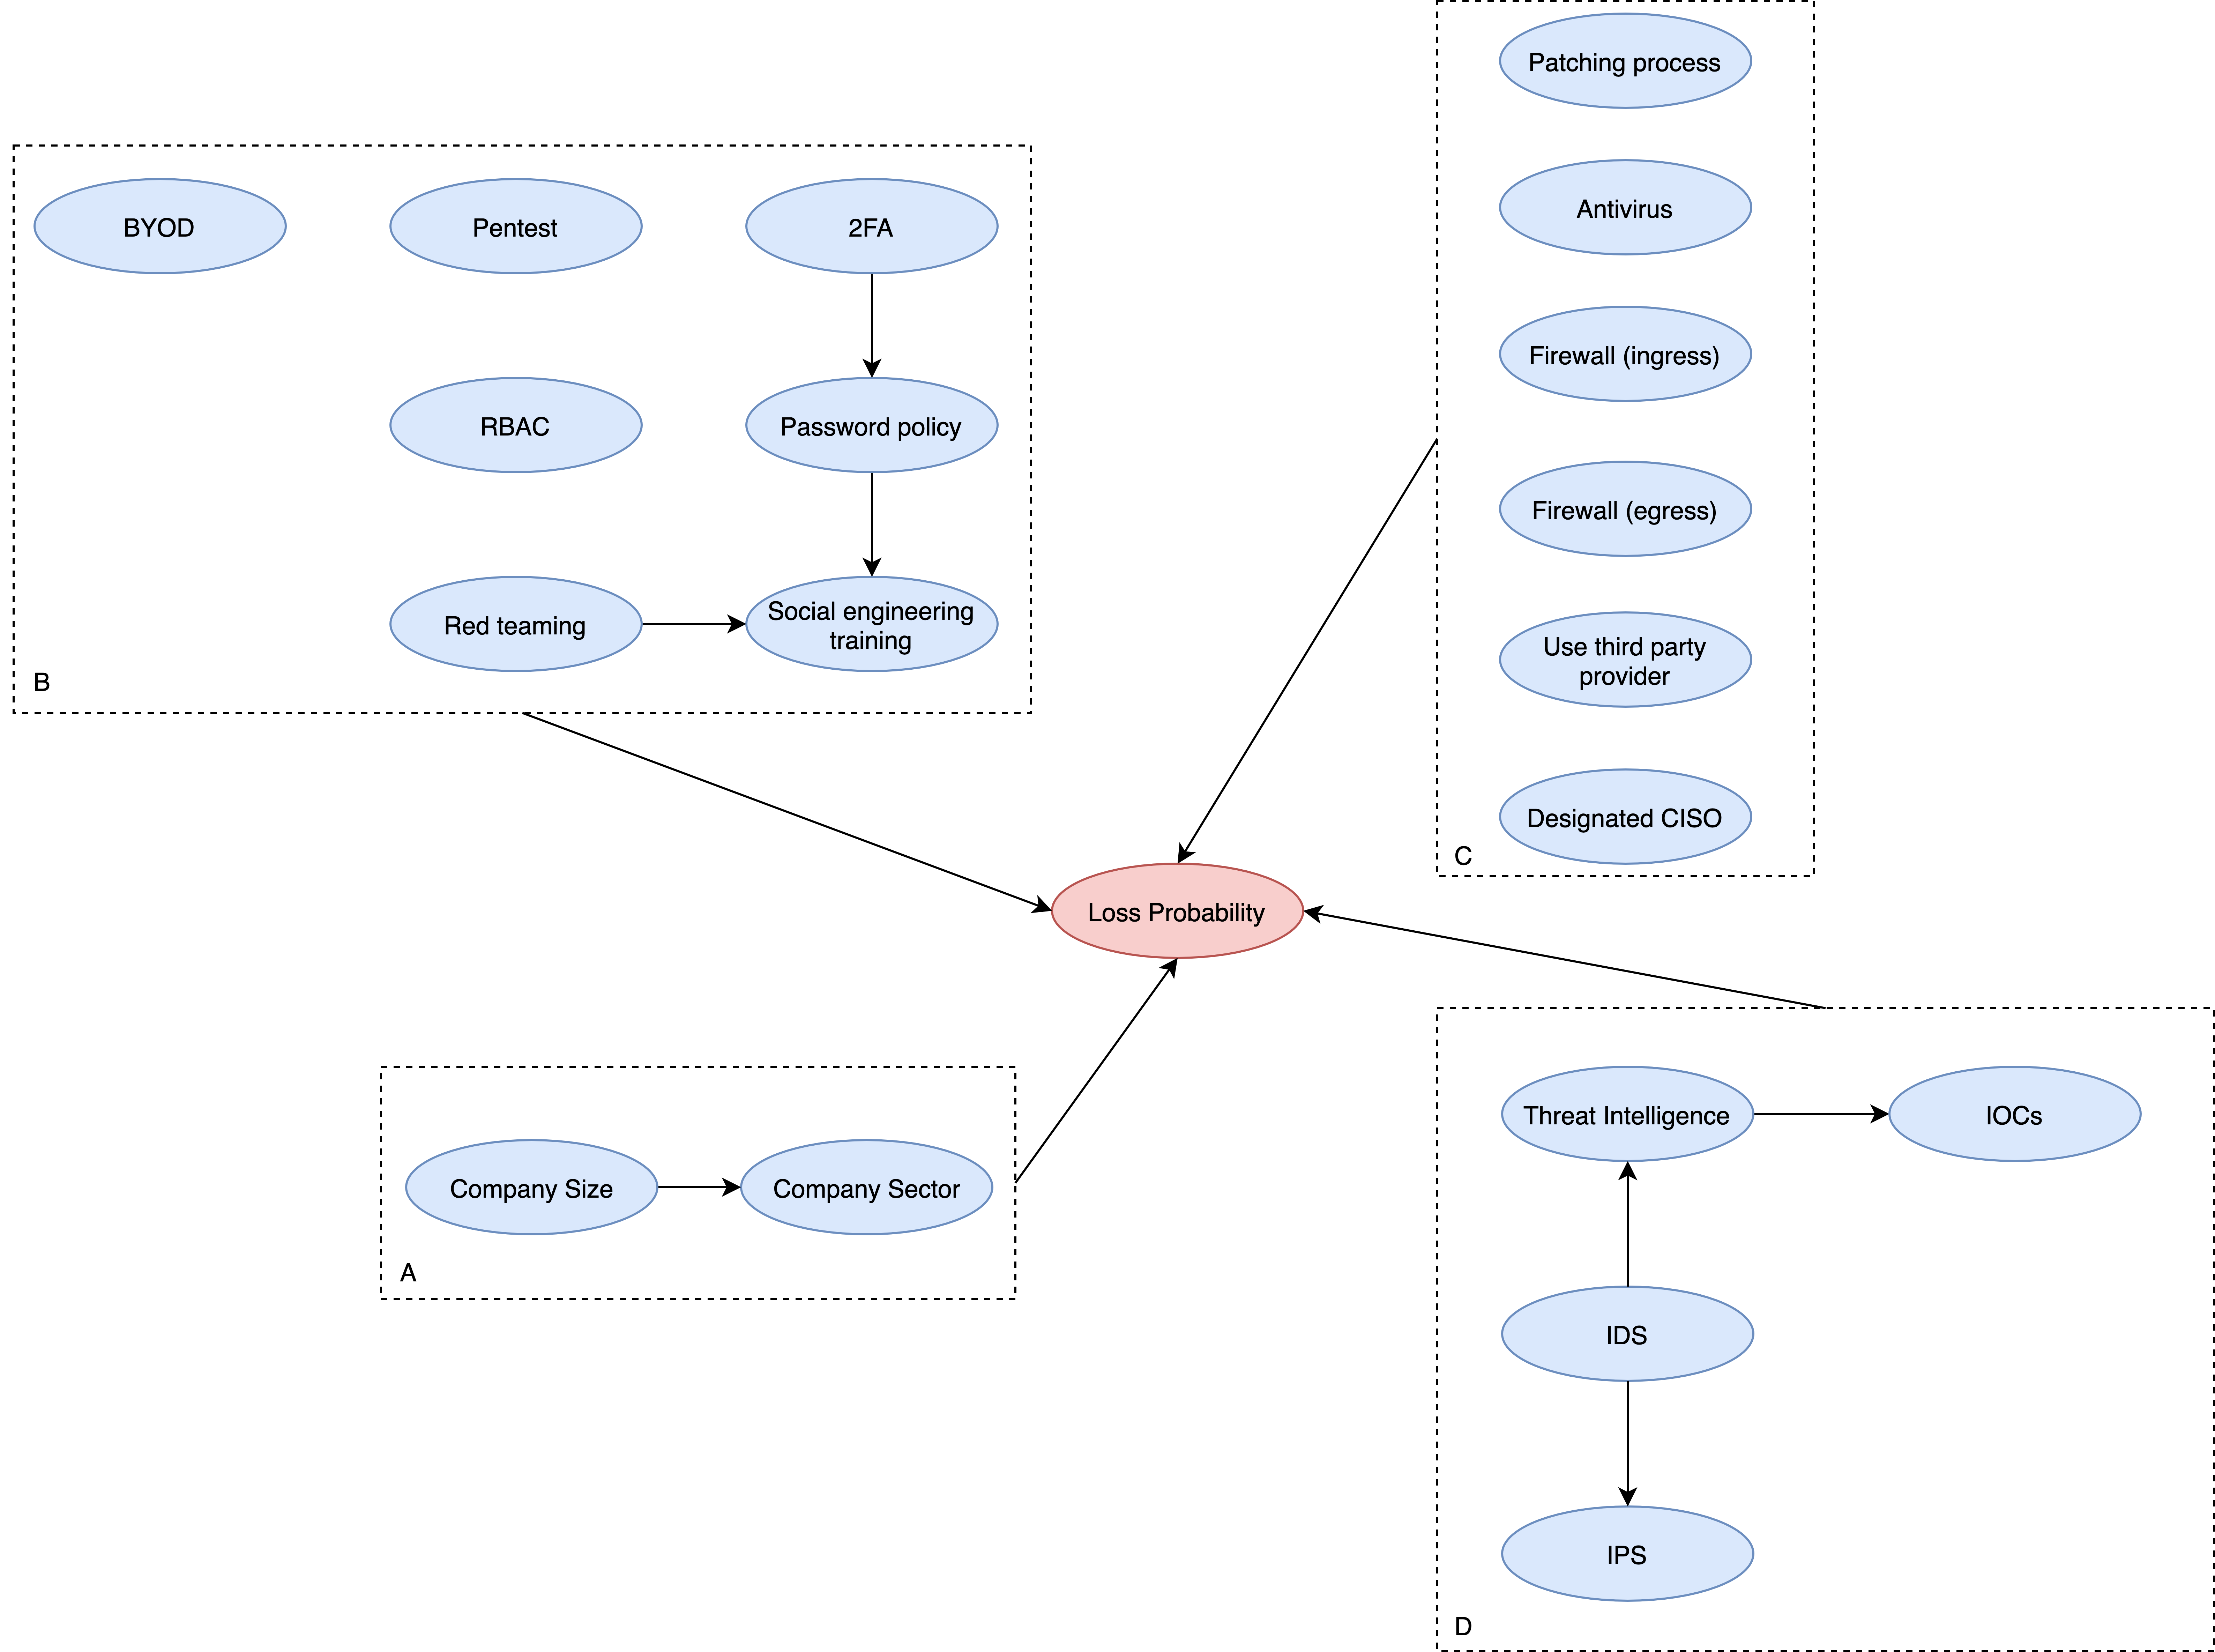
\includegraphics[scale=0.60]{images/synthetic/bayesian_hard.png}
	\caption{\label{fig:bayesian-hard} Revisited Bayesian network for the \textit{loss} target.}
\end{figure}

\begin{equation} \label{eq2}
\begin{aligned}
\begin{split}
Pr(A) & = Pr(company\_size | company\_sector)Pr(company\_size) \\
Pr(A|loss) & = Pr(company\_size, company\_sector | loss) \\
Pr(B) & = {Pr(BYOD)Pr(pentest)Pr(RBAC)Pr(red\_teaming)Pr(2FA)Pr(pwd\_policy | 2FA)}\\ 
& \ \ \ \ Pr(social|pwd\_policy,red\_teaming) \\
Pr(B|loss) & = Pr(BYOD|loss)Pr(pentest|loss)\\
& \ \ \ \ \ Pr(RBAC|loss)Pr(red\_teaming, 2FA, pwd\_policy,soc|loss) \\
Pr(C) & = Pr(patching)Pr(antivirus)Pr(fw\_ingress)Pr(fw\_egress)Pr(3rd\_party)Pr(CISO)\\
Pr(C|loss) & = Pr(patching|loss)Pr(antivirus|loss)Pr(fw\_ingress|loss)Pr(fw\_egress|loss) \\
& \ \ \ \ \ Pr(3rd\_party|loss)Pr(CISO|loss) \\
Pr(D) & = Pr(IPS|IDS)Pr(IDS)Pr(threat|IDS)Pr(IOC|threat) \\
Pr(D|loss) & = Pr(IPS, IDS, threat, IOC|loss)
\end{split}
\end{aligned}
\end{equation}

Which we can plug into:

\begin{equation} \label{eq6}
\begin{split}
Pr(loss|A,B,C,D) = \frac{Pr(A|loss)Pr(B|loss)Pr(C|loss)Pr(D|loss)Pr(loss)}{Pr(A)Pr(B)Pr(C)Pr(D)}
\end{split}
\end{equation}

\subsubsection{Cost target}\label{subsubsection:cost_calc}

For the \textit{cost} target, we propose additional features that influence the outcome, as shown in Figure ~\ref{fig:cost}. The cost is now computed as:

\begin{equation}\label{eq7}
	cost = \sum_{data}{cost_{data}} + \lambda_1mean(cost_{breach}) + \lambda_2cost_{remediation}
\end{equation}
where $\lambda_1$ and $\lambda_2$ $\in [0, 1]$ represent the fraction of the cost that should be applied to the instance. They are computed at runtime depending on the instance's features. For example, if the instance has the feature \textit{company\_has\_incident\_response\_team} set to \textit{True}, then we decrease $\lambda_2$ by a certain amount, as we expect the remediation cost to be lower in the presence of an IR team.

\begin{figure}[h!]
	\center
	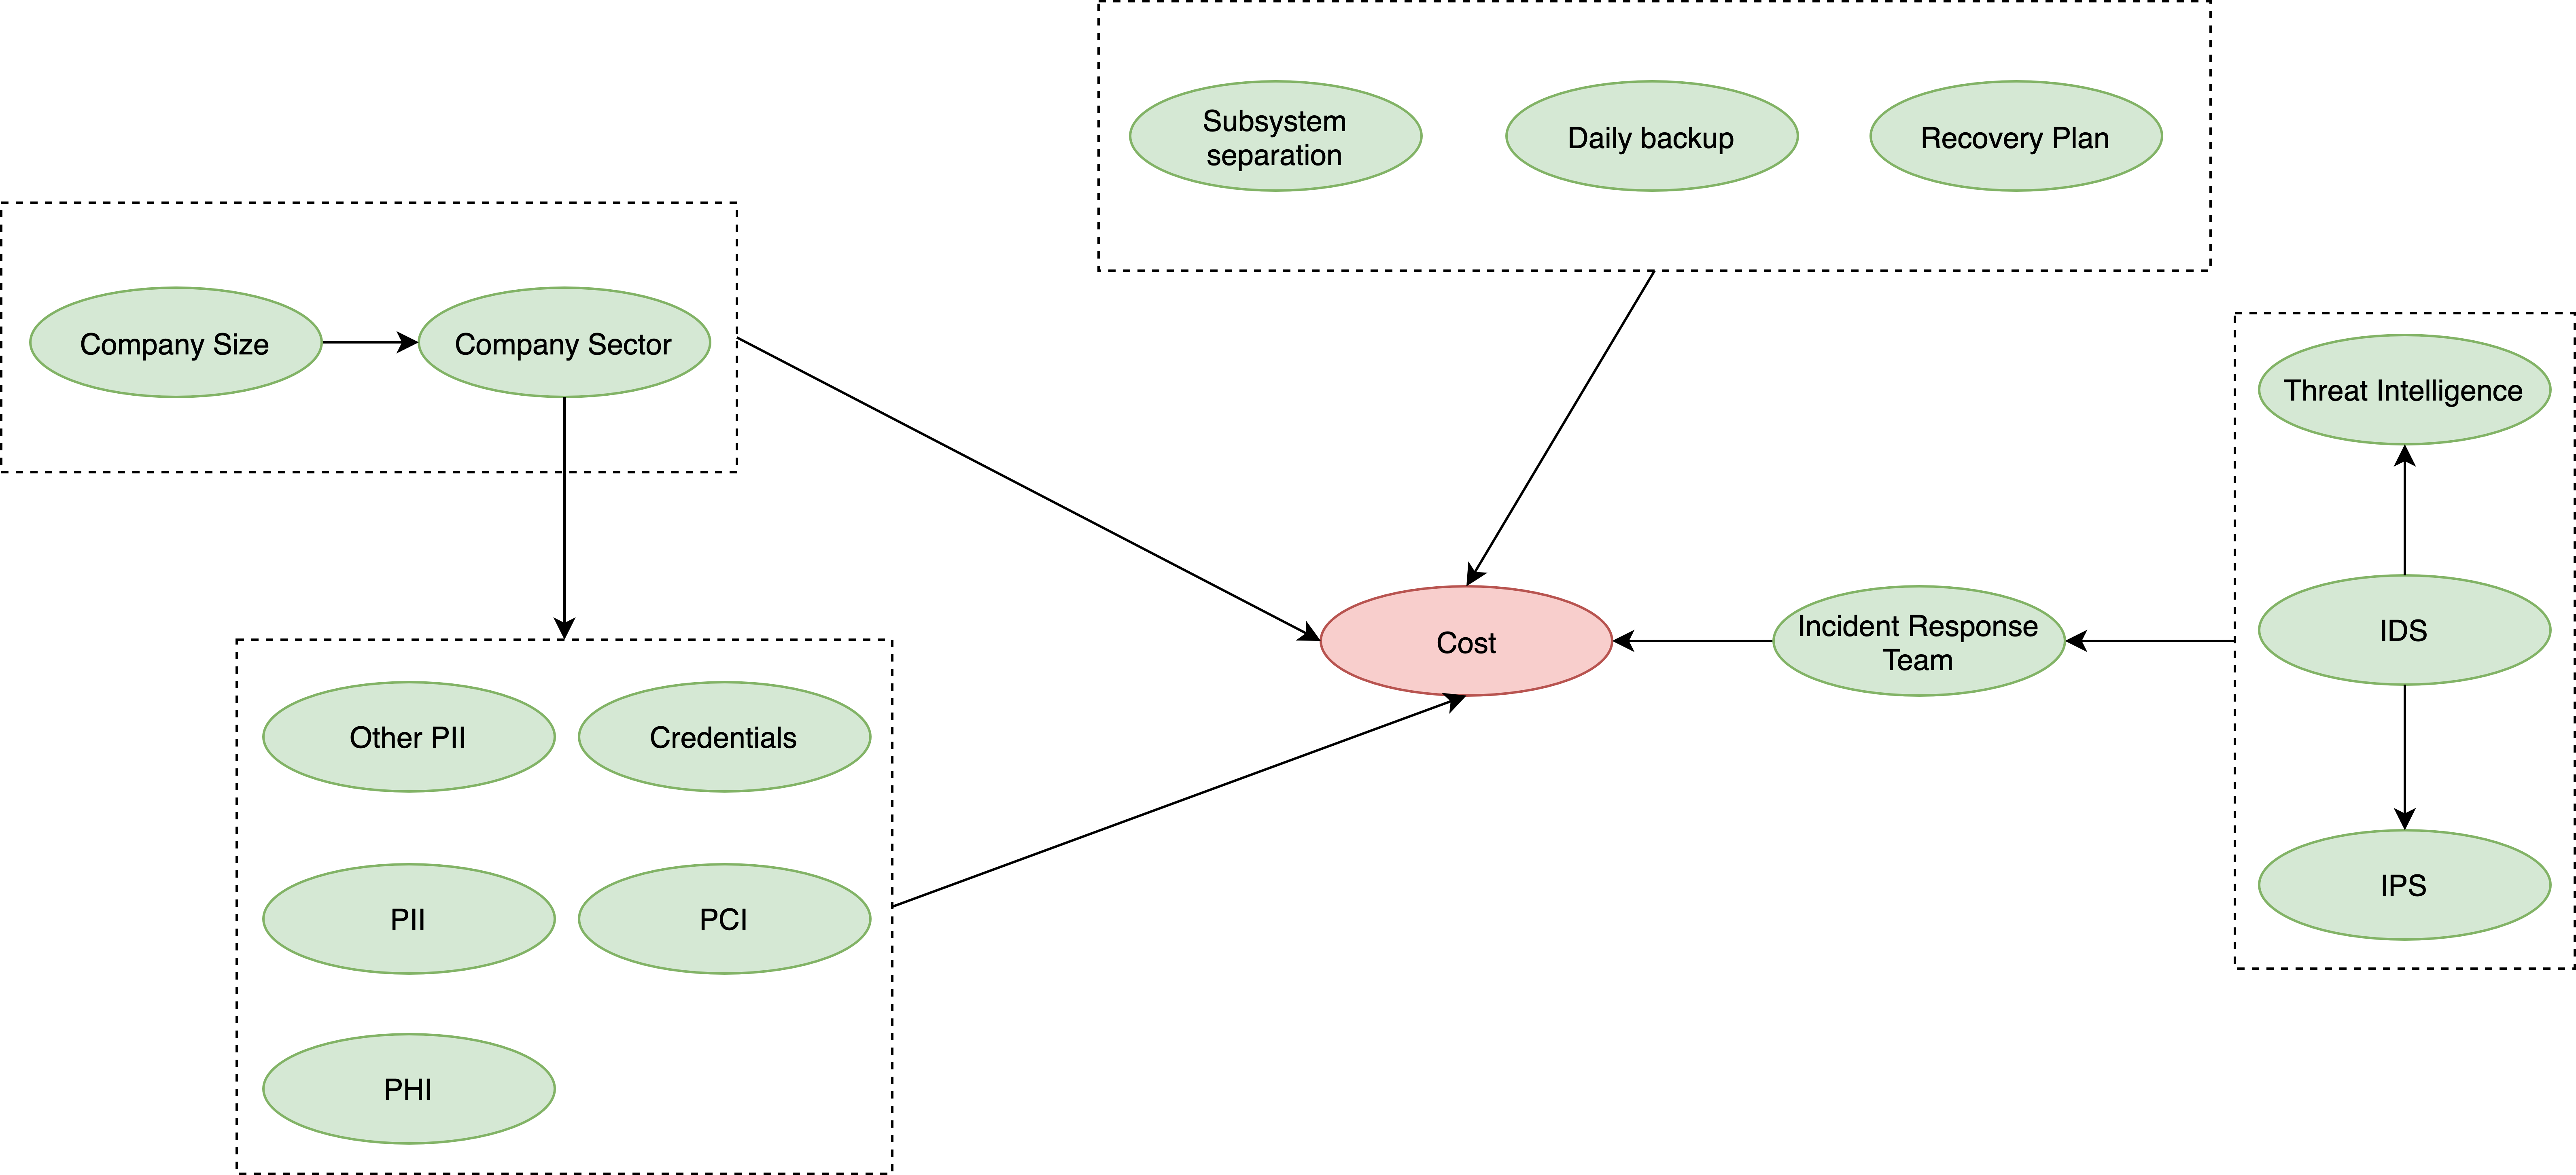
\includegraphics[scale=0.6]{images/synthetic/cost.png}
	\caption{\label{fig:cost} Features that influence the \textit{cost} target.}
\end{figure}

We generate 4 synthetic datasets, each of 1 million samples, using this new approach. The distributions of the targets are depicted in Figure ~\ref{fig:distribution-hard}.

\section{Data generation}\label{section:generation}

We start the data generation process by first creating what we called an \textit{instance stereotype}. An instance stereotype is an instance with a defined set of features (e.g. $company\_has\_antivirus: True, \; company\_has\_IDS: True, \; company\_has\_IPS: False, \; \dots$).  In practice, we expect that instances may share the same features while having slightly different target values. This is because there are many other factors that influence the \textit{loss} and \textit{cost} targets in real life, which are not captured here. For instance, two companies may both have an incident response team but their process may differ, and incident containment could take  the first company two hours and the second one two days, which may in turn impact the \textit{cost} target.  To model these differences, we rely on a log normal distribution.

\begin{definition}[Log normal distribution]
Let $Z$ be a standard normal variable, and let $\mu$ and $\sigma > 0$ be two real numbers. Then, the distribution of the random variable $X=e^{\mu+\sigma Z}$ is called the log-normal distribution with parameters $\mu$ and $\sigma$. \\

\textbf{Note}: $\mu$ and $\sigma$ are the parameters of the variable's natural logarithm, not of $X$ itself. In order to produce a distribution with desired mean $\mu_X$ and standard deviation $\sigma_X$, one uses $\mu=\ln\left(\frac{\mu_X^2}{\sqrt{\left(\mu_X^2 + \sigma_X^2\right)}}\right)$ and $\sigma = \sqrt{\ln\left(1 + \frac{\sigma_X^2}{\mu_X^2}\right)}$.
\end{definition}

We start with some instance stereotype and derive additional instances that share the same features but slightly different target values: the target values are now drawn from the log normal distribution. For example, if we have an instance stereotype with \textit{loss} probability 0.30, we model a log normal distribution with mean $\mu_X = 0.30$ and standard deviation $\sigma_{X} = 0.30 / 100 * 15$ (i.e. 15\% deviation). Instances that stem from this instance stereotype will have their \textit{loss} target drawn at random from the associated log normal distribution. Each stereotype will contribute to generating $1\%$ of the total number of samples. Algorithm ~\ref{algo:generate_data} details the procedure to generate the synthetic datasets.

\begin{algorithm}
	\DontPrintSemicolon
	\SetKwComment{Comment}{$\triangleright$\ }{}
	\SetCommentSty{itshape}
	\SetKwBlock{Begin}{function}{end function}
	\caption{Synthetic data generation}\label{algo:generate_data}
	\KwIn{$n\_samples$: number of samples to generate}
	\KwOut{$n\_samples$ synthetic data points}
	$samples \gets []$ \;
	\While{len($samples$) $<$ $n\_samples$}{
		$stereotype \gets $ \textbf{NewStereotype()} \;
		$n\_stereotype \gets \ceil{n\_samples / 100}$ \;
		$samples\_stereotype \gets $ \textbf{GenerateFromStereotype(}$stereotype, \;n\_stereotype$\textbf{)} \;
		$samples \gets samples$.\textbf{extend(}$samples\_stereotype$\textbf{)} \;
	}
	\Return{$samples[:n\_samples]$} \; \;
	\Begin(NewStereotype{(}{)}){
		$profile \gets$ \textbf{Init()} \Comment*[r]{\textcolor{blue}{Initialise attributes based on Table ~\ref{table:all_probs} and ~\ref{table:probs-data}}}
		$profile.\texttt{loss} \gets Pr(loss | A, B, C, D)$ \Comment*[r]{\textcolor{blue}{Equation ~\ref{eq6}}}
		$profile.\texttt{cost} \gets \sum_{data}{cost_{data}} + \lambda_1mean(cost_{breach}) + \lambda_2cost_{remediation}$ \Comment*[r]{\textcolor{blue}{Equation ~\ref{eq7}}}
		\Return{$profile$}
	} \;
	\Begin(GenerateFromStereotype{(}$stereotype$: \texttt{Stereotype}, $n\_stereotype$: \texttt{int}{)}){
		$samples \gets []$ \;
		$\mu_{loss}, \; \sigma_{loss} = \ln\left(\frac{stereotype.\texttt{loss}^2}{\sqrt{(stereotype.\texttt{loss}^2 + (stereotype.\texttt{loss}*0.15)^2)}}\right), \; \sqrt{\ln(1 + \frac{(stereotype.\texttt{loss}*0.15)^2}{stereotype.\texttt{loss}^2})}$ \;
		$\mu_{cost}, \; \sigma_{cost} = \ln\left(\frac{stereotype.\texttt{cost}^2}{\sqrt{(stereotype.\texttt{cost}^2 + (stereotype.\texttt{cost}*0.15)^2)}}\right), \; \sqrt{\ln(1 + \frac{(stereotype.\texttt{cost}*0.15)^2}{stereotype.\texttt{cost}^2})}$ \;
		\For{$\_ = 1$ \textbf{to} $n\_stereotype$}{
			$stereotype.\texttt{loss} \gets$ \textbf{LogNormal(}$\mu_{loss}, \; \sigma_{loss}$\textbf{)} \;
			$stereotype.\texttt{cost} \gets$ \textbf{LogNormal(}$\mu_{cost}, \; \sigma_{cost}$\textbf{)} \;
			$samples.$\textbf{append(}$stereotype$\textbf{)}
		}
		\Return{$samples$}
	}
\end{algorithm}

We evaluate the datasets through 3-fold cross-validation using our non-DP (vanilla) gradient boosting algorithm. We set the learning rate to 0.5, and the maximum depth to 15. The datasets are evaluated for [300, 5000, 15000, 25000, 50000, 75000, 100000] samples. The number of trees is fixed to 20. Figure ~\ref{fig:synthetic_data_complexity} reports the mean absolute percentage error (MAPE) obtained with the baseline model over all synthetic datasets, for both the \textit{loss} and \textit{cost} targets. Table ~\ref{table:synthetic_error_rate} reports the mean absolute percentage error rate for each dataset and target, where $n\_samples = 300$ is ignored so that the mean isn't skewed upward, as the learning task is much more difficult with this low amount of samples.

\begin{center}\begin{table}[h!]
	\center
	\noindent\makebox[0pt]{}{
		\begin{tabular}{|c|c|c|}
 		\hline
 		Dataset & Target: \textit{loss} & Target: \textit{cost} \\ [0.5ex] \hline\hline
 		Synthetic A & $3.44 \pm 0.11$ & $2.08 \pm 0.21$ \\ \hline
 		Synthetic B & $2.28 \pm 0.13$ & $1.85 \pm 0.04$ \\ \hline
 		Synthetic C & $2.22 \pm 0.12$ & $1.82 \pm 0.02$ \\ \hline
 		Synthetic D & $2.06 \pm 0.08$ & $1.85 \pm 0.04$ \\ \hline
	\end{tabular}
	\caption{\label{table:synthetic_error_rate} Mean Absolute Percentage Error (\%) for the synthetic datasets.}}
\end{table}\end{center}






\chapter{Performance Evaluation}\label{sec:evaluation}

In this chapter, we evaluate the performances of non-private GBDT and differentially private GBDT. For the latter, we compare our 2-nodes algorithm versus the classic depth-first tree induction algorithm. We use 3 real datasets not related to cyber insurance, and 4 synthetic cyber insurance datasets (since no real publicly released datasets are available). For the real datasets, we follow the literature and report the root mean square error (RMSE) for regression tasks, and the test error (in \%) for classification tasks. For the synthetic datasets, we report the mean absolute percentage error (MAPE, in \%).

\section{Datasets}

We evaluate the different models on the following datasets:

\begin{itemize}
	\item Abalone\footnote{\href{https://archive.ics.uci.edu/ml/datasets/abalone}{https://archive.ics.uci.edu/ml/datasets/abalone}}: each instance describes attributes of an abalone, such as their sex, length, or weight. The prediction task is a regression task, consisting in predicting the age of the abalone. There are 8 features and 4177 instances.
	\item YearPredictionMSD\footnote{\href{https://archive.ics.uci.edu/ml/datasets/YearPredictionMSD}{https://archive.ics.uci.edu/ml/datasets/YearPredictionMSD}}: each instance describes audio features. The prediction task in a regression task, consisting in predicting the year of release of the song. There are 90 features and 515345 instances. 
	\item Adult\footnote{\href{https://archive.ics.uci.edu/ml/datasets/adult}{https://archive.ics.uci.edu/ml/datasets/adult}}: each instance gives information about the background and education of a person. The prediction task is a classification task, consisting in predicting whether a person makes more than $50k\$$ a year or not. There are 14 features and 48842 instances.
	\item Synthetic\_\{A, B, C, D\}: synthetic datasets generated according to Algorithm ~\ref{algo:generate_data}. Each dataset contains 1 million samples, and there are 28 features per instance. The prediction task is a regression task (refer to Chapter ~\ref{chap:synthetic_data} for more details).
\end{itemize}

For each dataset, we take a sample of $n = 5000$ instances. For the real datasets, we fix the tree depth to $d_{max} = 6$, the learning rate to $\eta = 0.1$ and the number of trees to $n_{trees} = 50$. For the synthetic datasets, we fix $d_{max} = 15, \; \eta = 0.5$ and $n_{trees} = 20$. The models are evaluated through a 5-cross validation process. We report results for the vanilla GBDT (non-private, as in Algorithm ~\ref{algo:gbdt}) and the differentially private GBDT algorithms (depth-first and 2-nodes variants, as in Algorithm ~\ref{algo:dp_gbdt} and ~\ref{algo:2_nodes_dpgbdt} respectively).

\newpage

\section{Results}

We use values of $\epsilon$ in the $[0.1, \ 1.[$ range. Intuitively, the higher the privacy budget $\epsilon$ is, the less noise will be added to the model. This results in better accuracy, but in lower privacy guarantees. We choose not to evaluate the model on higher privacy budgets, as the existing literature (e.g. \cite{dpgbdt}) reports great accuracy in such settings already. 

Table ~\ref{table:training_time} shows the mean training time (in seconds) per tree and per dataset. The depth-first variant implements the algorithm outlined in \cite{dpgbdt}, while the 2-nodes variant tries to enhance it. For the Abalone and YearPredictionMSD datasets, we report the root mean square error (RMSE) for our model. For the Adult dataset, we report the test error (in \%). 

\begin{center}\begin{table}[h!]
	\center
	\noindent\makebox[0pt]{}{
		\begin{tabular}{|c|c|c|c|}
 		\hline
 		 & (Non-DP) Vanilla & (DP) Depth-first & (DP) 2-nodes \\ [0.5ex] \hline\hline
 		Abalone & 2.44 & 0.26 & 0.33 \\ \hline
 		YearPredictionMSD & 85.3 & 11.92 & 12.06 \\ \hline
 		Adult & 0.87 & 0.17 & 0.16 \\ \hline
 		Synthetic A & 0.37 & 0.40 & 0.42 \\ \hline
 		Synthetic B & 0.30 & 0.41 & 0.41 \\ \hline
 		Synthetic C & 0.68 & 0.41 & 0.41 \\ \hline
 		Synthetic D & 0.27 & 0.40 & 0.40 \\ \hline
	\end{tabular}
	\caption{\label{table:training_time} Mean training time (in seconds) per decision tree, for all datasets.}}
\end{table}\end{center}

\begin{figure}[h!]
  \begin{subfigure}{\linewidth}
  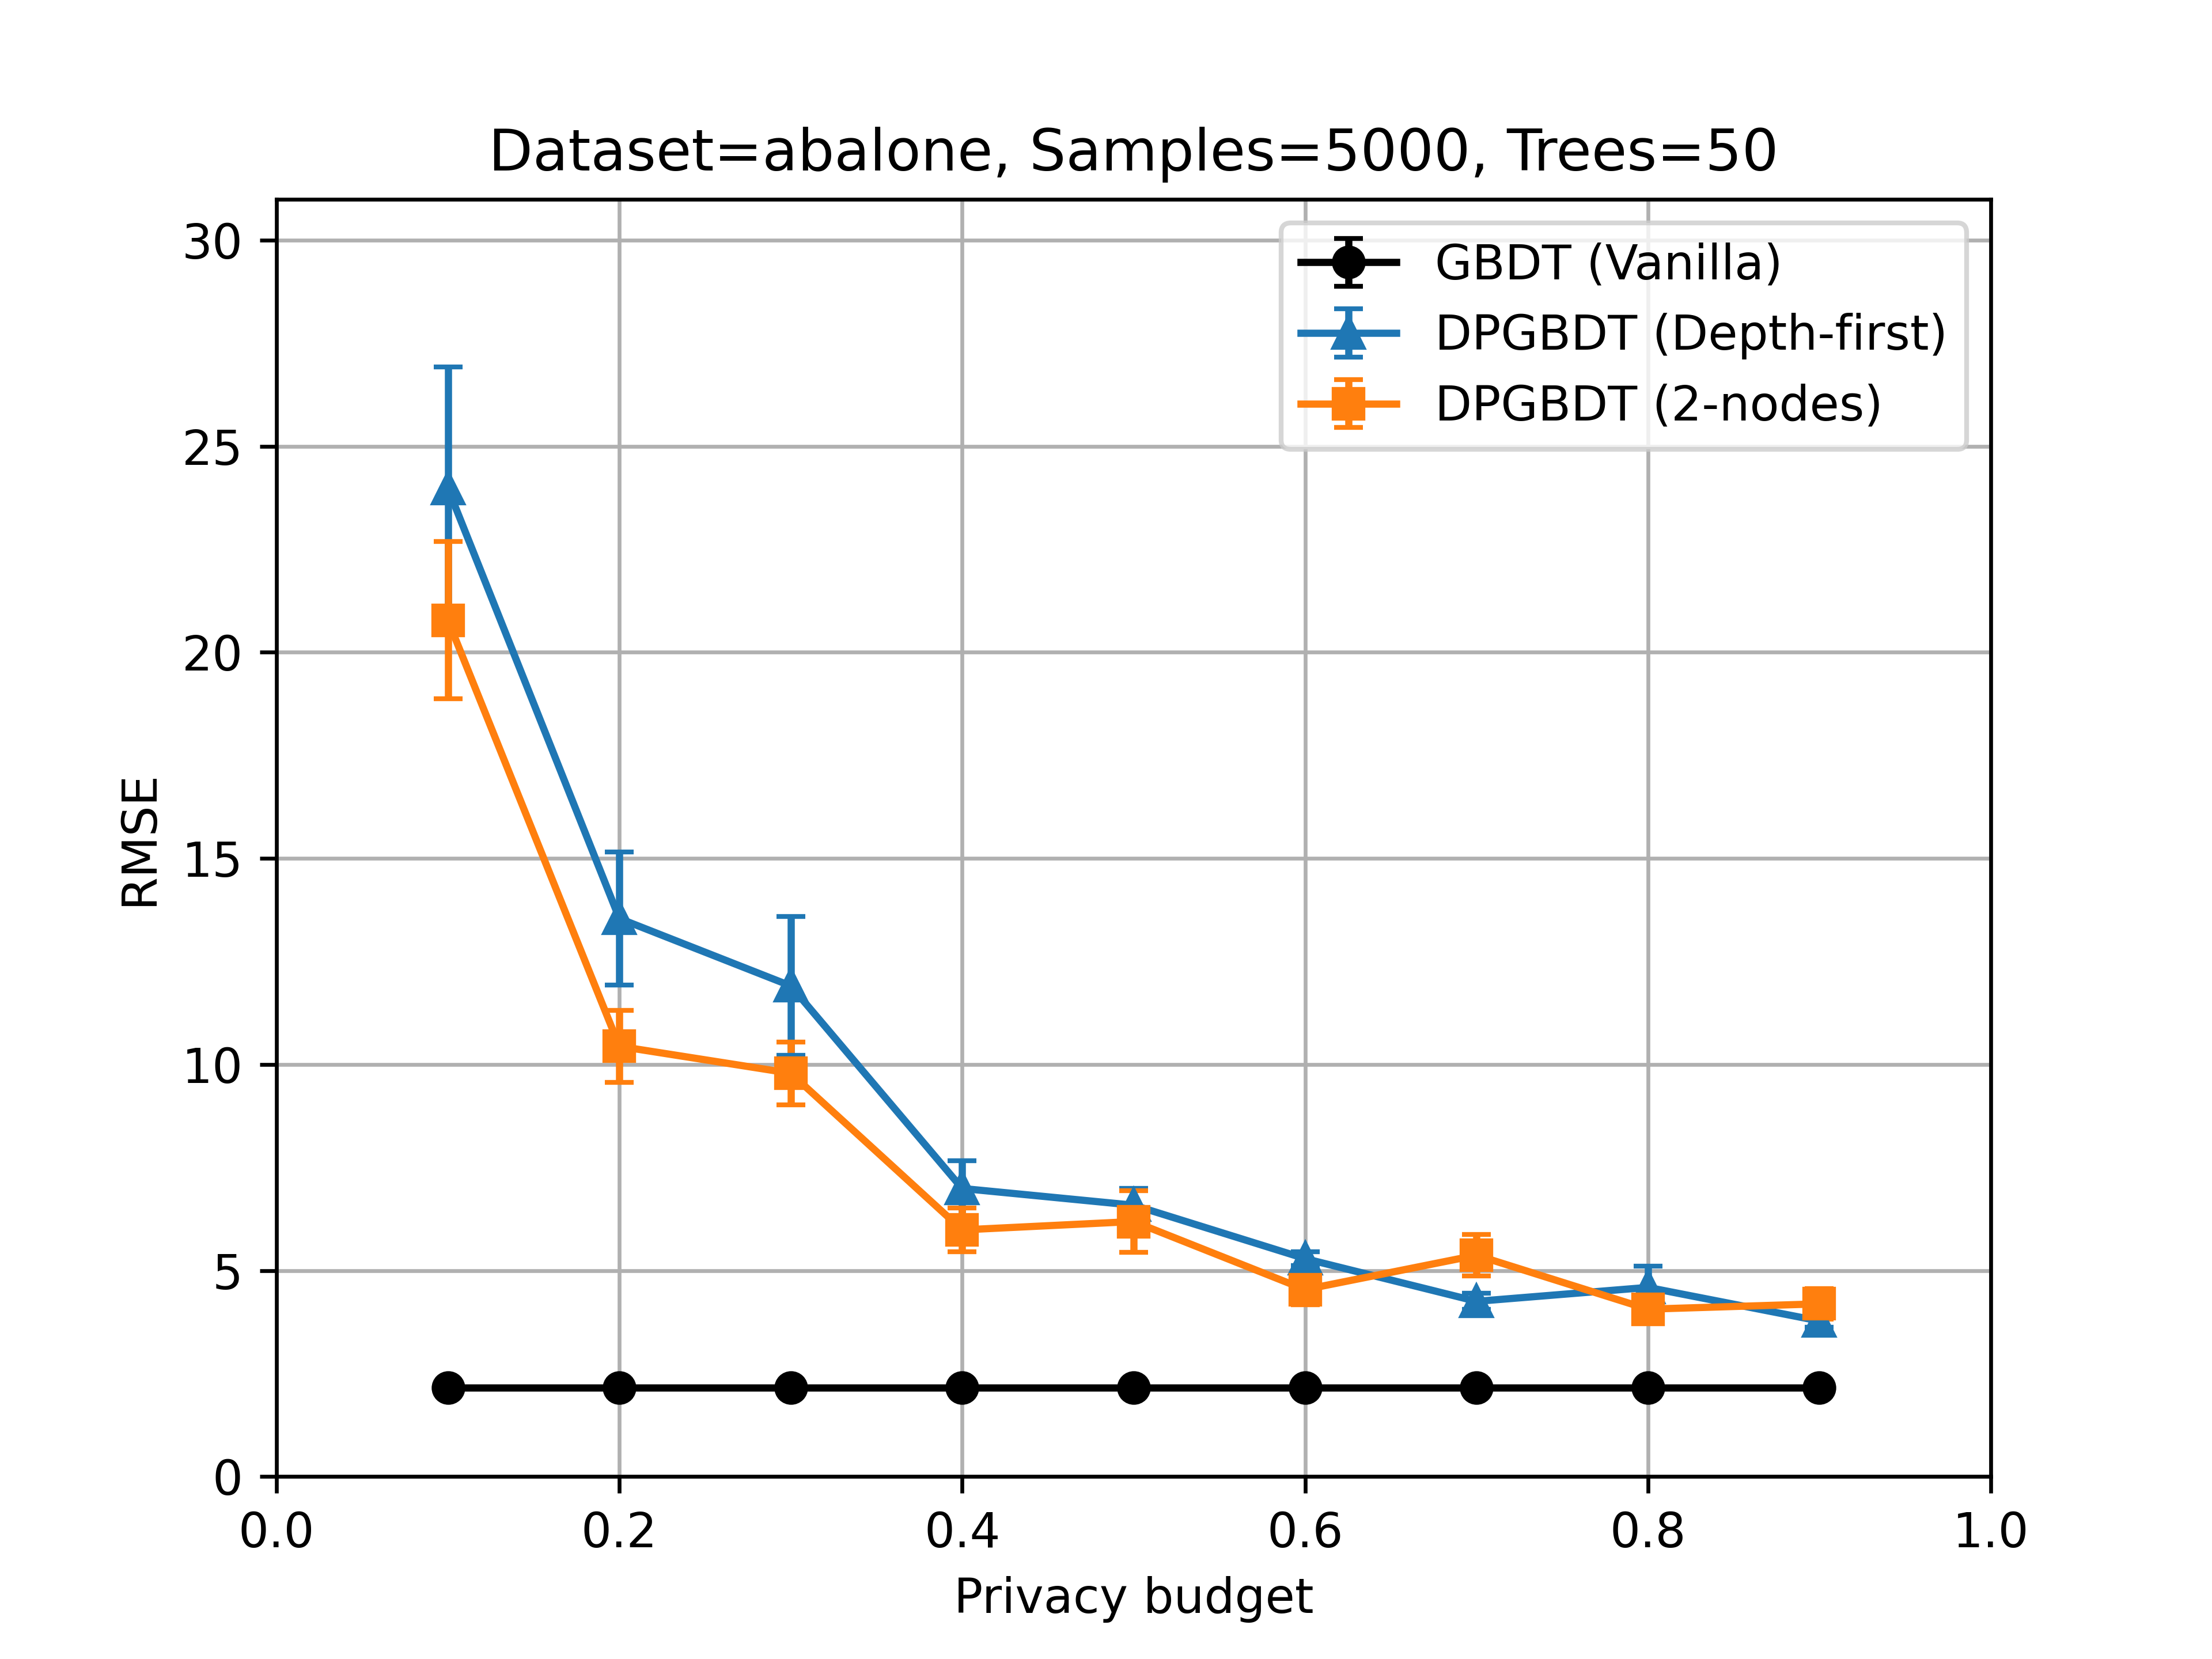
\includegraphics[width=.5\linewidth]{images/evaluation/abalone_5000.png}\hfill
  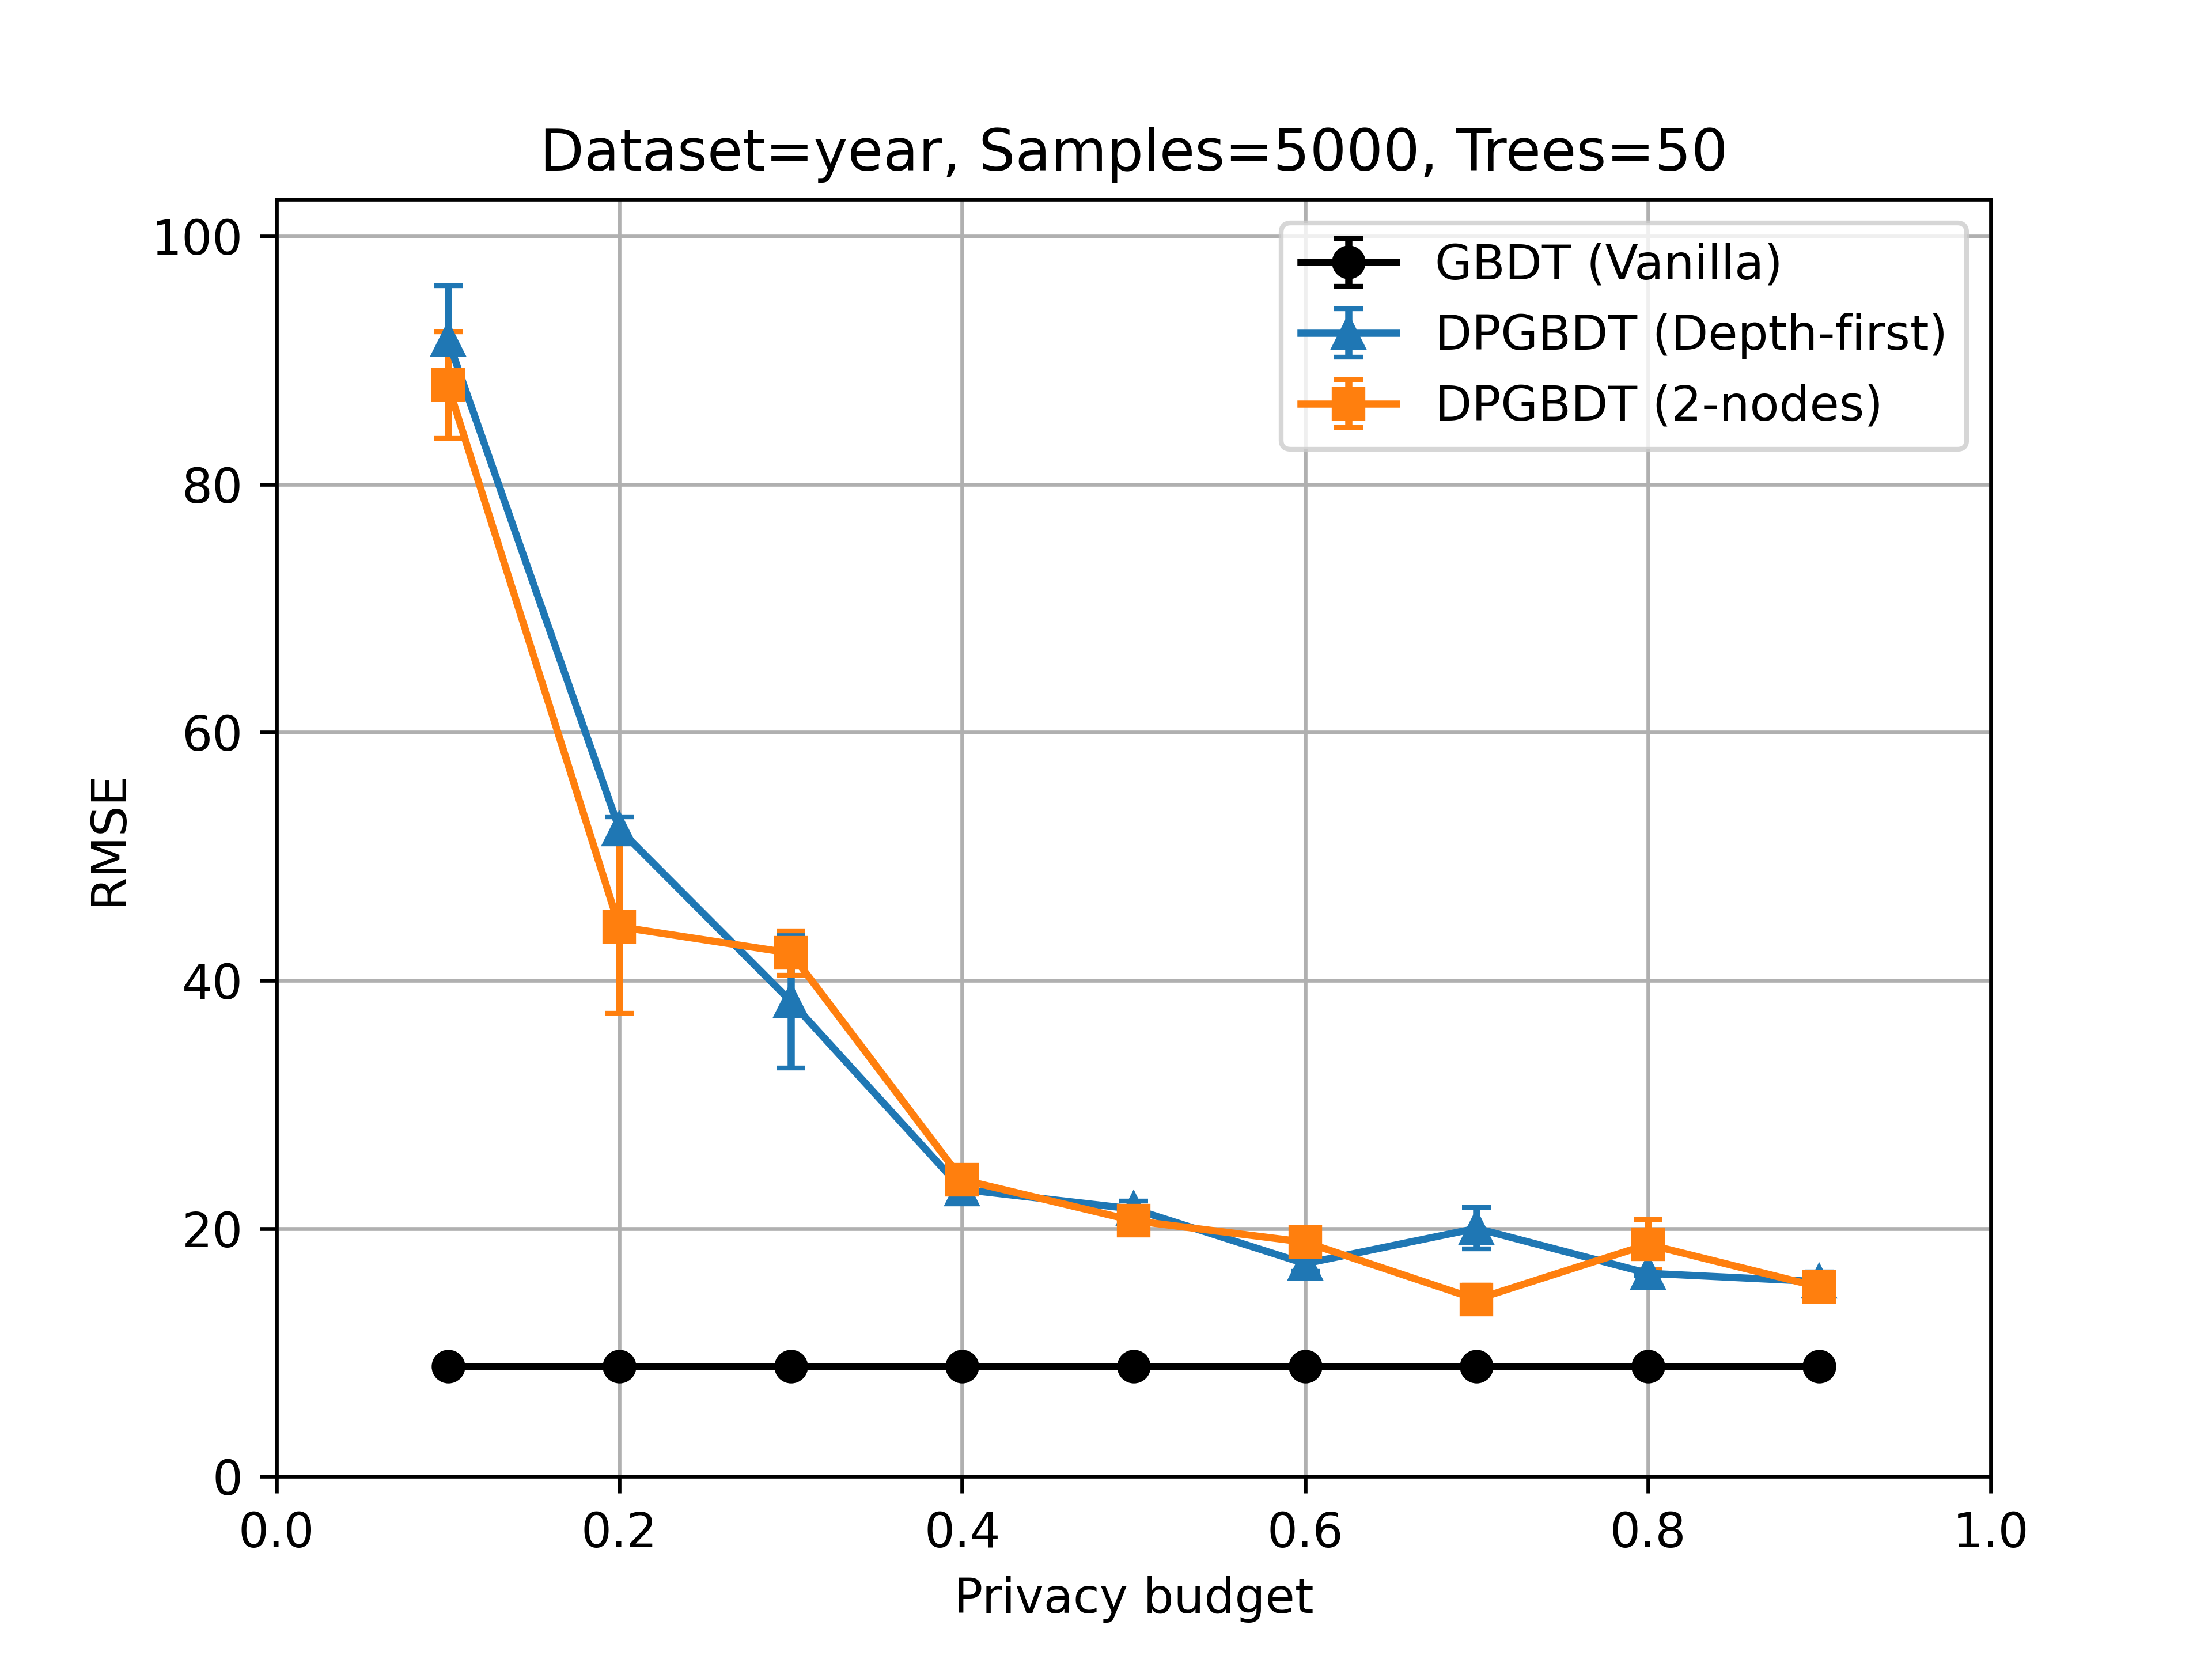
\includegraphics[width=.5\linewidth]{images/evaluation/year_5000.png}
  \caption{Regression tasks: Abalone and YearPredictionMSD}
  \end{subfigure}\par\medskip
  \begin{subfigure}{\linewidth}
  \center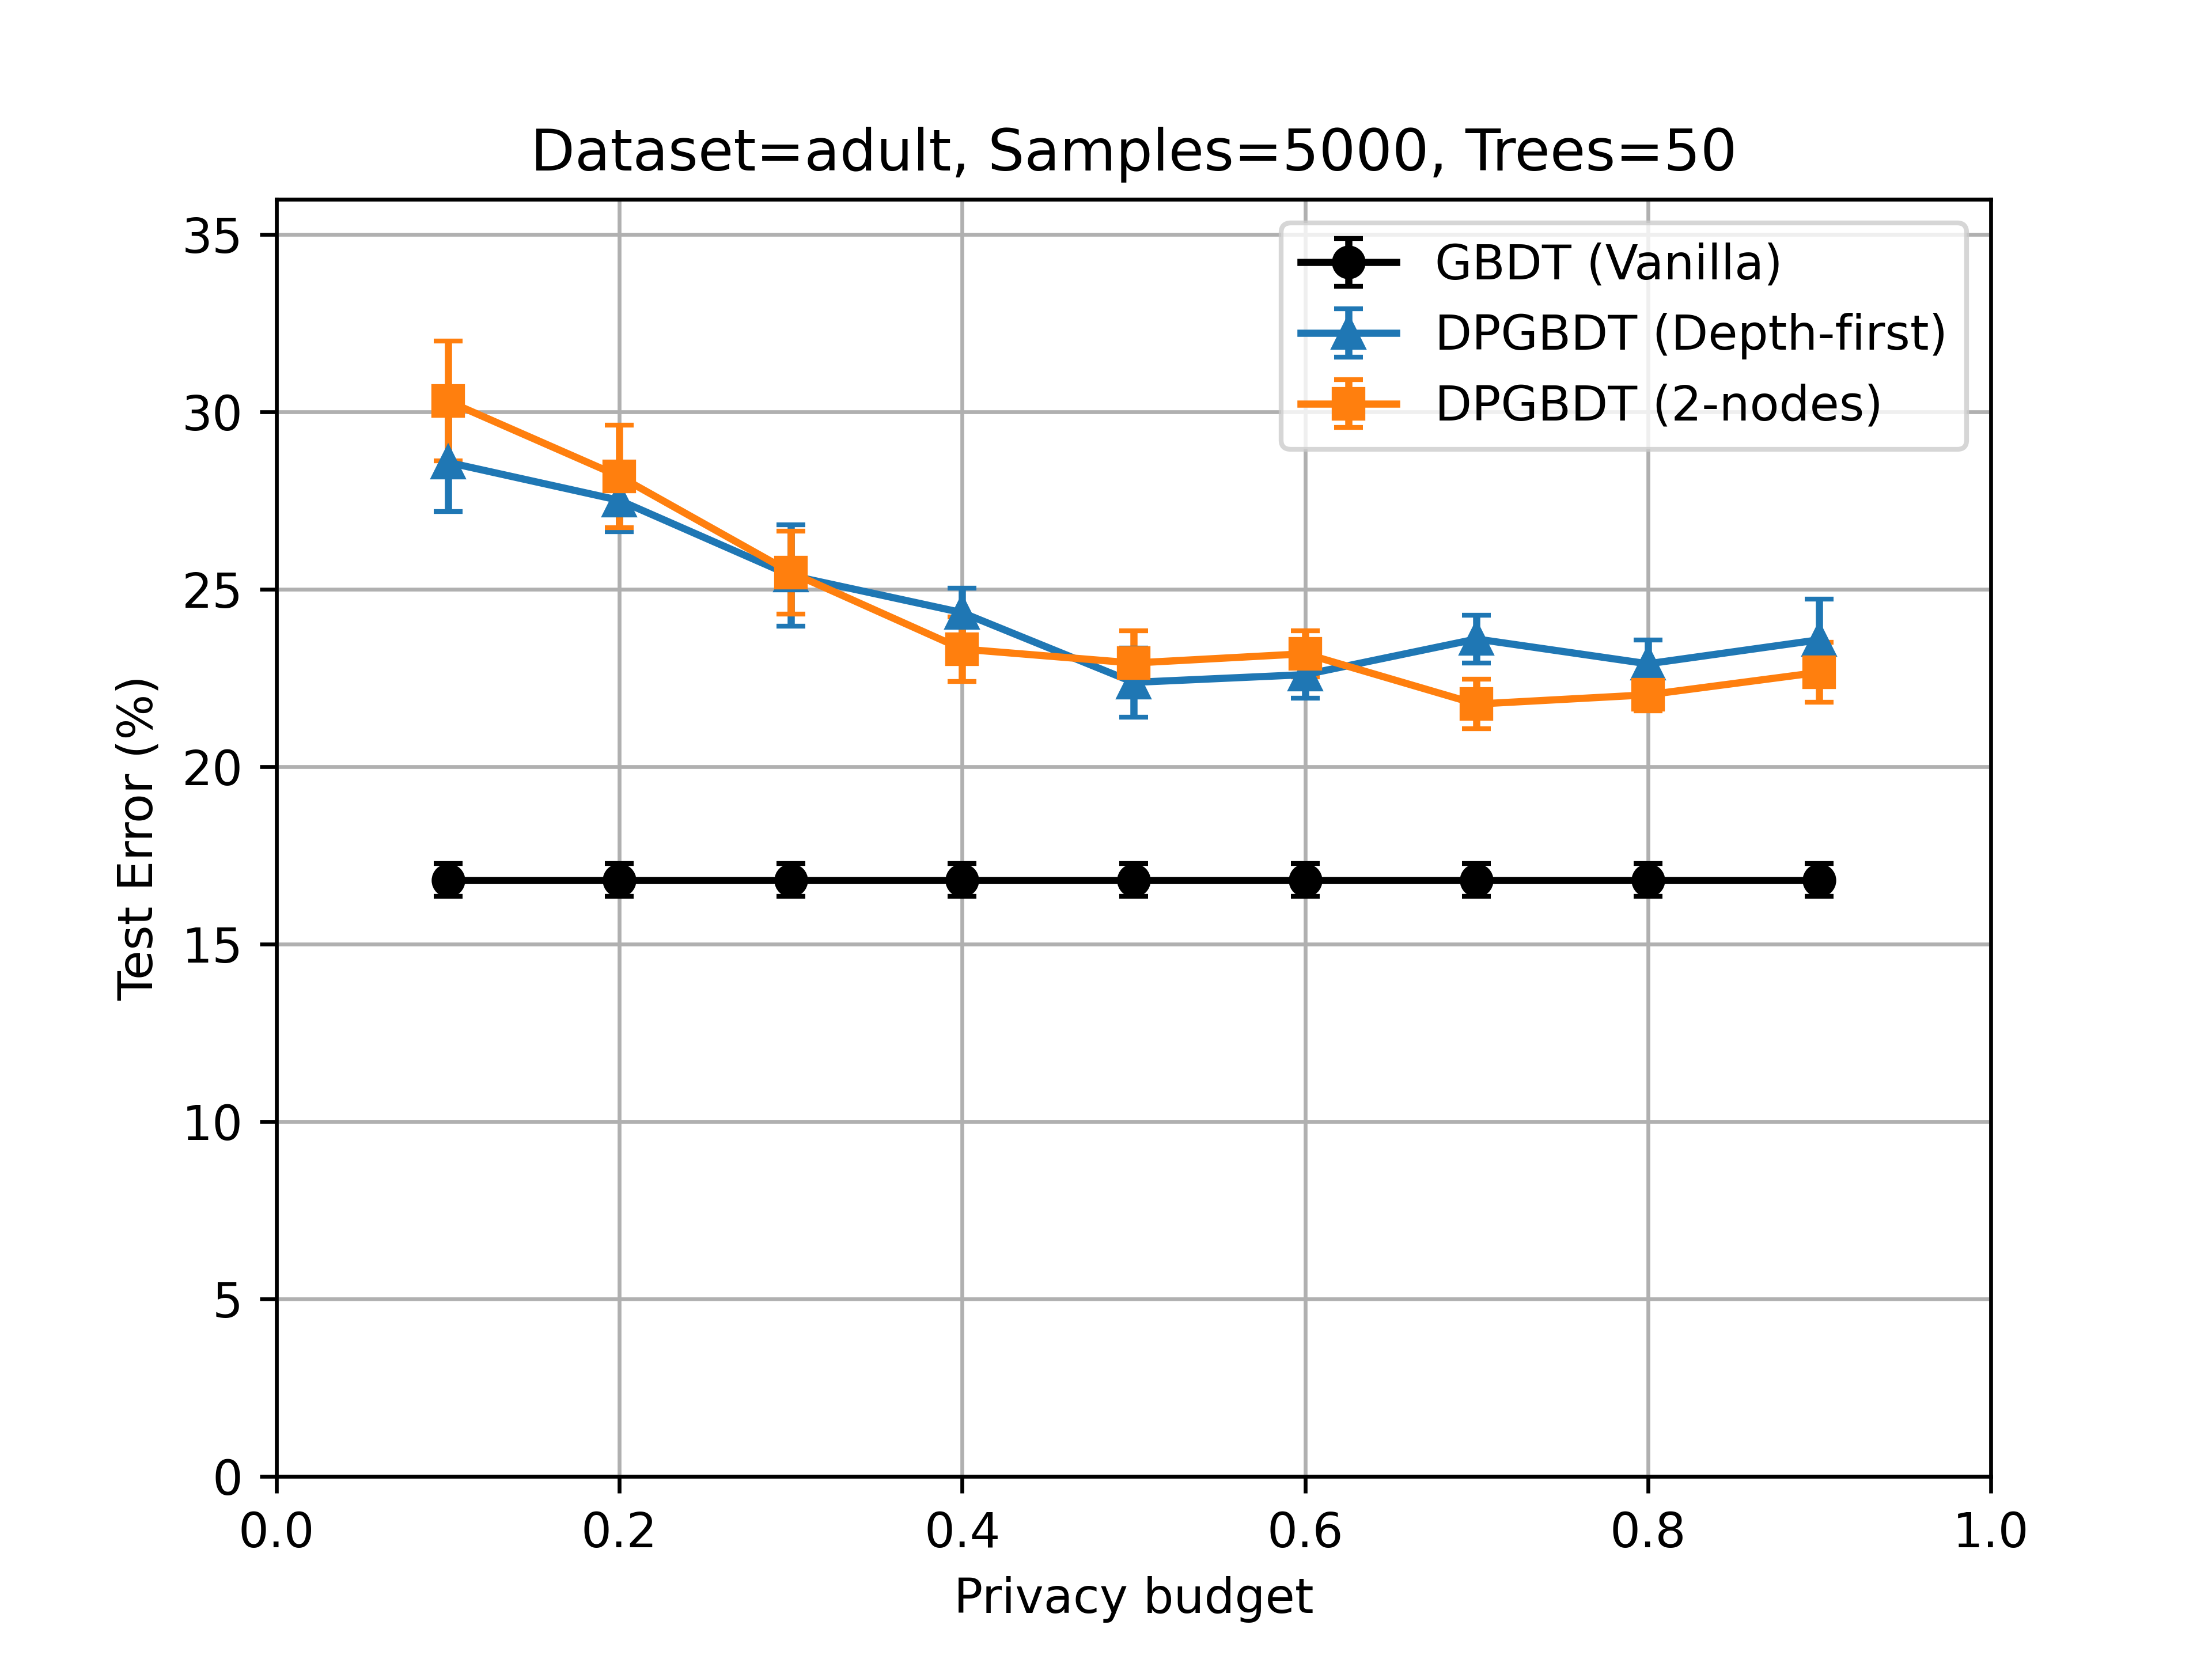
\includegraphics[width=.5\linewidth]{images/evaluation/adult_5000.png}
  \caption{Classification task: Adult}
  \end{subfigure}
  \caption{\label{fig:results_real}Prediction error for the vanilla model and various values of $\epsilon$ for the differentially private model.}
\end{figure}

\begin{figure}[h!]
	\center
	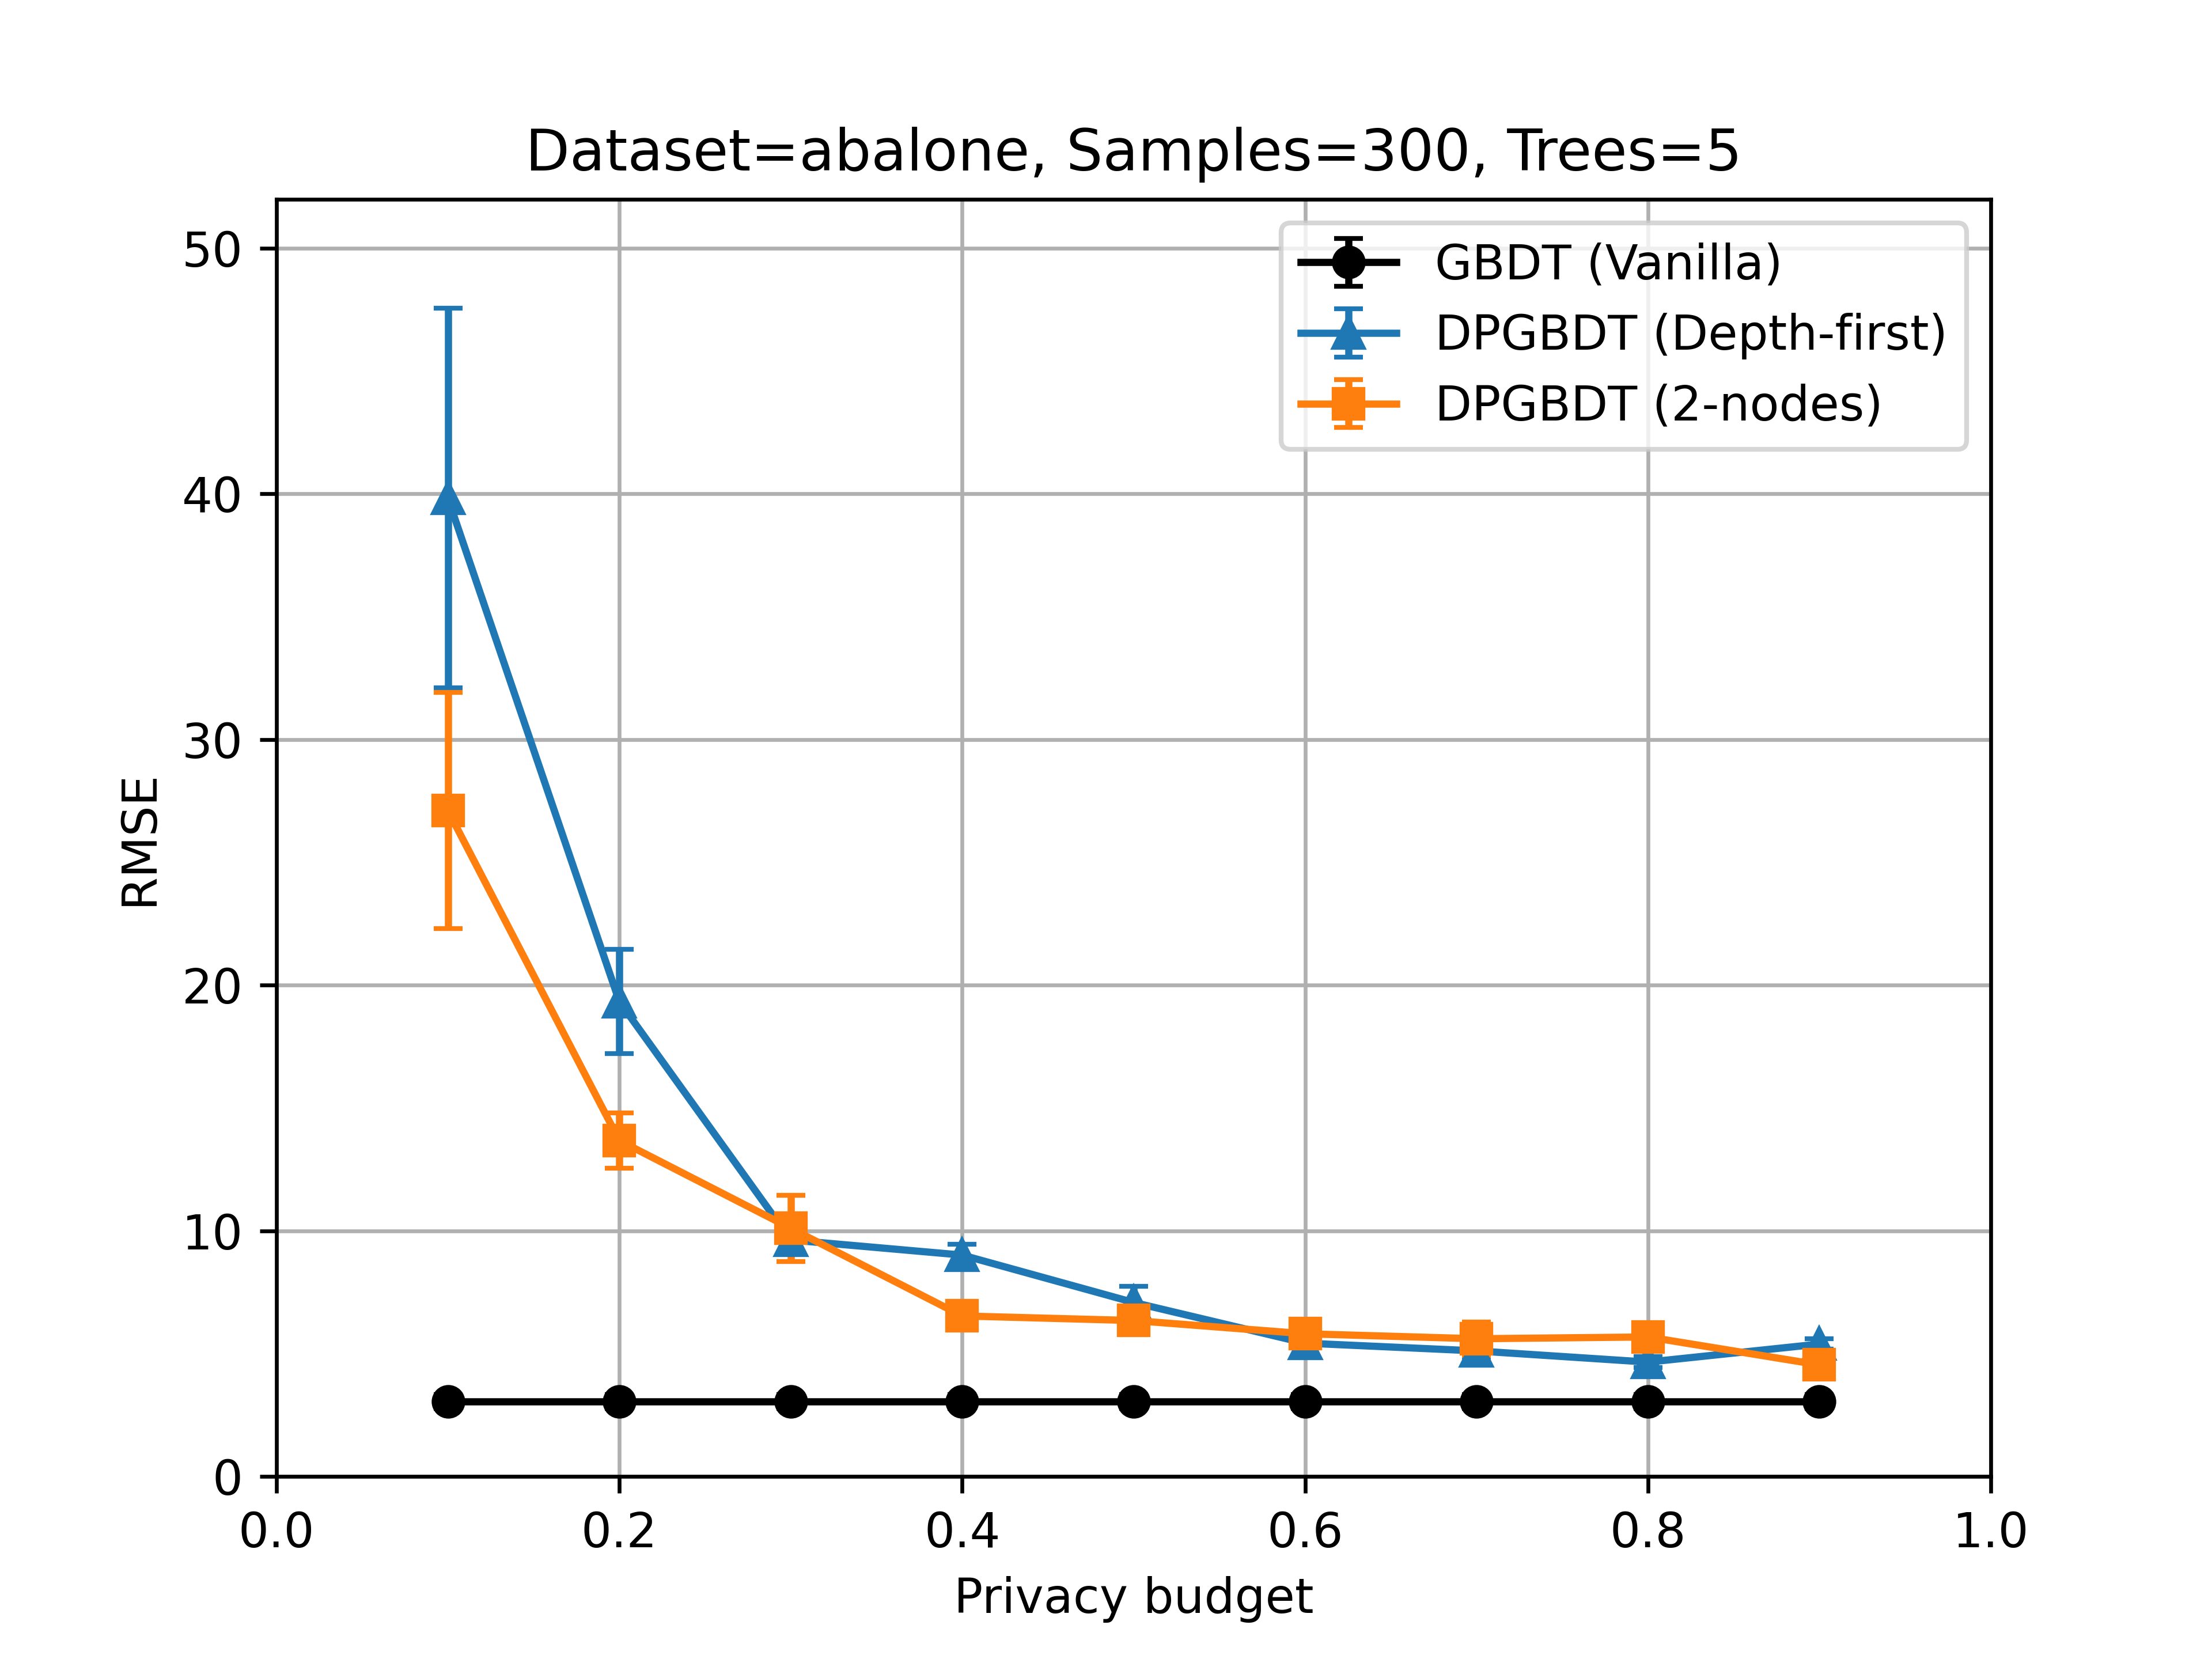
\includegraphics[width=.5\linewidth]{images/evaluation/abalone_300.png}
	\caption{\label{fig:abalone_300} Prediction error for the Abalone dataset, with 300 samples.}
\end{figure}

As shown in Figure ~\ref{fig:results_real}, our 2-nodes induction method performs slightly better than the regular depth-first induction method. This is especially visible in the Abalone dataset when $\epsilon$ is low and when we decrease the number of samples to $n = 300$ and the number of trees to $n_{trees} = 5$, where for $\epsilon=0.1$ our \textit{2-nodes} model performs $31.94\%$ better than the regular depth-first model. (reported in Figure ~\ref{fig:abalone_300}).

Table ~\ref{table:pred_results_real} summarises the results for the vanilla model versus the differentially private model (where the privacy budget is fixed to $\epsilon = 0.5$) on these real-life datasets.

\begin{center}\begin{table}[h!]
	\center
	\noindent\makebox[0pt]{}{
		\begin{tabular}{|c|c|c|c|}
 		\hline
 		 & (Non-DP) Vanilla & (DP) Depth-first & (DP) 2-nodes \\ [0.5ex] \hline\hline
 		Abalone (RMSE) & $2.15 \pm 0.04$ & $6.58 \pm 0.40$  & $\textbf{6.18} \pm \textbf{0.75}$ \\ \hline
 		YearPredictionMSD (RMSE) & $8.87 \pm 0.16$ & $21.57 \pm 0.64$ & $\textbf{20.62} \pm \textbf{0.13}$ \\ \hline
 		Adult (Test error) & $16.81 \pm 0.45$ & $\textbf{22.37} \pm \textbf{0.97}$ & $22.92 \pm 0.91$ \\ \hline
	\end{tabular}
	\caption{\label{table:pred_results_real} Prediction error for the real datasets.}}
\end{table}\end{center}

\newpage

For the synthetic datasets, we report the MAPE, defined as $MAPE = \frac{1}{n}\sum_{i}^n \abs{\frac{R_i - P_i}{R_i}}$ where $R_i$ is the real value and $P_i$ the predicted one. If the prediction task was to predict the price of an object, with its real price being $100\$$ and the predicted price being $110\$$, then the MAPE score would be $MAPE = \abs{\frac{100-110}{100}} = 0.1$ i.e. $10\%$ error, since we would be $10\$$ off. 

Results for the \textit{cost} target are reported in Figure ~\ref{fig:results_synthetic_cost}. For the \textit{loss} target, the reader can refer to Figure ~\ref{fig:results_synthetic_loss}. Table ~\ref{table:pred_results_synthetic_cost} summarises the results for the vanilla model versus the differentially private model (where the privacy budget is fixed to $\epsilon = 0.5$), for the \textit{cost} target. For the \textit{loss} target, the reader can refer to Table ~\ref{table:pred_results_synthetic_loss}.

\begin{center}\begin{table}[h!]
	\center
	\noindent\makebox[0pt]{}{
		\begin{tabular}{|c|c|c|c|}
 		\hline
 		 & (Non-DP) Vanilla & (DP) Depth-first & (DP) 2-nodes \\ [0.5ex] \hline\hline
 		Synthetic A (MAPE) & $2.90 \pm 0.80$ & $11.83 \pm 3.31$  & $\textbf{7.12} \pm \textbf{0.89}$ \\ \hline
 		Synthetic B (MAPE) & $2.69 \pm 0.79$ & $8.43 \pm 1.62$  & $\textbf{7.99} \pm \textbf{1.58}$ \\ \hline
 		Synthetic C (MAPE) & $2.13 \pm 0.36$ & $\textbf{6.88} \pm \textbf{0.71}$  & $8.52 \pm 1.74$ \\ \hline
 		Synthetic D (MAPE) & $2.05 \pm 0.16$ & $7.00 \pm 0.76$  & $\textbf{5.47} \pm \textbf{0.42}$ \\ \hline
	\end{tabular}
	\caption{\label{table:pred_results_synthetic_cost} Prediction error for the \textit{cost} target on the synthetic datasets.}}
\end{table}\end{center}

For the synthetic dataset A, 2-nodes is able to decrease the error by almost $40\%$. For datasets B and D, the error decreases by $5.22\%$ and $27.97\%$ respectively. On dataset C, 2-nodes performs worst with an error increase of $23.84\%$.

%\newpage

\begin{figure}[h!]
  \begin{subfigure}{\linewidth}
  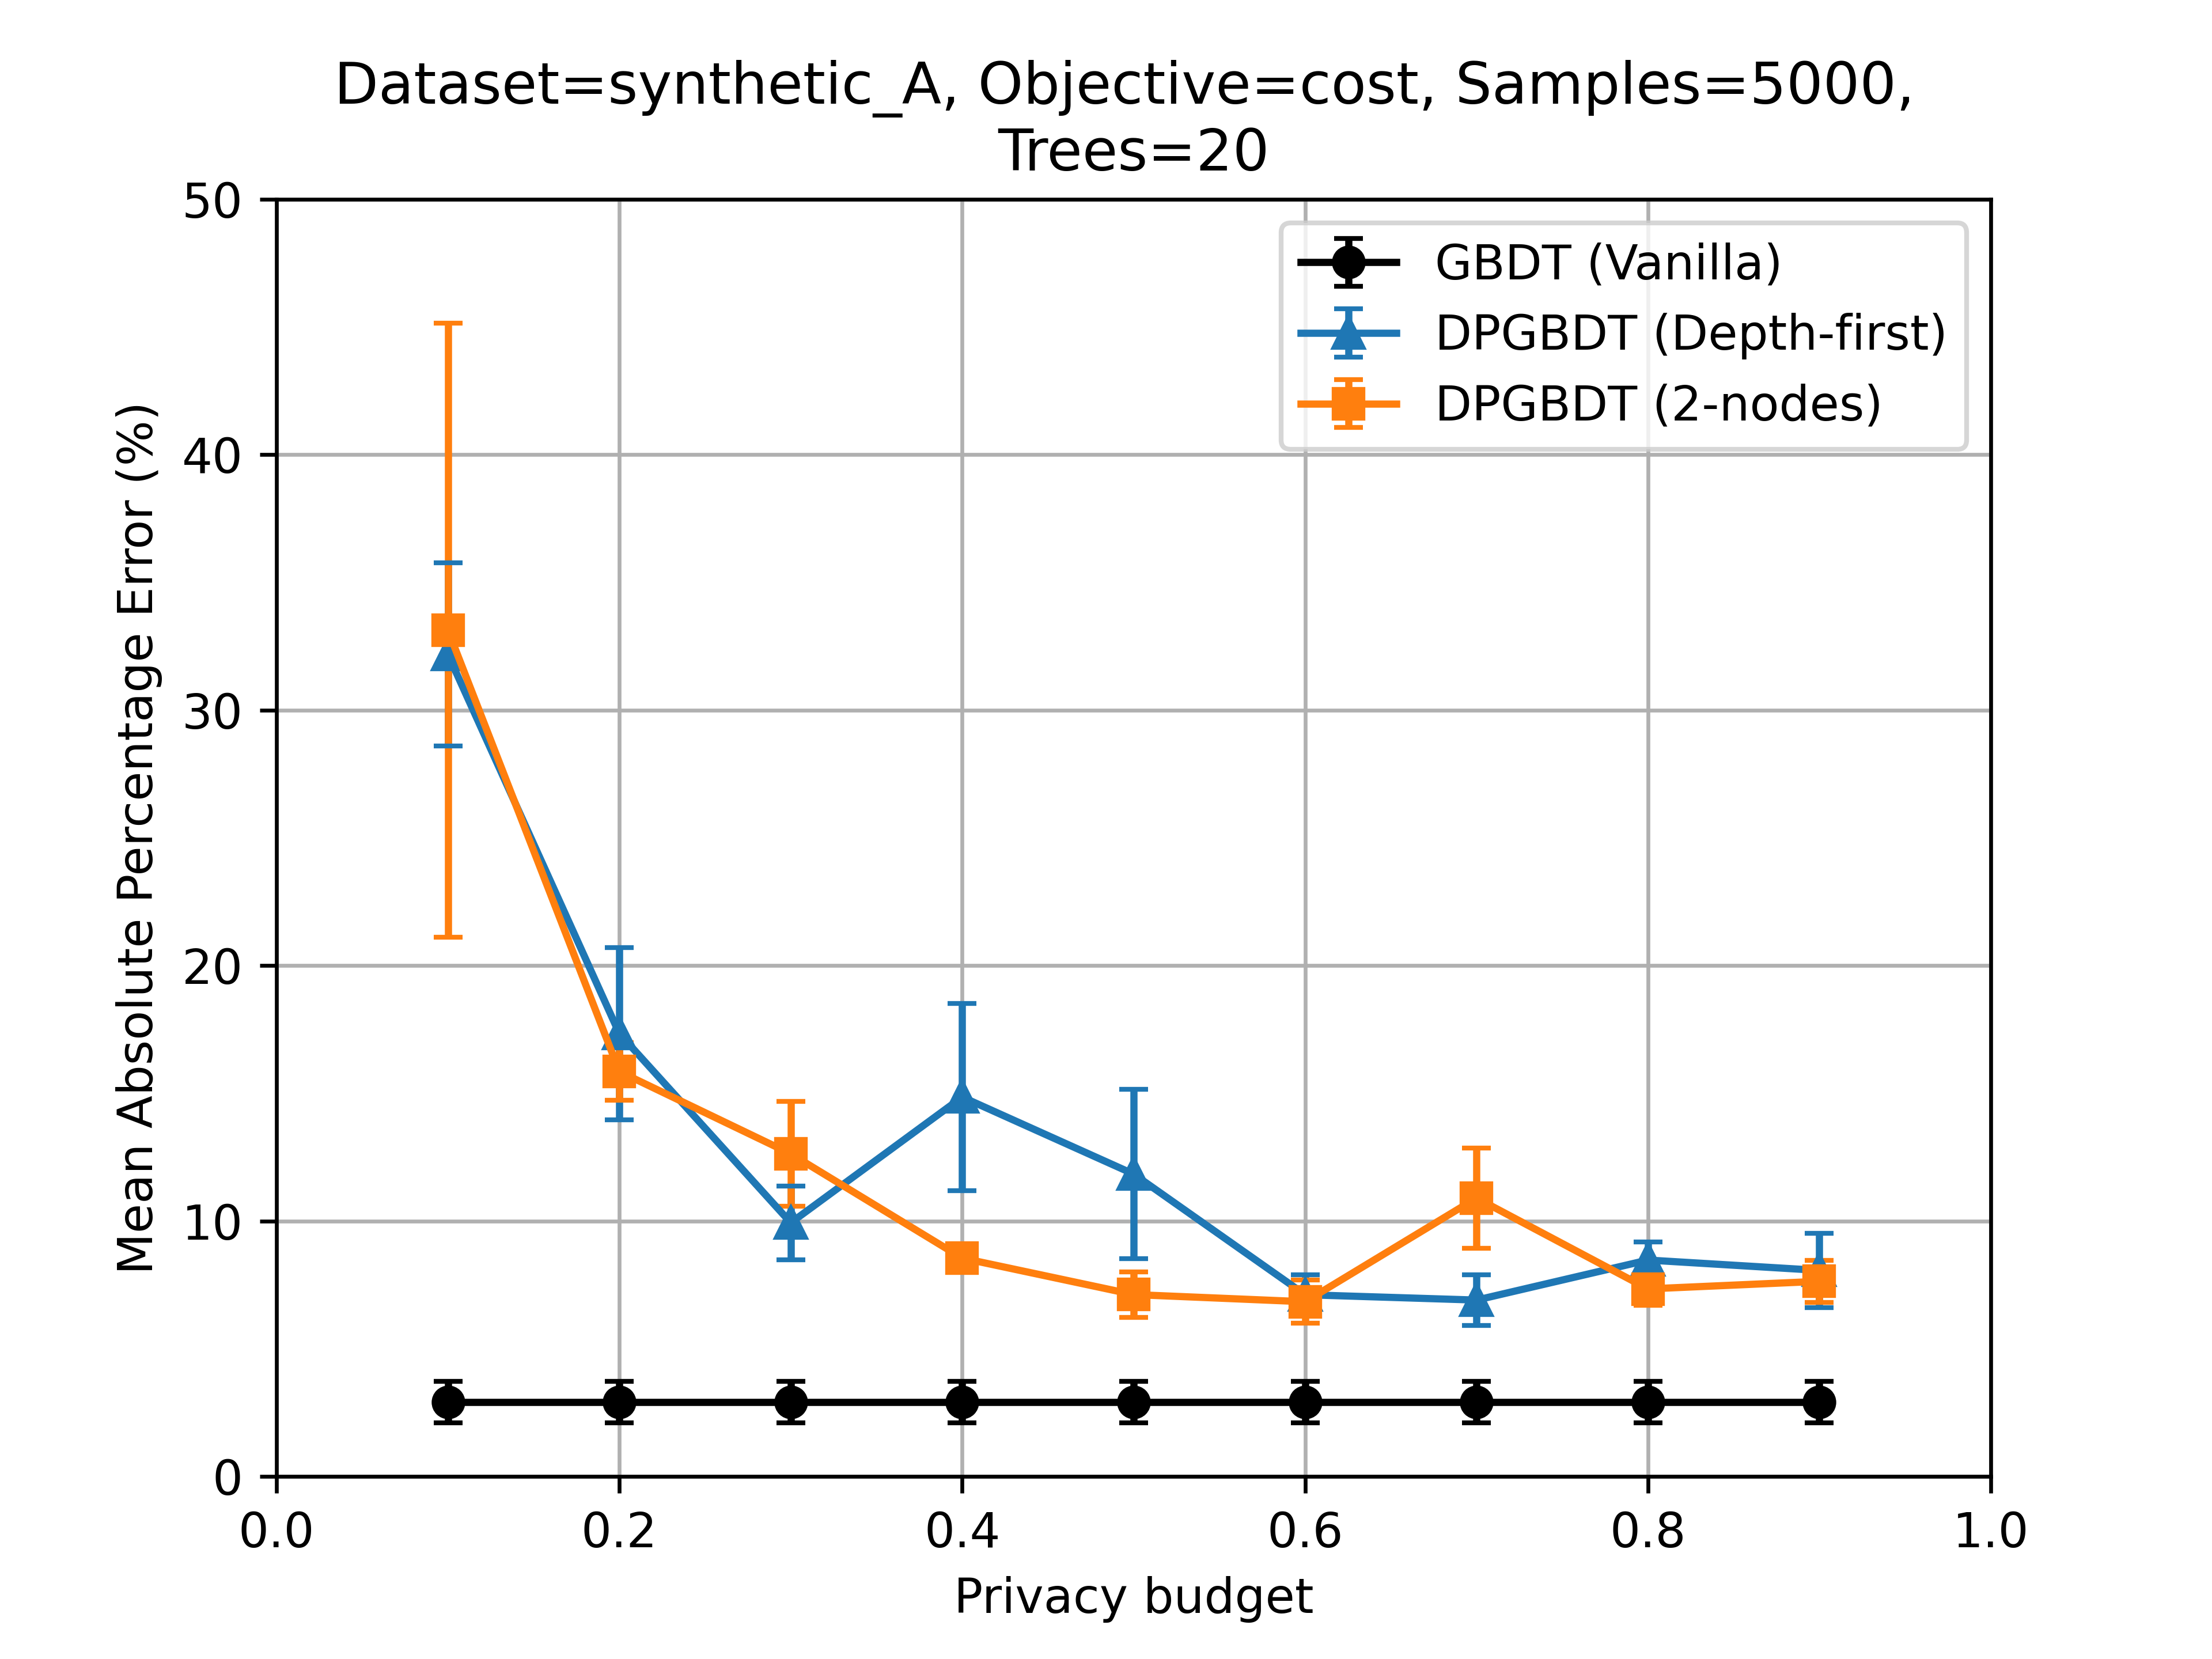
\includegraphics[width=.5\linewidth]{images/evaluation/synthetic_A_cost_5000.png}\hfill
  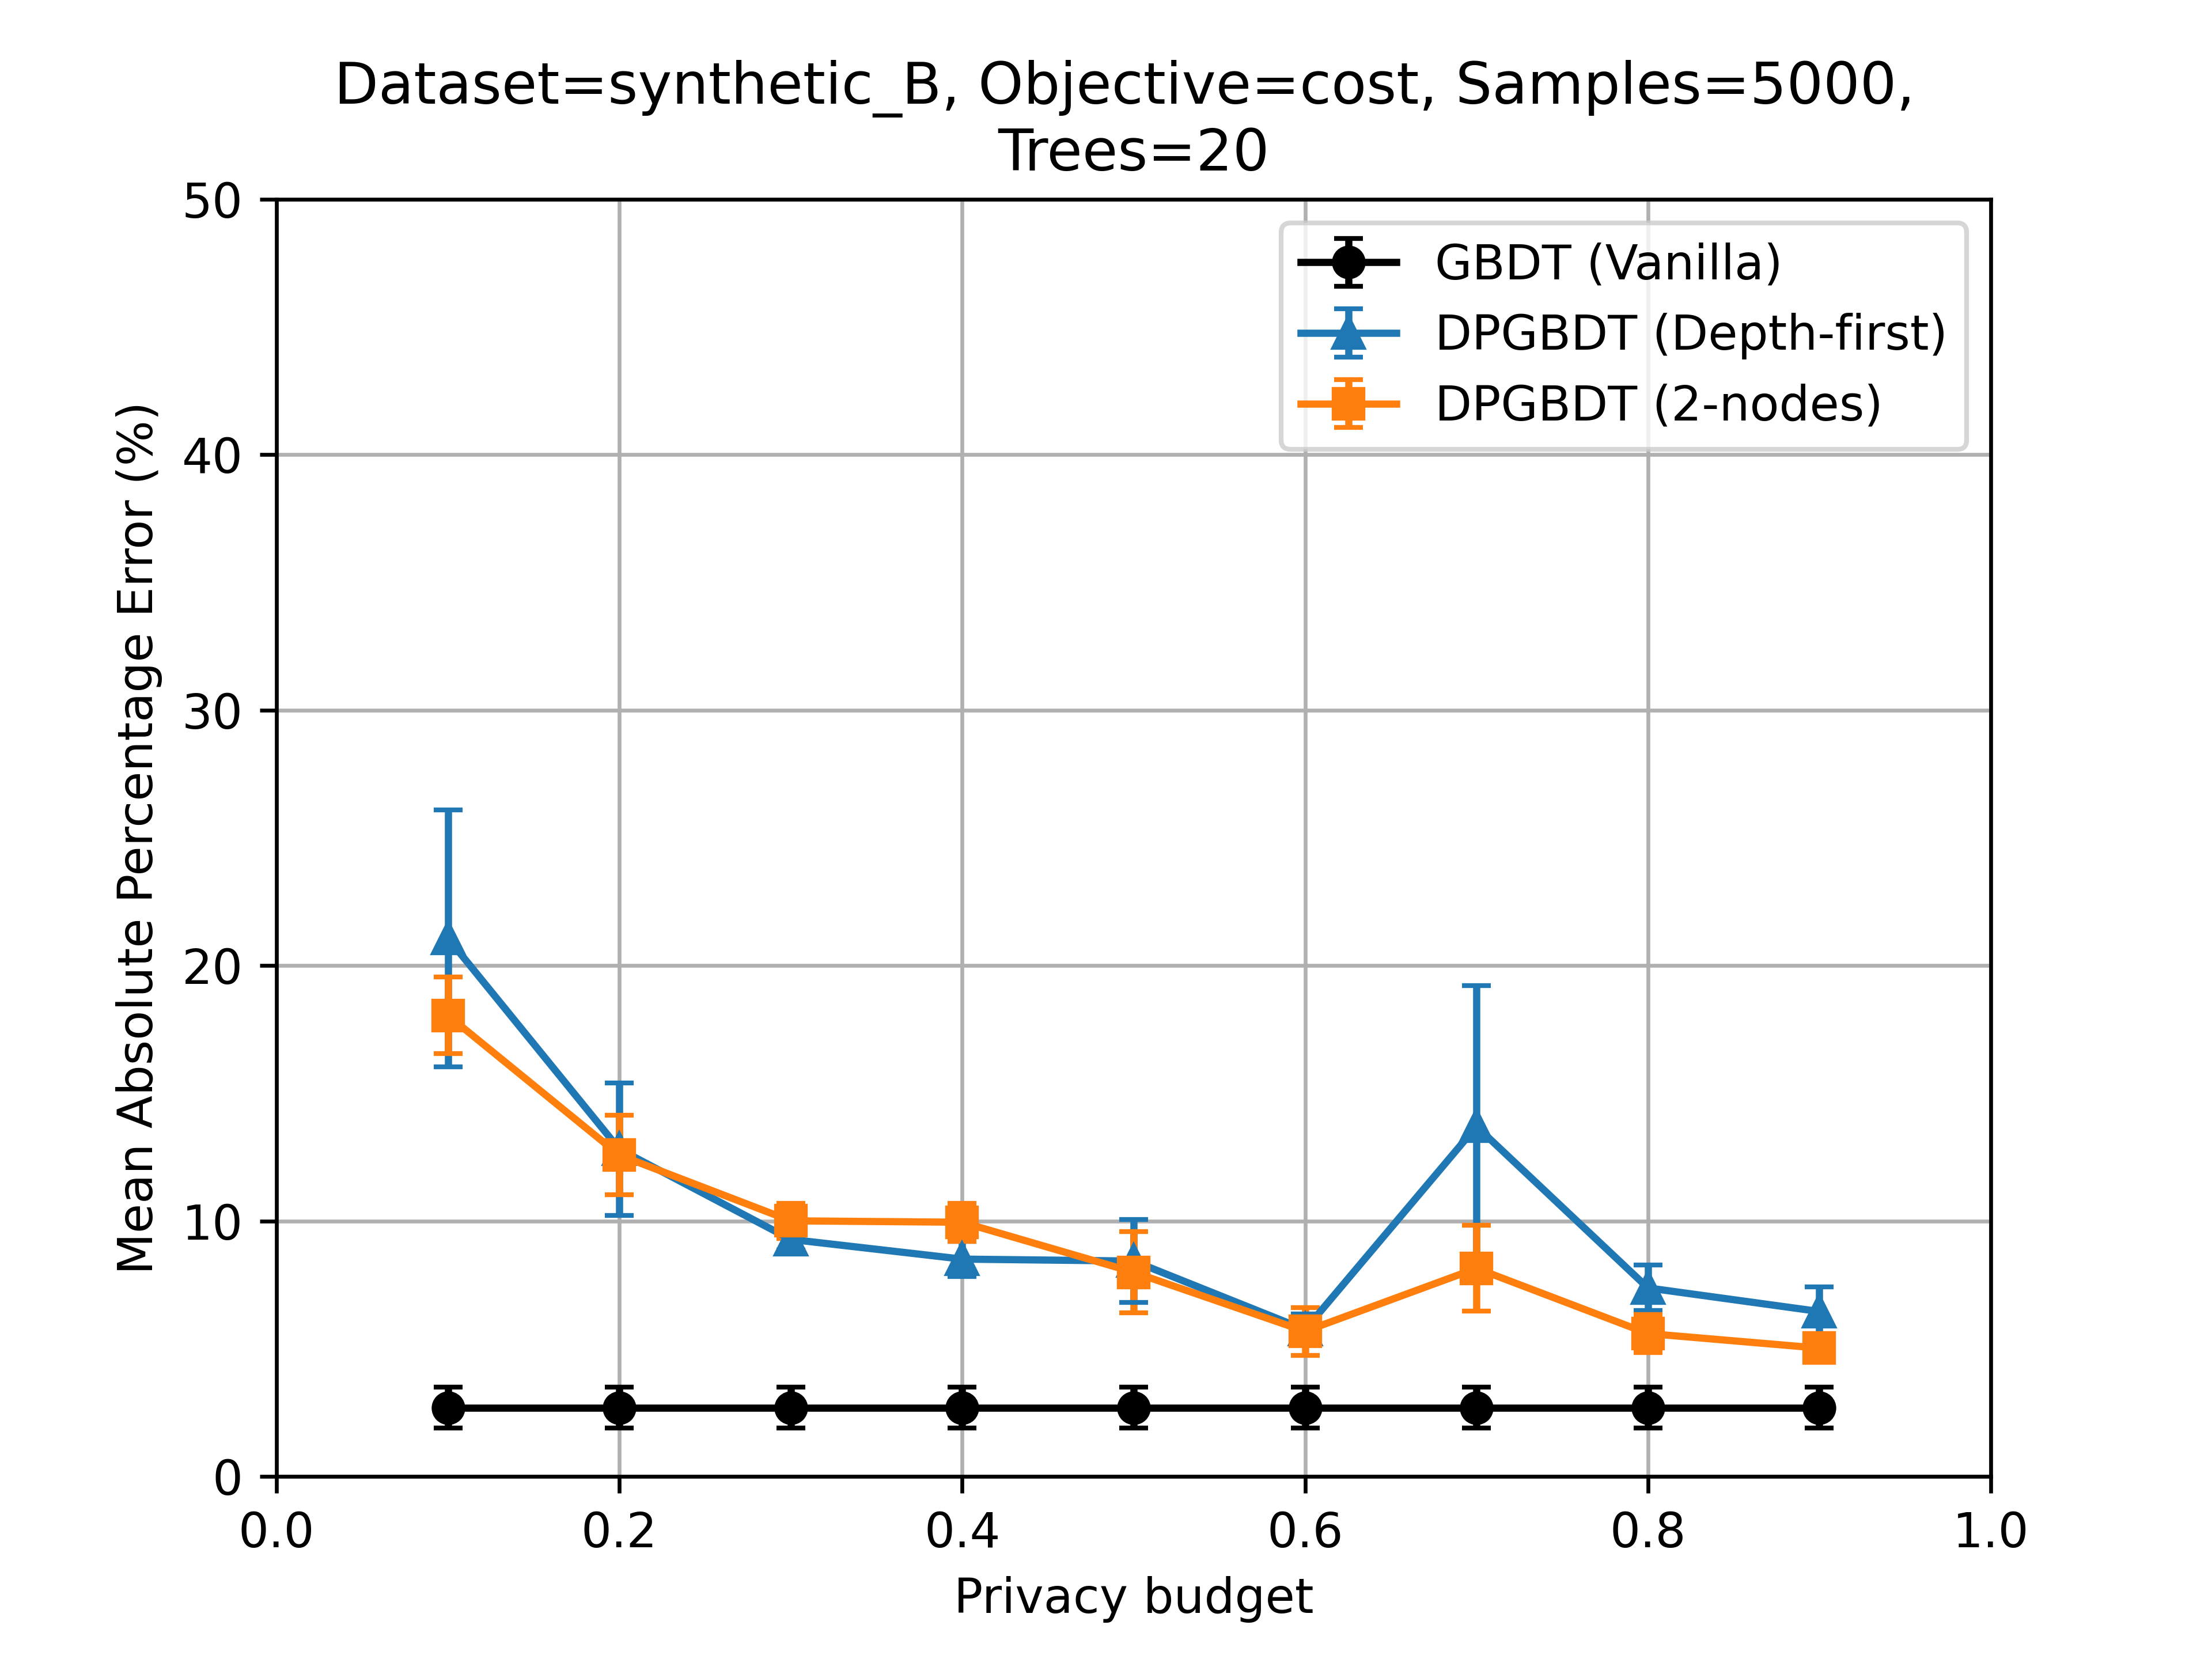
\includegraphics[width=.5\linewidth]{images/evaluation/synthetic_B_cost_5000.png}
  \caption{Synthetic datasets A and B}
  \end{subfigure}\par\medskip
  \begin{subfigure}{\linewidth}
  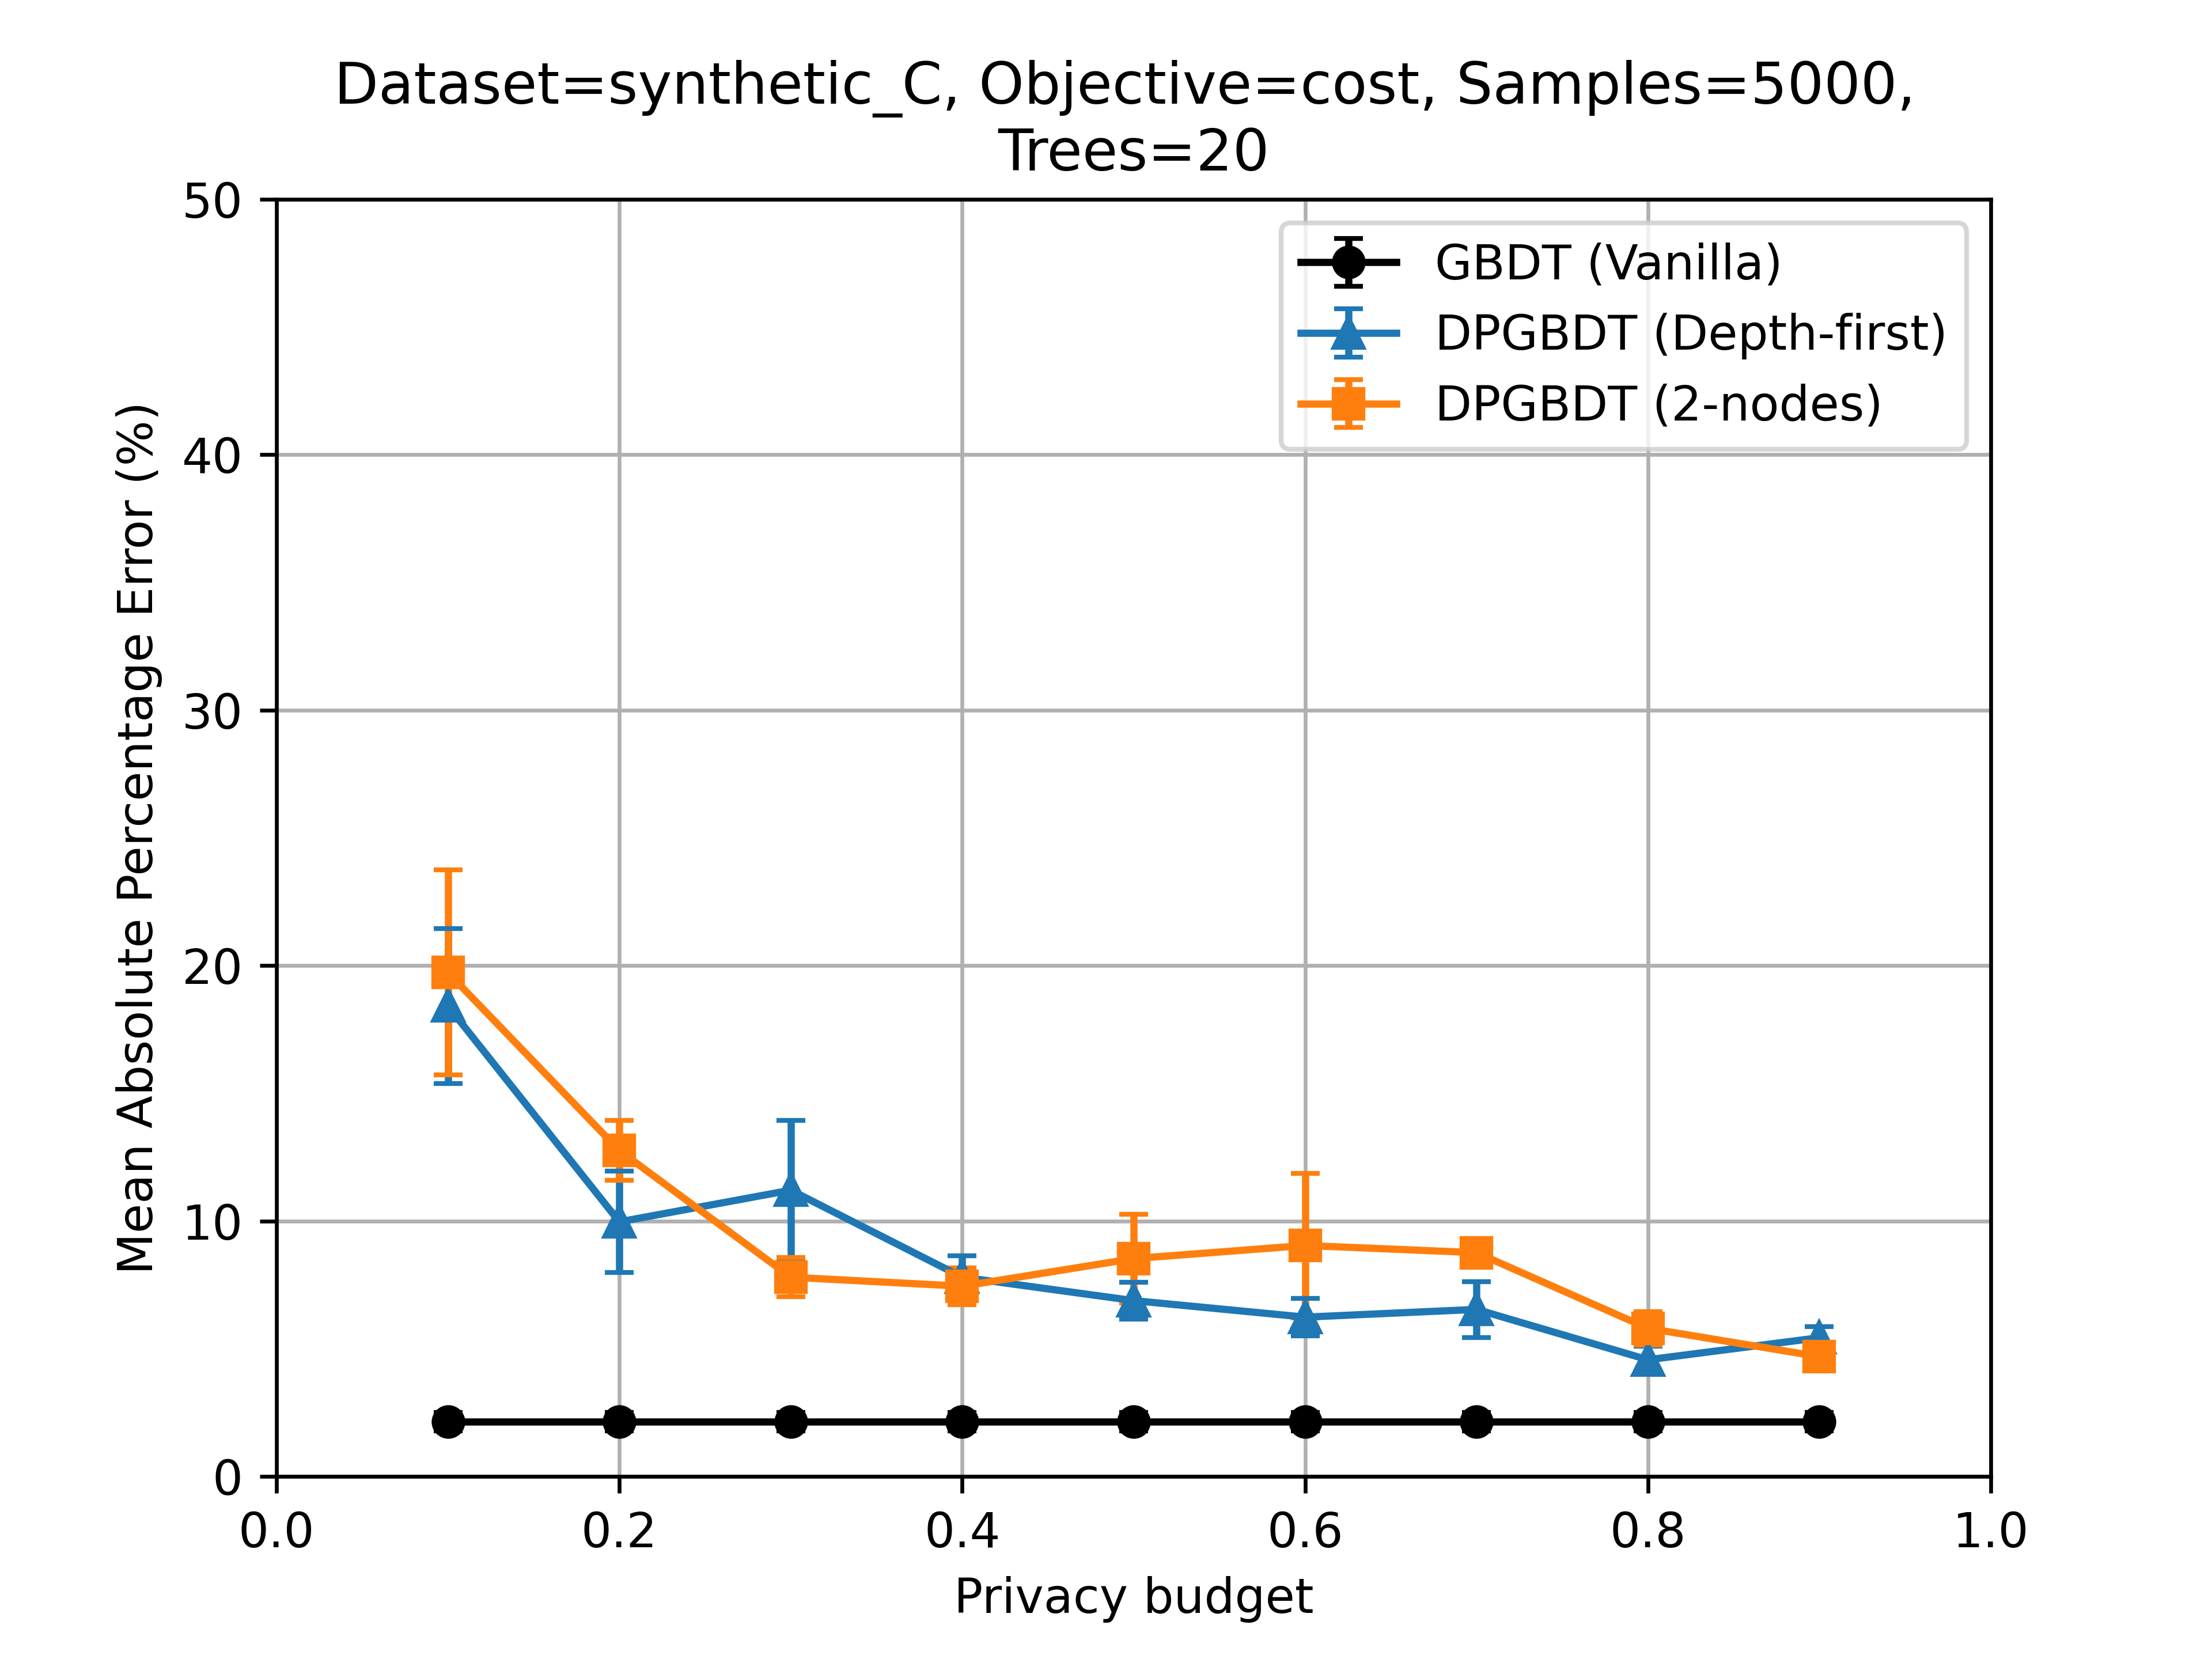
\includegraphics[width=.5\linewidth]{images/evaluation/synthetic_C_cost_5000.png}\hfill
  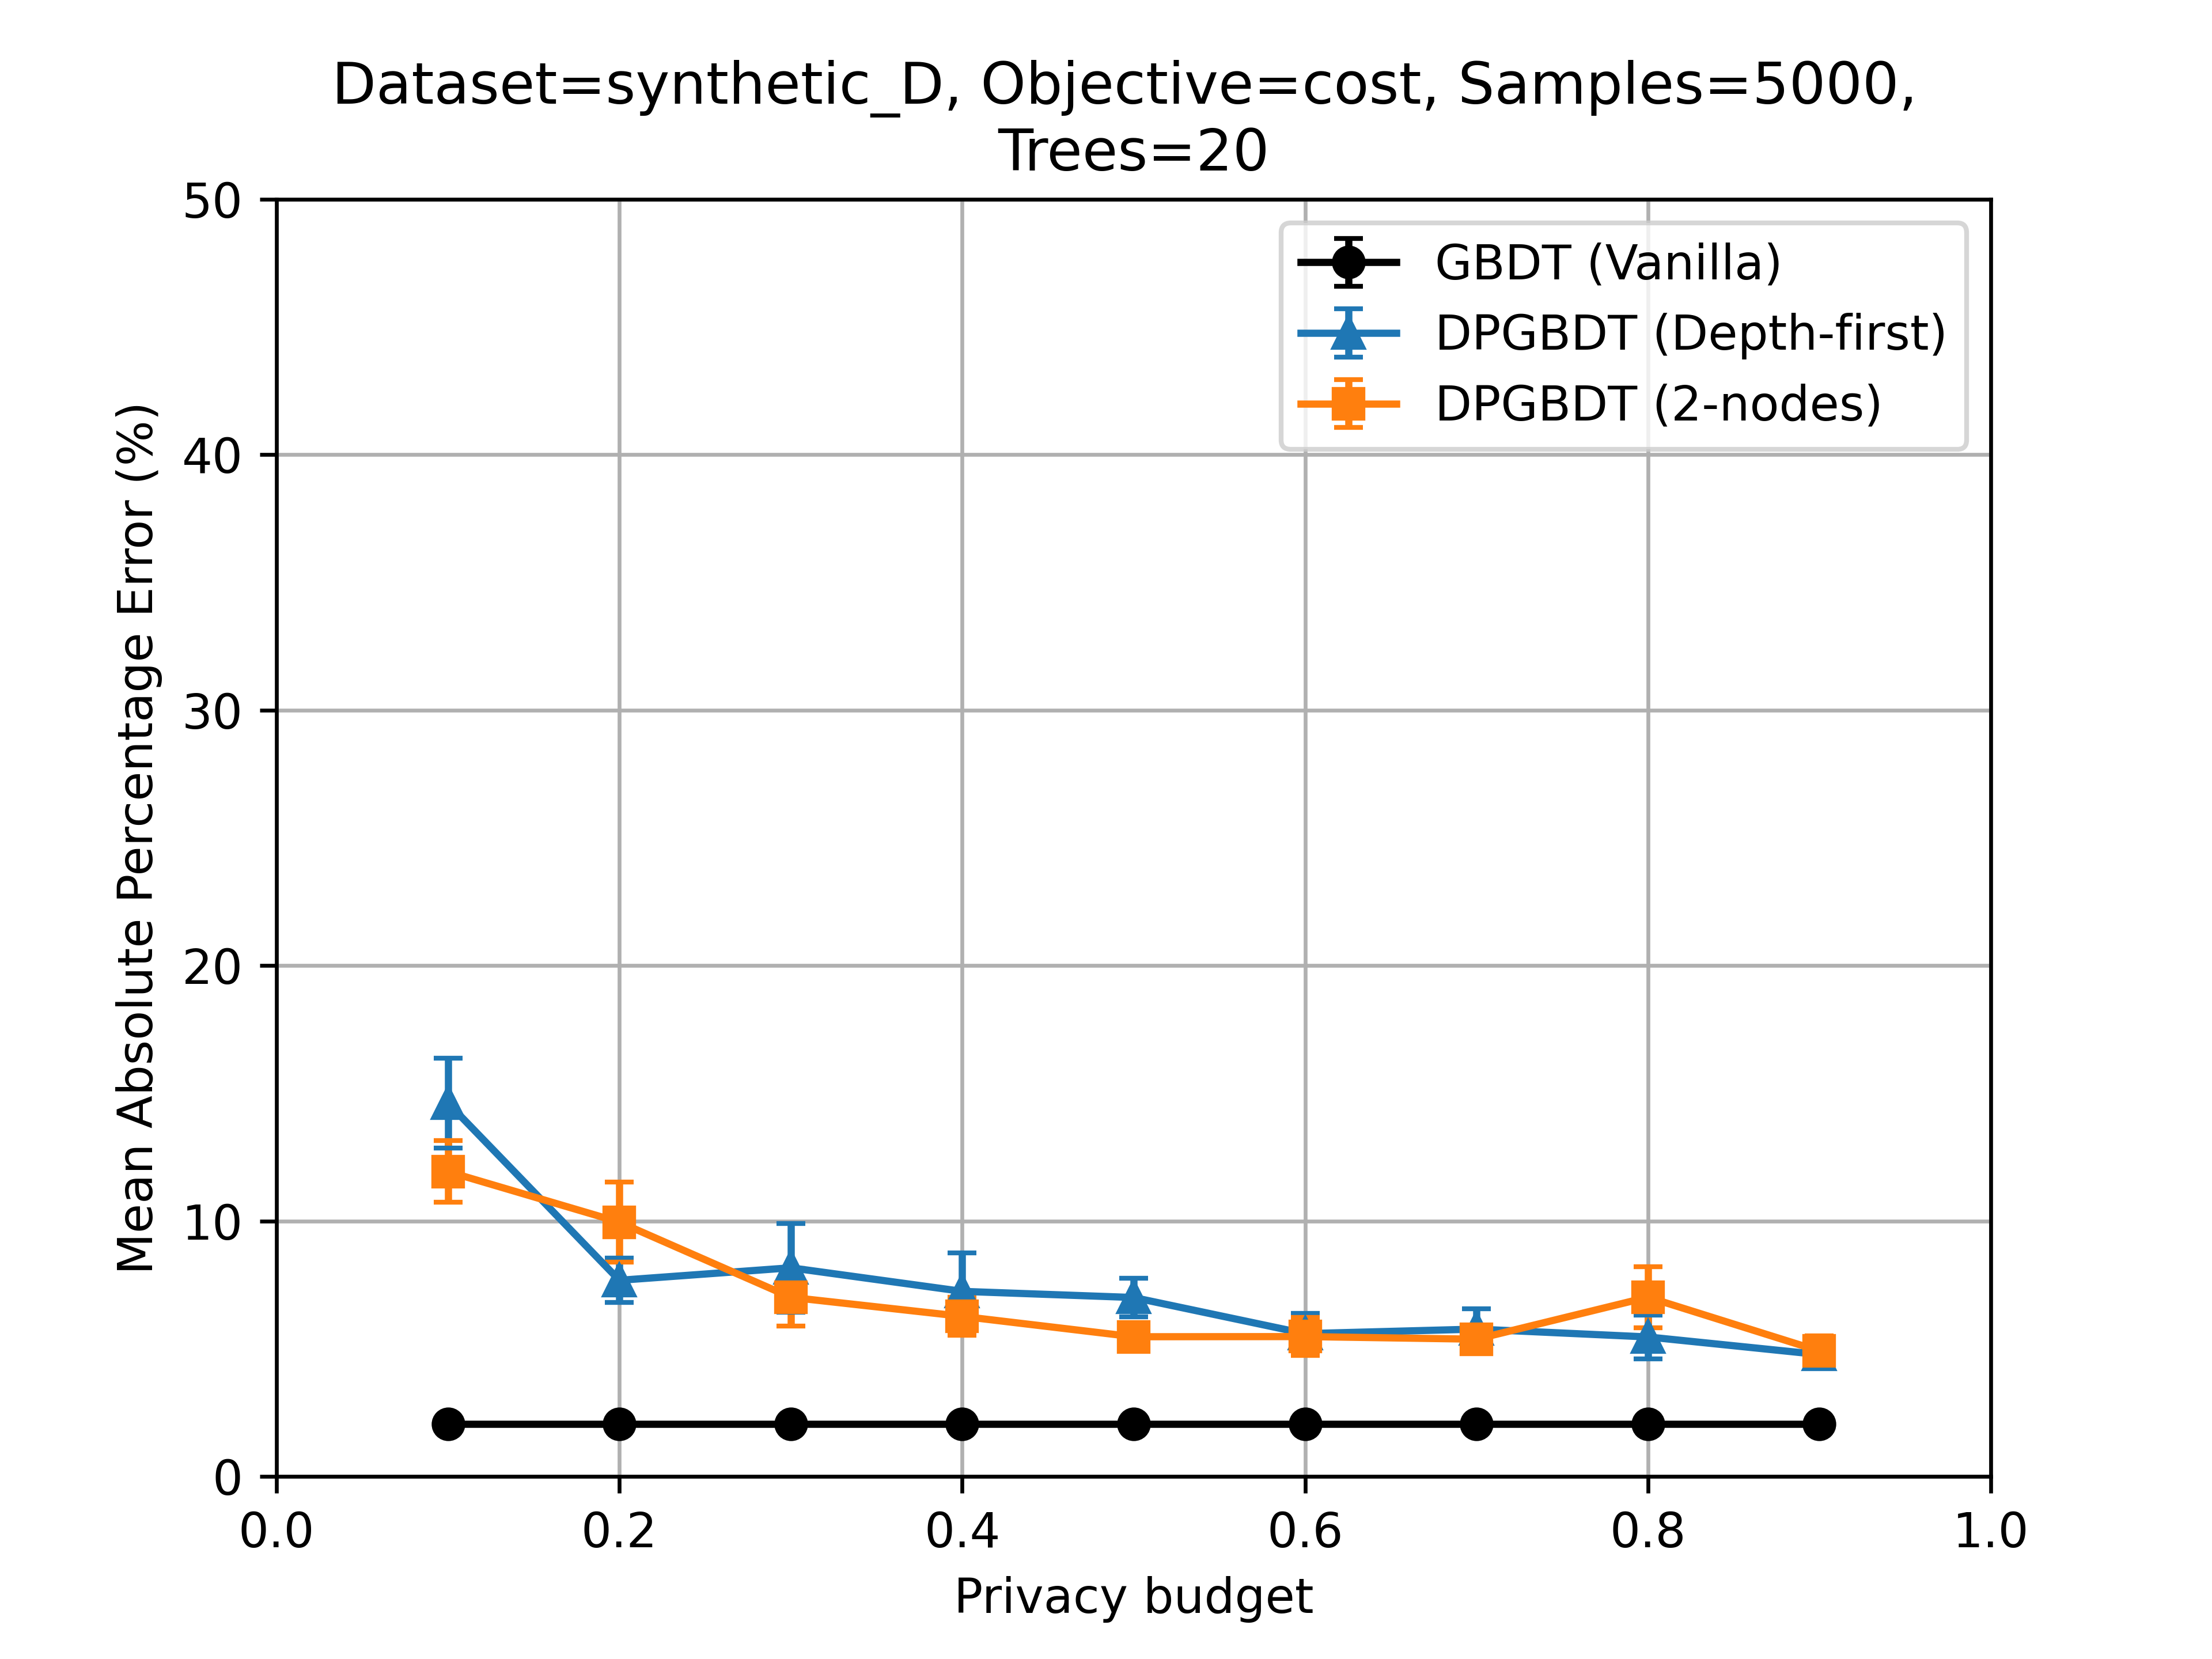
\includegraphics[width=.5\linewidth]{images/evaluation/synthetic_D_cost_5000.png}
  \caption{Synthetic datasets C and D}
  \end{subfigure}
  \caption{\label{fig:results_synthetic_cost}Mean Absolute Percentage Error for the \textit{cost} target on the synthetic datasets.}
\end{figure}

\chapter{Security Analysis}\label{chap:security_analysis}

\section{Attack landscape}

In this section, we give an overview of the various attacks that we consider for our model.

\subsection{Enclave attacks}

Most SGX attacks are side-channel \cite{sgx_survey} attacks, i.e. attacks that are based on information gained from the implementation of the system under attack, rather than weaknesses in the implementation itself. Popular side-channel attacks against SGX are cache-based timing attacks, such as \textit{Flush+Reload} \cite{flush_reload} or \textit{Prime+Probe} \cite{prime_probe}. Both attacks exploit cache behaviour to leak information on victim access to shared memory. In \textit{Flush+Reload}, the attacker flushes a memory line and then measures the time that it takes for the line to be reloaded. If the line was reloaded fast, then the attacker infers that the victim accessed the data located at that line. In \textit{Prime+Probe}, the attacker first primes the cache (i.e. loads it with dummy data) and waits for the victim to access one of the cache lines. Afterwards, the attacker probes the cache and measures its response time. If the access is fast, then the victim did not access this cache line. If it is slow, it did access it. Figure ~\ref{fig:cache} shows how processors fetch data from the cache / memory, and how it relates to access time.

To defend against such attacks, the enclave's authors must make sure that their design is side-channel resilient. This can be achieved by making sure that the code is designed in a cache leakage-free manner, making the execution flow and memory access patterns independent of the data accessed. For other kinds of attacks, \cite{sgx_survey} suggests that authors can act on multiple fronts: microcode patches, system/application design and compiler/SDK. While this is an active and interesting research area, it is mostly independent of the focus of this thesis, and thus we will not explore these attacks further.

\begin{figure}[h!]
	\center
	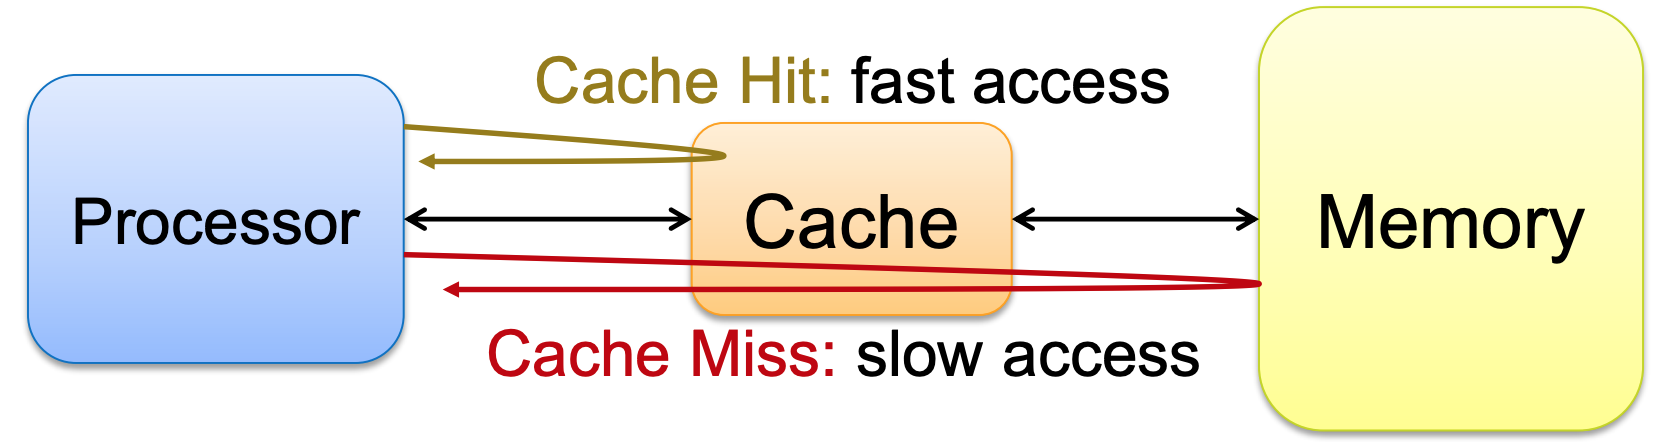
\includegraphics[scale=0.35]{images/introduction/cache}
	\caption{\label{fig:cache} Illustration of a processor fetching data from cache or memory \cite{intel_slides}.}
\end{figure}

\subsection{Security \& privacy attacks}

Since the questionnaires are served to the customers through e.g. a web application, we must consider security attacks targeted at such applications. A malicious customer could try to influence the model accuracy by tempering with the learning set. This could be done by e.g. flooding the web application with bogus questionnaire's answers. In this thesis we will assume that customers are trustworthy, and we will instead focus on privacy attacks, in particular those that target machine learning models.

If a machine learning model was trained using personal data, such as people's health records or identity information, then a privacy attack would aim at extracting these information to benefit the attacking party. For the scope of this thesis, we consider the insurance company to be the adversary, since they own the machine learning model. While they cannot access its content (as it is enclave-protected), it can design privacy attacks in order to gain information about the training set used by the model (i.e. the questionnaires submitted by the customers). Since it is assumed that the model is trained and run within a trusted environment, we will focus our threat model on black-box attacks (i.e. the attacker only has access to the model's API, can submit input vectors and retrieve their corresponding predictions), as shown in Figure ~\ref{fig:threat_model} (adapted from \cite{ml_survey}).

\begin{figure}[h!]
	\center
	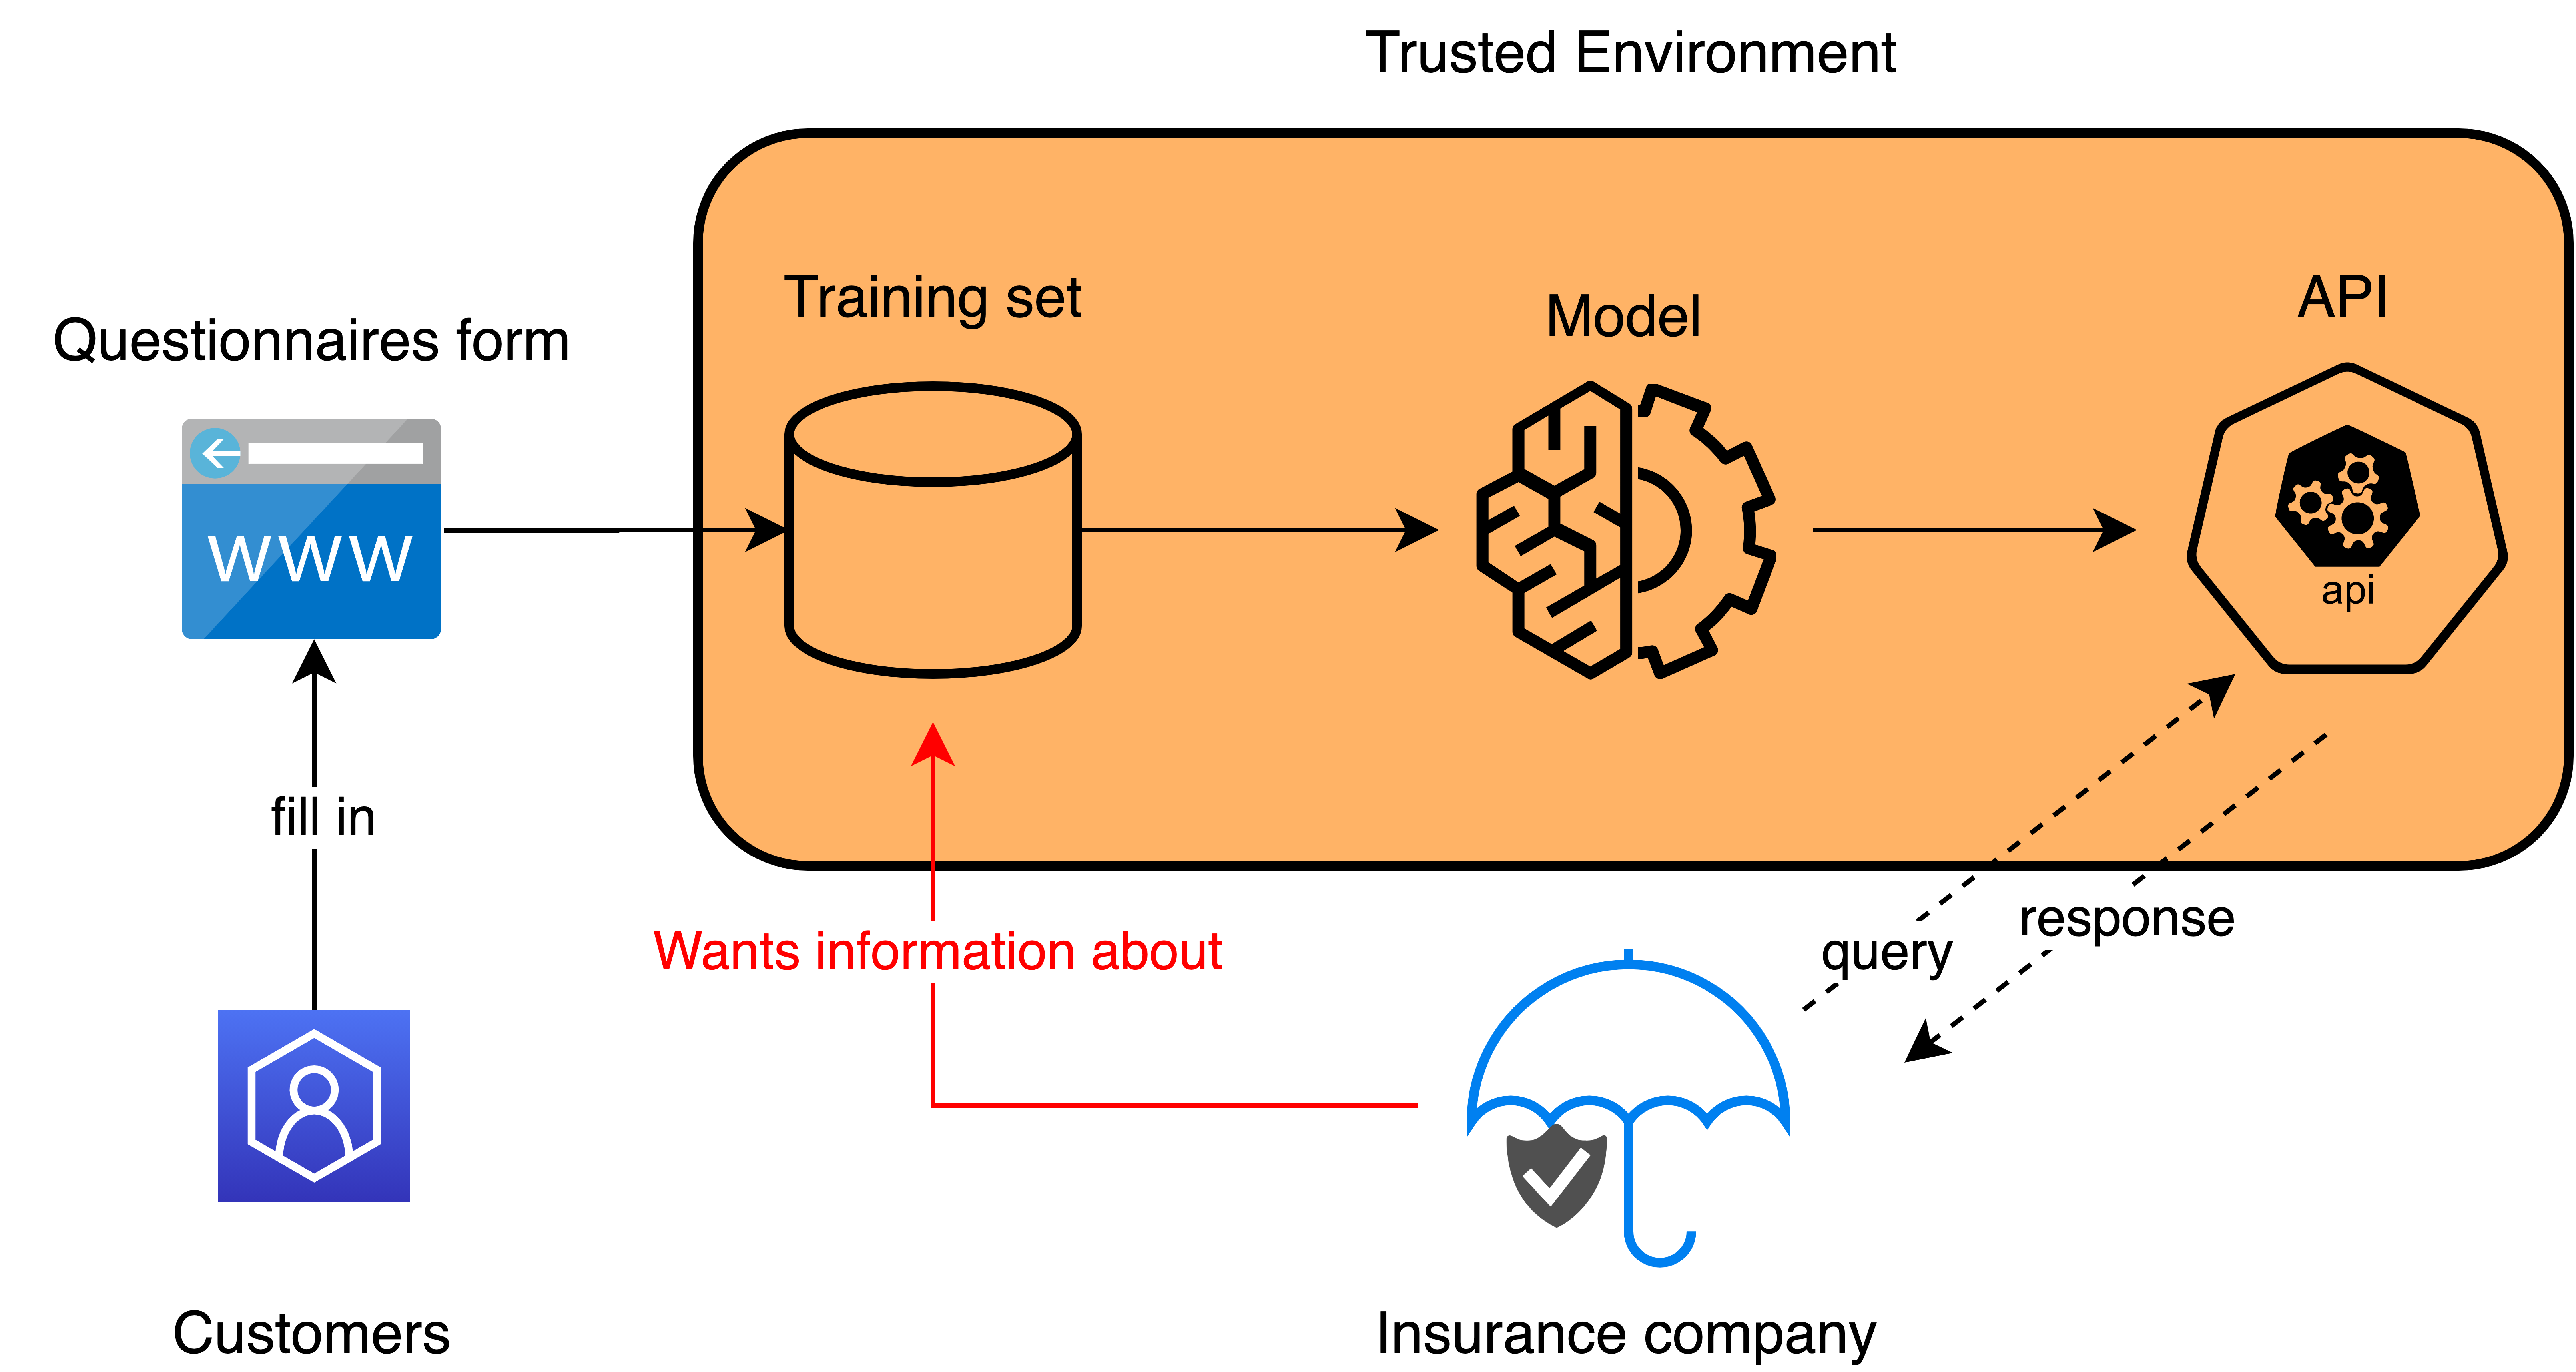
\includegraphics[scale=0.76]{images/introduction/threat_model}
	\caption{\label{fig:threat_model} Threat model}
\end{figure}

In such a model, the insurance company is interested in gaining meaningful information about the training instances that were used by the model. Several attacks can be constructed \cite{ml_survey}:

\begin{itemize}
	\item \textbf{Membership inference attack}: these attacks aim at determining whether or not an input vector $\mathbf{x}$ was used as part of the training set. First introduced by Shokri et al. (2017) \cite{shokri}, it is one of the most popular attacks. This attack assumes a black-box scenario where the attacker only has access to the prediction vectors.
	\item \textbf{Model inversion attack}: given a prediction vector $\mathbf{\hat{y}}$ and partial knowledge of some features of the initial sample $\mathbf{x}$, this attack aims at recovering information about one or all missing features. This is not to be confused with \textit{attribute inference attacks}, which try to infer sensitive feature's values of a targeted instance by leveraging publicly available data.
	\item \textbf{Property inference attack}: these attacks aim at extracting properties over the training set that were not explicitly encoded as features during the learning task. For instance, our synthetic data generation process (described in details in Chapter ~\ref{chap:synthetic_data}) does not encode the number of employees of a company in the dataset. Trying to determine such property from the model would fall under this category of attacks.
	\item \textbf{Model extraction attack}: these attacks do not aim at recovering information about the training dataset, but information about the inner working of the learning model, in order to reconstruct a substitute model that behaves similarly.
\end{itemize}

Many of the above attacks are conducted through \textit{shadow models training}, which is illustrated in Figure ~\ref{fig:shadow}. In shadow training, the attacker trains various models (the so-called shadow models) on shadow datasets, i.e. datasets that follow a similar distribution as the target dataset. Once the shadow models are trained, the attacker constructs an attack dataset, where each instance typically represents the probability vector outputted by the shadow models. The attacker can then train an attack model, which takes as input a prediction vector and outputs membership / property information.

\begin{figure}[h!]
	\center
	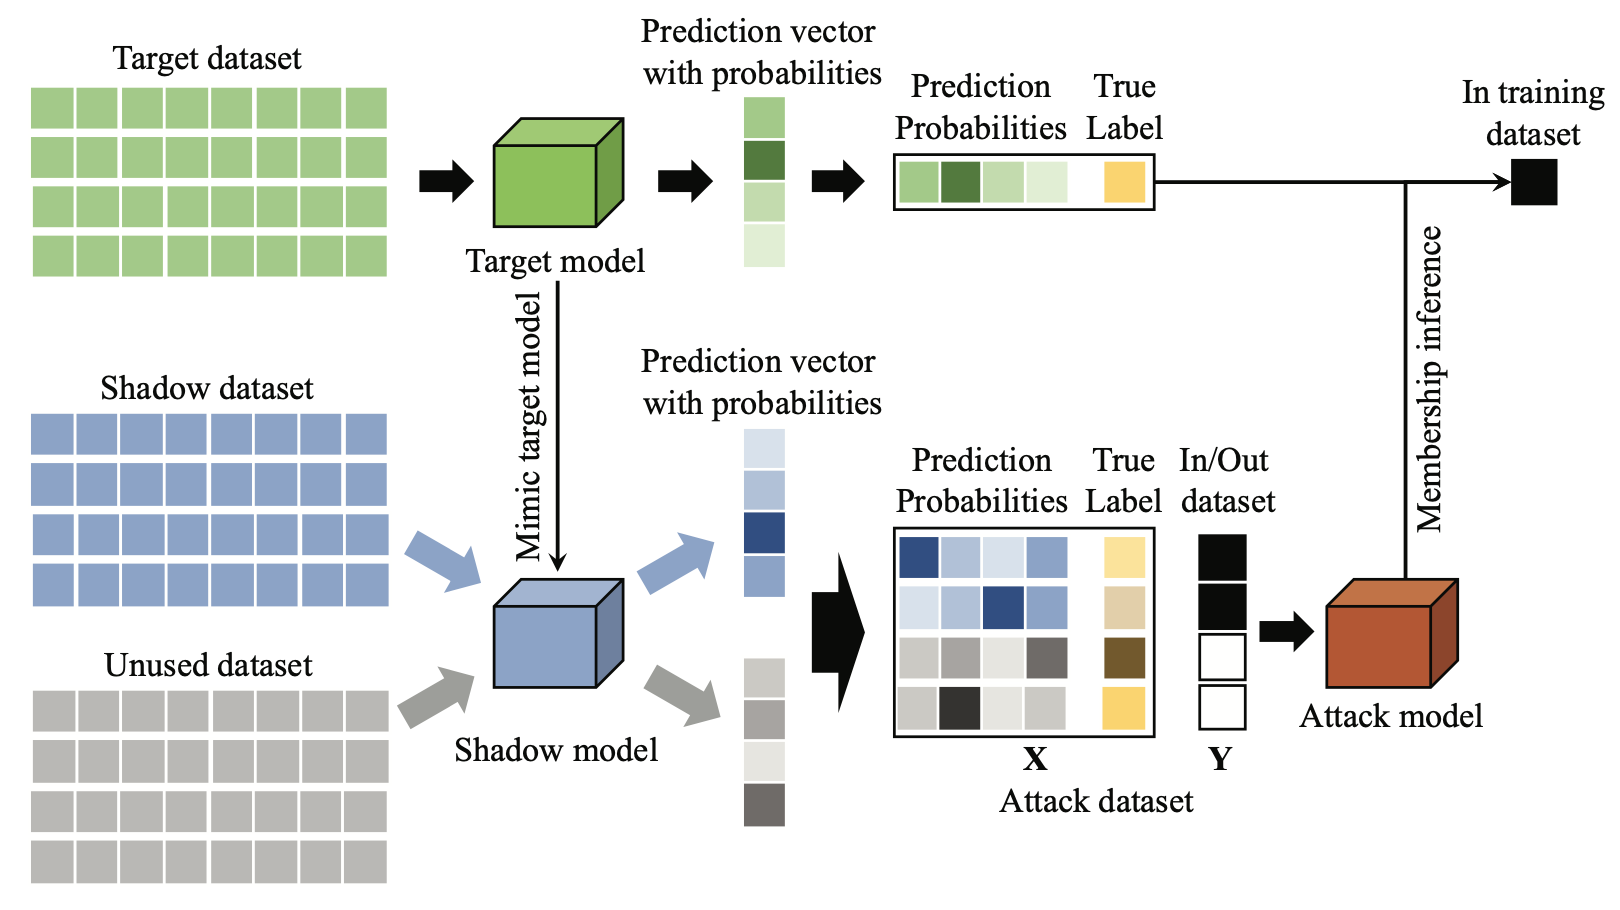
\includegraphics[scale=0.52]{images/introduction/mia}
	\caption{\label{fig:shadow} Shadow training architecture for a membership inference attack. \cite{chen}}
\end{figure}

\section{Attacks on DP-GBDT}

While there are many Python libraries readily available to conduct privacy attacks on machine learning models, such as the \textit{adversarial-robustness-toolbox} Python library\footnote{\href{https://github.com/Trusted-AI/adversarial-robustness-toolbox}{https://github.com/Trusted-AI/adversarial-robustness-toolbox}}, to the best of our knowledge there is no work in the literature that considers privacy attacks on regression models such as our ensemble of gradient boosted decision trees. We therefore tried to convert our synthetic datasets to a classification task, and to tweak our model to support multi-class classification. We evaluate several classical attacks, in particular the gap attack, introduced by Shokri et al. (2017) \cite{shokri}, for different train-test split ratios. Unfortunately, our tests indicate that the current attacks do not adapt well to regression models. In particular, we were unable to detect an explainable correlation between the privacy budget and the accuracy of the membership inference attack. For reference, our results are shown in Figure ~\ref{fig:attack_cost} and summarised in Table ~\ref{table:attack_cost} (for a fixed $\epsilon=0.1$). 

While for low $\epsilon$ values, our model is effectively reducing the success rate of membership inference attacks to $60\%$ or below, the literature (\cite{chen}, \cite{label_only}) shows that we should see such values starting from a higher $\epsilon$ value. Figure ~\ref{fig:attack_cost_50} shows the same attack on a 50-50\% train-test split. From the Figure, what happens is unclear: the model seems not to be leaking any data. However this should be interpreted with a grain of salt, as this could be the result of a lack of better attacks for GBDT models. Indeed, most of current work that evaluates the impact of differential privacy on membership inference attacks targets neural networks and deep learning models only (such as the work in \cite{chen} and \cite{dp_mia}). The reader can refer to Figure 4 in \cite{ref_attack} to get an idea of the influence of differential privacy against membership inference attacks for neural networks.

During this thesis, we have also tried to evaluate the model against other inference attacks, such as attribute inference attacks. Different settings were tested, such as growing very deep decision trees to overfit on the training data. This was done using both the \textit{adversarial-robustness-toolbox} as well as other work found on popular open-source website GitHub. Results were hovering in the 50\% attack accuracy zone, consistently across the different tools, confirming that our model could not be evaluated as-is. This shows that developing privacy attacks on regression ensemble models will be an important step in evaluating them, and we encourage future work in that direction.
\chapter{Related Work}\label{chap:related_work}

In this chapter, we give a brief overview of other privacy preserving work, that use different mechanisms than differential privacy. In particular, we focus on membership privacy.

Nasr et al. (2018) \cite{mia_reg} opt to turn the problem into a \textit{min-max privacy game}, and design a training algorithm that both minimises the prediction loss of the model as well as the maximum gain of the best membership inference attack. By considering the strongest membership inference attack available to an attacker, the defender can ensure that his model will provide the best protection. Their method is designed to work on classification models. They showed that on popular classification dataset Purchase-100, their method only decreased baseline accuracy by 3.6\%, while reducing the membership attack success rate from 67.6\% to 51.6\%.

In \cite{mia_memguard}, Jia et al. (2019) introduced MemGuard. MemGuard offers defences against membership privacy attacks while providing utility-loss guarantees. As opposed to tampering with the training process of the algorithm such as in differential privacy, the authors propose to carefully add noise to the vector of confidence score. This vector is equivalent to the prediction vector with probabilities that is depicted in Figure ~\ref{fig:shadow}. The amount of noise that is added to the prediction vector is not enough to change the predicted label itself, but is enough to trick the adversary's attacking model. 

In their design of a membership inference attack, Shokri et al. (2017) \cite{shokri} also give pointers to mitigation strategies:
\begin{enumerate}
	\item \textbf{Restrict the prediction vector to the top $k$ classes only}: the more classes there are in a dataset, the more information the model leaks. If there are many classes that are present in small quantities only, restricting the model to the top $k$ classes will still result in useful outputs. Having a small $k$ will reduce the attack success.
	\item \textbf{Coarsen precision of the prediction vector}: this is similar to \cite{mia_memguard}, but instead of adding noise to the prediction vector, its probabilities are rounded to $d$ digits. The smaller $d$ is, the less information the model leaks.
	\item \textbf{Use regularization}: since models that overfit too much the data will tend to be more vulnerable to membership inference attacks, regularisation techniques such as the $L_2$-norm standard regularisation can be used to counter overfitting.
\end{enumerate}

As shown in above research, differential privacy is not the one solution to many problems, but rather it is a potential solution to some specific problems, and sometimes differential privacy is not the way to go. Membership privacy (or more generally privacy preserving machine learning) is an active area of research, and there's still room for improvement and for finding a one-fit-all solution. 
\chapter{Conclusion}


\appendix

\chapter{Dummy Appendix}

You can defer lengthy calculations that would otherwise only interrupt
the flow of your thesis to an appendix.




\backmatter

\bibliographystyle{plainurl}
\bibliography{refs}

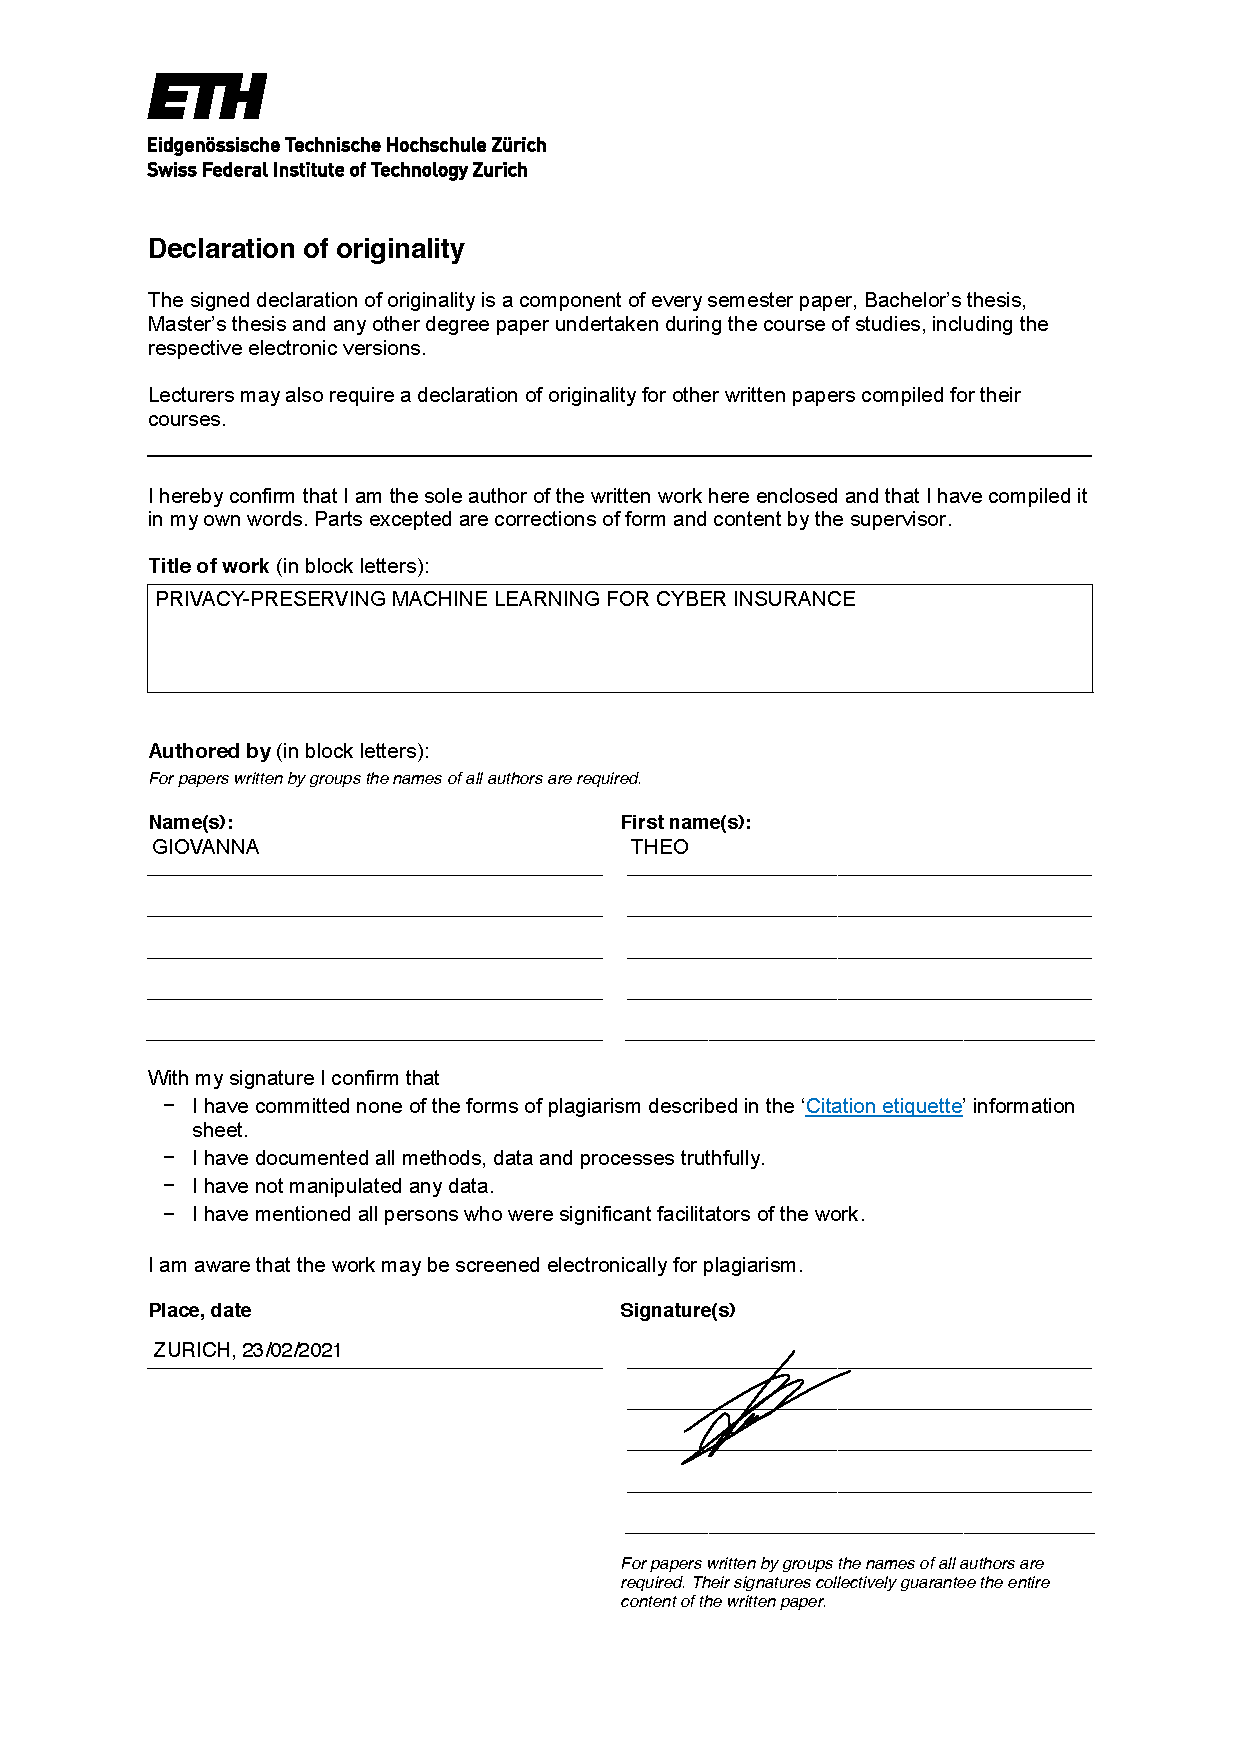
\includepdf[pages={-}]{declaration-originality.pdf}

\end{document}
